%!TEX TS-program = xelatex
%!TEX encoding = UTF-8 Unicode

\documentclass{harvard-thesis}

\usepackage{amsthm}
\usepackage{algorithm2e}
\usepackage[figuresright]{rotating}
\usepackage{multirow}
\usepackage{lscape}
\usepackage{longtable}

% Add macros
\newcommand{\bm}{\vec}
\newcommand{\convolution}{*}
\newcommand{\Reals}{\mathbb{R}}


\def\pythonstyle{}

\ifx \pythonstyle \undefined
\else
\AlgoDontDisplayBlockMarkers \SetAlgoNoEnd \SetAlgoNoLine%
\SetStartEndCondition{ }{}{}%
\SetKwProg{Fn}{def}{\string:}{}%
\SetKw{KwTo}{in}\SetKwFunction{Range}{range}%
\SetKwFor{For}{for}{\string:}{}%
\SetKwIF{If}{ElseIf}{Else}{if}{:}{elif}{else:}{}%
\SetKwFor{While}{while}{:}{fintq}%
\fi

% Macros used in thesis

\newcommand{\E}{\mathbb{E}}
\newcommand{\given}{\, | \,}
\newcommand{\mybox}[4]{\centering
\colorbox{lightgrey}{\parbox{#1\textwidth}{\centering \vskip #3
\begin{minipage}[t]{#2\textwidth} #4 \end{minipage} \vskip #3}}}

\newcommand{\diag}[1]{\mathrm{diag}\left(#1\right)}
\newcommand{\tr}[1]{\mathrm{tr}\left(#1\right)}
\newcommand{\diagvec}[1]{\mathrm{\overrightarrow{diag}}\left(#1\right)}
\newcommand{\unitmat}[0]{\vec{1}\vec{1}^T}
\DeclareMathOperator{\argmax}{arg\,max}
\newcommand{\dd}{\; \mathrm{d}}
\DeclareMathOperator{\Unif}{Unif}
\DeclareMathOperator{\Multinom}{Multinom}
\DeclareMathOperator{\Bernoulli}{Bern}
\DeclareMathOperator{\Poisson}{Poisson}
\DeclareMathOperator{\logit}{logit}
\DeclareMathOperator{\Var}{Var}
\DeclareMathOperator{\Cov}{Cov}
\DeclareMathOperator{\Median}{Med}
\newcommand{\range}[2]{\left\{#1 \ldots #2\right\}}
\newcommand{\fnDef}[3]{#1 \,:\, #2 \rightarrow #3}



\begin{document}

% the front matter
% some details about the thesis
\title{Distributed and Multiphase Inference in Theory and Practice}
\author{Alexander Weaver Blocker}
\advisor{Professor Xiao-Li Meng}

% about the degree
\degree{Doctor of Philosophy}
\field{Statistics}
\degreeyear{2013}
\degreemonth{May}

% about the university
\department{Department of Statistics}
\university{Harvard University}
\universitycity{Cambridge}
\universitystate{Massachusetts}
\maketitle
\copyrightpage
\abstractpage
\tableofcontents
\dedicationpage
\authorlist
\acknowledgments

% include each chapter...
\include{chapters/chapter-nucleosomes}
%!TEX TS-program = xelatex
% !TEX root = ../thesis.tex
% Do not delete; used to set build system

%\begin{savequote}[75mm] 
%Nulla facilisi. In vel sem. Morbi id urna in diam dignissim feugiat. Proin molestie tortor eu velit. Aliquam erat volutpat. Nullam ultrices, diam tempus vulputate egestas, eros pede varius leo.
%\qauthor{Quoteauthor Lastname} 
%\end{savequote}

\chapter{Full-proteome absolute quantitation from label-free LC-MS/MS experiments}
\label{proteomics:ch:proteomics}

\section{Introduction}
\label{proteomics:sec:intro}

Proteins are the leading actors in cellular processes, making them a prime target for biological investigation.
Understanding their absolute concentrations within a population of cells can elucidate the molecular dynamics that regulate their functions \citep{Ishihama:2005ir} and open a broad range of biological processes to deeper investigation.
However, measuring the concentration of many proteins in a single experiment has been difficult until very recent \citep{Ghaemmagham:2003tu}. 
As a result, many investigations have relied upon gene expression as a proxy for the concentration of these proteins; this is, at best, an imperfect substitution.
In recent years a new field of high-throughput proteomics has emerged, in which biologists and biochemists have begun exploring the next level of biological complexity with Fourier transform mass spectrometers  \citep{Scigelova:2006p10560,Scigelova:2011dt}.
This technology has dramatically shifted in our ability to measure the concentration of proteins and other small molecules.
Whereas low-throughput proteomic studies have been able to identify a few important proteins involved in each function, high-throughput mass spectrometry can deliver a fine-grained view of cellular activity at an unprecedented scale and precision.
In principle, this new technology enables the direct estimation of absolute protein concentrations from the relative intensities of protein fragments in a biological sample.

In practice, the measurement process implemented by mass spectrometers introduces complex systematic biases that must be accounted for to obtain valid estimates of absolute protein concentrations.
Proteins are large macromolecules, consisting of intricately-folded sequences of amino acids. 
They are enzymatically digested into fragments, which are amenable to analysis by mass spectrometry \citep{Thakur:2011kz}. 
% Introduce distinction between fragments (unidentified peptides) and peptides (identified up to a modification or charge state).
Protein fragments are generally referred to as {\em peptides}; throughout this paper, fragments with the same sequence but distinct characteristics (e.g., charge states and chemical modifications) are considered {\em distinct} peptides. 
%A typical biological sample contains hundreds of thousands of peptides. 
These peptides are analyzed by two separate mass spectrometers to produce quantitative summaries \citep{Steen:2004tk}.
 However, because of sample complexity and instrument limitations, not all of the peptides can be analyzed in the second-stage of mass spectrometry to have their sequence identified.
The instrument is programmed to select the most abundant peptides in the first stage of mass spectrometry for sequencing, at any given time.
This multi-stage measurement process results in a systematic bias towards observing peptides from the sample's most abundant proteins.
In this paper, we present and evaluate a statistical technique to correct these biases, providing reliable estimates of absolute protein abundances from mass spectrometry experiments.

Figure \ref{proteomics:fig:Mass_Spec_Overview} illustrates the experimental process underlying our data in detail.
%
\begin{figure}[t]
 \centering
% \includegraphics[width=\textwidth]{figures/proteomics/MS_Overview_small}
% \caption{MS proteomics overview. 
% (A) From cells to protein fragments. 
% (B) Fragments are separated in time, charged with ions, then analyzed using two mass spectrometers.
% (C) The HPLC separates the peptide
%mixture as well as determining the relative abundance of the mixture
%at each time point. MS1 determines the intensities of each compontent
%of the mixture at the given timepoint. Finally, the MS2 determines
%the sequence of a subset of peptide states.}
 \includegraphics[width=\textwidth]{figures/proteomics/mass-spec-errors-awb}
 \caption{LC-MS/MS proteomics overview. 
 Clockwise from top left: Cells are lysed to extract proteins, which are broken down into fragments by a protease.
These fragments are then fractionated by charge and separated by hydrophobicity in the liquid chromotography (LC) stage before being sent through tandem mass spectrometry (MS/MS).
This yields the spectrographic intensity (shown by shaded dots) and mass/charge ratio for each fragment retention time.
A subset of these fragments are selected for further processing at each time, allowing for identification.
\label{proteomics:fig:Mass_Spec_Overview}}
\end{figure}
%
Starting from the top left, a culture of approximately $10^{8}$ cells are opened (lysed) to extract their proteins, which are then digested with an enzyme (protease) into fragments (peptides).
These peptides are then separated by their hydrophobicity via high-performance liquid chromatography (HPLC), which allows them to enter the next stage gradually.
As these peptides exit the HPLC, they are given an electrical charge by electrospray ionization.
All of these steps simply transform the long, complex mass of proteins from our cell culture into a well-separated set of simpler molecules that the mass spectrometers can process.

Fragments that are ionized within the same short time window are analyzed simultaneously by the first of two mass spectrometers (MS1).
At this stage, fragments with the same sequences of amino acids are present in a number of different states as a result of ion charges, \emph{in vivo} post-translational modifications and \emph{in vitro} chemical modifications from the sample preparation \citep{Michalski:2011gm}.
This step results in measurements $\xi(t, r)$ each of which quantifies the intensity\footnote{This intensity corresponds to the magnitude of a Fourier coefficient associated with peptides of mass-to-charge ratio $r$. Modern mass spectrometers generally measure the amplitudes at which ionized protein fragments oscillate along an electrode over time. The Fourier transformation $\xi(f)$ of the amplitude time series from a mixture of ionized fragments provides the power associated with each frequency $f$. Each frequency $f$ is associated with fragments of a particular mass-to-charge ratio $r$ according to $f=C/r$, where $C$ encodes instrument geometry and settings, yielding $\xi(t, r(f)) = \xi(t, r)$ \citep{Scigelova:2006p10560}.
% m/z in dalton/charge
% (obs m - true m)/(tr m)*1M in ppm
% f = k*B/(2*\pi*m/z) with f=axial freq, B=force of EM field, and m/z as above -- in orbitrap} %%% brief explanation of intensity %%%
}
%
corresponding to ionized fragments with mass-to-charge ratio $r$, analyzed within a time window indexed by $t$.
These intensities are proxies for relative abundance of fragment in the mass spectrometer within each time window.
%
The rightmost sections of Figure \ref{proteomics:fig:Mass_Spec_Overview} illustrates the output of this process, with each fraction yielding a set of intensities $\xi(t, r)$ for each retention time and mass-to-charge ratio.
The lower right panel of this figure shows one slice through this dataset corresponding to a particular time $t$.

A subset of the fragments analyzed by the first mass spectrometers is selected, based on their intensities, to be broken down into yet simpler molecules by collision with a gas (CID).
The products of these collisions are then analyzed by a second mass spectrometer (MS2).
This step results in an additional set of intensity measurements for these components, each of which has a distinct mass-to-charge ratio and is associated with its original fragment's mass-to-charge ratio by the instrument.
The final (bottom left) panel of Figure \ref{proteomics:fig:Mass_Spec_Overview} shows the intensity spectrum obtained by MS2 for the components of the fragments with mass-to-charge ratio $r$ selected from MS1.
The amino acid sequence of these fragments can be reliably determined by analyzing differences in the mass-to-charge ratio between adjacent peaks in the MS2 spectrum.
%Peptides with exactly the same mass-to-charge ratio and sequence bits cannot be distinguished, but this occurs quite rarely give the accuracy of the instrument (1-2 parts-per-million) and the combinatorial explosion in the number of peptides---possible fragments times possible ion charge states times possible post-translational and chemical modifications.

% two stat problems: identification/matching, absolute abundance estimation.

The statistical problem of interest is to estimate the absolute concentrations of proteins in our sample from the observed peptide-level intensities $\{\xi(t, r):t\in T,r\in R\}$.
However, to tackle this problem, we must first associate these raw intensities with peptides and condense them into a more manageable set of summaries.
This preprocessing falls under the heading of identification, a well-studied problem in MS/MS proteomics.
%
In the identification task, the intensity and mass-to-charge data from MS2 are used to detect which peptides are present in the sample, in terms of their most likely sequence, charge, and possible chemical and post-translational modifications.
In a typical run, hundreds of thousands of unique peptides are simultaneously detected.
The observed spectrum of each detected peptide is then compared to the theoretical spectra of the all peptides that would be generated by digesting the proteins in the sample with a specific enzyme.
For example, the enzyme trypsin digests the amino acids arginine (R) and lysine (K), so each protein is expected to be fragmented into peptides by removing all arginines and lysines from its amino acid sequence.
Currently, several well-established methods for peptide/protein identification exist in the literature \citep{Cox:2008uu,Perkins:1999ed,Eng:1994fj}; we generally use the MaxQuant software of \citet{Cox:2008uu}.

Identification yields a set of integrated log-intensities $y_{ikl}^{obs}$, each of which is associated with a protein $i$, peptide $k$, and state $l$, where by state we refer to modifications, charges, etc.
These are known to be approximately linearly related of log of the number of molecules of that peptide present in the mass spectrometer, making them an excellent basis for absolute quantitation \citep{Old:2005jf,Scigelova:2011dt}.
Formally, each $y_{ikl}$ comes from two operations: a mapping between identified fragment and a given set of values for $(t, r) \in \Delta_{ikl}$, and the integration of $\xi(t,r)$ over these values.
%
The mapping serves to associate each observed $\xi(t, r)$ with a given peptide state $ikl$.
The raw intensities $\xi(t, r)$ are then integrated over a small window in both retention time and mass-to-charge ratio.
The former accounts for the fact that any given peptide $ikl$ is typically observed across adjacent time windows, while the latter accounts for minor variation in $r$ for each fragment originating from the presence of multiple isotopes and other factors.
Thus, all of our inferences are based on
%
\begin{equation}
y_{ikl}^{obs} = \log_{10}\left( \int \! \int_{(t, r) \in \Delta_{ikl}} \xi(t, r) \dd r \dd t \right) .
\end{equation}

With these quantities in-hand, we can refine the statement of our statistical problem: using the collection of integrated log-intensities $y_{ikl}^{obs}$ and known properties of the observed proteins, estimate the log-absolute concentrations of proteins in our sample $\zeta_i$.
We present a probabilistic model for these data in Section \ref{proteomics:sec:model}, with particular details of the core estimand $\zeta_i$ provided in Section \ref{proteomics:sec:estimand}.



\subsection{Related work}

There are two threads of literature on protein quantitation: relative and absolute quantitation. 
In relative quantitation, the estimand of interest is the ratio of a given protein's concentrations in two distinct samples  (generally different experimental conditions).
In contrast, absolute quantitation requires the ability to estimate the concentrations of all proteins in a single sample, relative to one another---these quantities together with the total amount of protein measured in a sample lead to the estimands of interest in our work, $\{\zeta_i:i\in I\}$, as we discuss in Section \ref{proteomics:sec:estimand}.


While there has been much work on the problem of peptide identification \citep[e.g.,][]{Cox:2008uu,Perkins:1999ed,Eng:1994fj}, less progress has been made on the quantitation problem \citep{Makawita:2010eg}.
Despite the relatively strong correlation between the amount of each protein in a sample, the observed intensities, and the number of its peptides identified by the mass spectrometer \citep{Old:2005jf}, heterogeneity in this relationship between labs, samples, and even peptides from a common protein has hampered the development of robust quantitation methods \citep{Tabb:2010bc,Bell:2009il}.
To control for these sources of variation, the most mature methods for relative quantitation rely on physically labeling each sample being compared, analyzing them simultaneously, and estimating the relative abundance protein-by-protein based on summaries of peptide intensity ratios \citep{Ong:2002tf}.
%
The most common experimental methods for estimating absolute abundance are quite intricate.
For each protein of interest, the experimenter must synthesize a set of synthetic, standard peptides.
They then compare the observed intensities of peptides from the sample to the intensities of the corresponding standard peptides, which are introduced at known concentrations \citep{Gerber:2003kq}.
These approaches have limited throughput, are experimentally complex, and are limited to quantitation of a preselected set of proteins.

Motivated by the limitations of experimental quantitation methodologies, there has been a growing interest in computational methods that can be applied to a variety of samples and settings.
The simplest of these are based on spectral counting, either in the form of ratio-based estimates for relative quantitation \citep{Liu:2004hv}, or using rescaled counts for absolute quantitation \citep{Ishihama:2005ir}.
More recently, a semi-supervised absolute quantitation method called APEX has been developed, which uses a large training dataset to learn how differences in physiochemical properties affect the probability of peptide identification, independent of abundance \citep{Lu:2006p10143}.
It then uses these estimated probabilities of identification to construct a weighted estimator of protein abundance.
%
Another class of methods uses peptide intensities, which have a wider dynamic range than spectral counts, for quantitation, the most common of which are based on simple summaries of observed intensities, such as their median \citep{deGodoy:2008jk, Silva:2005cn}.
Most recently, a few attempts have been made to combine intensity and identification information, for example using principle component analysis to combine these features across samples \citep[e.g.,][]{Dicker:2010ea}.
Finally, the most sophisticated techniques, which motivated our own work, are model-based methods for relative quantitation that account for missing data at the peptide level \citep{Karpievitch:2009wb,Luo:2009ff}.
However, by focusing on peptide-level missingness, these methods fail to account for the true amount of missing data, since each peptide is generally found in a number of different states, due to biological and chemical modifications \citep{Michalski:2011gm}.

%This is due, in part, to the misconception that the measurements produced by the mass spectrometer are extremely accurate and thus there is no need for any statistics after identification. This argument, however, is flawed. It ignores the selection bias implemented at multiple data collection stages within the instrument.
%This bias is especially significant for peptides and proteins present at low concentrations.
%In our work, we proposed a modeling framework that is able to account for and mitigate the selection bias. 
%
%Most of the existing literature is devoted to the relative quantitation task.
%In this case, the consequences of selection bias are arguably mitigated, at least from an empirical perspective.
%Because of this, the most popular methods available for relative quantitation do not involve statistical modeling.
%Rather, they are based on observable summaries produced by the identification procedures, for example spectral counting \citep{Liu:2004hv} and median intensity \citep{deGodoy:2008jk,Silva:2005cn}.
%As we show in Section \ref{proteomics:sec:empirical}, these methods perform poorly when adapted to the task of absolute quantitation as the estimates often span a limited range of absolute concentrations \citep{Schulze:2010fk}.
%
%There are only a handful of model-based methods for either absolute or relative quantitation, and they take very different approaches.
%A semi-supervised approach called APEX uses a training set of proteins to learn the physicochemical properties of peptides that influence their likelihood of detection, which is then used to compute the absolute abundance based on the number of peptide identifications weighted for their "detectability" \citep{Lu:2006p10143}.  More recently, a similar approach has been suggested that relies on principal component analysis and a kernel ... \citep{Dicker:2010ea}.
% An alternative approach relies on a different experimental protocol and technology, but ... \citep{Luo:2009ff}.
% Perhaps closest to our approach, \citet{Karpievitch:2009wb} develop a model that posits a non-ignorable observation model.
%The observation model is specified on peptide-level intensities.
%We show that there is little information at the peptide-level about the censoring process that can be leveraged to correct for the selection bias.
%Instead, our model specifies the observation model in terms of the intensities of peptides in different charge and chemical modification states, a level of measurement where  information about the selection bias can be found in the shared number of states among peptides present a high and low concentrations in the sample.
%Generally, existing methods for absolute quantitation also suffer from limited range of the estimated concentrations \citep{Schulze:2010fk}.

\subsection{Contributions of this article}

In this paper, we introduce a statistical model that combines a hierarchical intensity model with an observation model for intensity-based censoring, in Section \ref{proteomics:sec:model}.
This model accounts for key aspects of the biology and of the data acquisition process, including the fact that peptides are observed in multiple charge and modification states, and that there are at least two missing data mechanisms that compound throughout any LC-MS/MS instrument.

Our approach is novel in a number of ways: 
 (1) the focus is on absolute, rather than on relative quantitation;
 (2) while most existing approaches to quantitation involve simple summary statistics after identification, we posit and estimate a realistic censoring mechanisms that results in non-ignorable missing data;
 (3) the model explains the variability in the  intensities of peptides observed in multiple charge and modification states, rather than the aggregated intensities for individual peptides.  
%
We find that accounting for non-ignorable missing data helps reduce the selection bias induced by the measurement process.
In addition, modeling intensity-based censoring at the level of peptide states helps transfer information from abundant to rare proteins, since the number of states we expect to see any give peptide is independent of abundance.
These aspects of the model allows robust, accurate estimation of absolute protein abundances in complex samples with concentrations spanning many orders of magnitude.

We provide efficient inference for this model, in Section \ref{proteomics:sec:estimation}, by leveraging a combination of Halley's method, adaptive Gauss-Hermite quadrature, and explicit envelopes for sampling the number of censored peptide states and censored intensities.
In Section \ref{proteomics:sec:simulations}, we explore the frequentist coverage of interval estimates, and we compare the performance of the proposed method with existing methods for estimating absolute protein concentrations, as we systematically vary the abundance and the length of the target proteins.
In Section \ref{proteomics:sec:empirical}, we explore the extent to which key assumptions of our model hold in practice, and we analyze estimates based on three biological samples, processed with different LC-MS/MS settings, in which a set of proteins with known concentration was introduced for validation purposes.


 %%% %%% %%%
 %%% %%% %%%


\section{Model}
\label{proteomics:sec:model}

We develop a probabilistic model that describes the complex relationship between the protein properties of interest and the output of an LC-MS/MS experiment.
This includes both the non-ignorable missing data mechanism induced these experimental techniques and the hierarchical structure of our observations.
The observed data consists of two components: the observed state-level intensities $y_{ikl}^{obs}$, indexed by protein $i$, peptide $k$, and charge state $l$, and the observed counts of observed states by peptides $s_{ik}^{obs}$.
We also know the number of possible peptides per protein $m_i$, which is independent of the sample in theory, but which requires careful preprocessing.

We are interested in inferring the abundance of each protein $i$ within the given sample.
This abundance is a monotone function of the parameter $\mu_i$ in the following model:
%
\begin{align}
%1 / \tau_i^2 &\sim \text{Gamma}(\alpha_\tau, \beta_\tau) \\
%1 / \sigma_i^2 &\sim \text{Gamma}(\alpha_\sigma, \beta_\sigma) \\
 \gamma_{ik}\mid\mu_{i}, \tau_{i}^2  &\sim \hbox{Normal}(\mu_{i},\tau_{i}^{2}), \, i=1,\ldots,n, \, k=1,\ldots,m_i \\
 s_{ik} \mid \lambda, r  &\sim 1+\hbox{ Negative-Binomial }(1-\lambda,r), \, k=1,\ldots,m_i \\
 y_{ikl} \vert \gamma_{ik}, \sigma_{i}^2   &\sim \hbox{Normal}(\gamma_{ik},\sigma_{i}^{2}), \, l=1,\ldots,s_{ik}\\
 R_{ikl} \vert \pi^{rnd}, s_{ik} &\sim \hbox{Bernoulli}(1 - \pi^{rnd}), \, l=1,\ldots,s_{ik} \\
 I_{ikl} \vert y_{ikl}, \bm \eta, s_{ik}, R_{ikl}=1 &\sim \hbox{Bernoulli}(1 - g(y_{ikl}; \bm \eta)), \, l=1,\ldots,s_{ik} \\
 O_{ikl} &= R_{ikl} \cdot I_{ikl} \\
 Y_{obs} &= \{y_{ikl} : O_{ikl} = 1\} \\
 Y_{mis} &= \{y_{ikl} : O_{ikl} = 0\}
\end{align}
%
This model can be considered in two pieces: the distribution of the complete data $Y_{com} = (Y_{obs}, Y_{mis})$ given the parameters, and the distribution of the observed data given the complete data and parameters.
Starting with the complete data for protein $i$, this model specifies that each peptide gets a mean intensity $\gamma_{ik}$ distributed about the protein-mean $\mu_i$.
Similarly, each state-level intensity $y_{ikl}$ is distributed about the peptide-level intensity.
The variances of these distributions are $\tau^2_i$ and $\sigma^2_i$, which are themselves drawn from inverse-Gamma distributions.
%
\begin{align}
1 / \tau_i^2 &\sim \text{Gamma}(\alpha_\tau, \beta_\tau) \\
1 / \sigma_i^2 &\sim \text{Gamma}(\alpha_\sigma, \beta_\sigma)
\end{align}

This is a straightforward Normal hierarchical model except for one complication.
%
The number of states per peptide $s_{ik}$ is drawn from a shifted negative binomial distribution.
This distribution is fixed across proteins and peptides, reflecting the physical independence between the number of possible charge states and a protein's abundance.
This invariance plays a crucial role in our inference, as we discuss in Section \ref{proteomics:sec:estimation} and \ref{proteomics:sec:remarks}.
Hence, we have
\begin{align}
\label{proteomics:eq:complete_data_likelihood}
P(Y_{com} | \bm \mu, \bm \sigma^2, \bm \tau^2, r, \lambda) =
\prod_{ik} \Bigg[& \frac{1}{\tau_i} \phi\left( \frac{\gamma_{ik} - \mu_i}{\tau_i} \right)
\begin{pmatrix} s_{ik} + r - 2 \\ s_{ik} - 1 \end{pmatrix} \lambda^{r} (1 - \lambda)^{s_{ik} - 1} \cdot \\
\nonumber
& \prod_{l=1}^{s_{ik}} \left[ \frac{1}{\sigma_i} \phi\left( \frac{y_{ikl} -  \gamma_{ik}}{\sigma_i} \right) \right] \Bigg],
\end{align}
where $\phi(z)$ is defined as $\frac{1}{\sqrt{2 \pi}} \exp\left( -\frac{1}{2} z^2 \right)$.


 %%% %%% %%%

\subsection{Missing data mechanism}
\label{proteomics:sec:mdm}

The missing data mechanism operates at the state level and is characterized via a pair of random variables.
The first variable is $R_{ikl} \sim \text{Bernoulli}(1 - \pi^{rnd})$, the random censoring indicator, which accounts for censoring due to factors other than abundance.
The second is $I_{ikl} \sim \text{Bernoulli}(1 - g(y_{ikl}; \bm \eta))$, the intensity censoring indicator, which accounts for the intensity-dependent component of our missing data mechanism.
Note that we assume $I_{ikl}$ is drawn only if $R_{ikl} = 1$, as shown in Figure \ref{proteomics:fig:Missing_Data_Indicators_Tree}.
%
\begin{figure}[ht!]
\begin{center}
\includegraphics[width=.75\textwidth]{figures/proteomics/fig_tree_awb.pdf}
\end{center}
\caption{Possible missingness indicator values.\label{proteomics:fig:Missing_Data_Indicators_Tree}}
\end{figure}
%
Hence, we have
\begin{equation}
P(\bm I, \bm R | Y_{com}, \eta, \pi^{rnd}) =
\prod_{ikl} (\pi^{rnd})^{1 - R_{ikl}}
(1 - \pi^{rnd})^{R_{ikl}}
(1 - g(y_{ikl}; \eta))^{I_{ikl} R_{ikl}}
g(y_{ikl}; \eta)^{(1 - I_{ikl}) R_{ikl}},
\end{equation}
%
which implies a corresponding distribution on the observation indicators $\bm O$.
In particular, the marginal probability of observing a given peptide state given $y_{ikl}$ and all other parameters is then
%
\begin{equation}
P(O_{ikl} = 1 | y_{ikl}, \bm \Theta) = (1 - \pi^{rnd}) (1 - g(y_{ikl}; \bm \eta)).
\end{equation}
%
In combination with (\ref{proteomics:eq:complete_data_likelihood}), these assumptions imply that
\begin{equation}
s_{ik}^{obs} | \bm \gamma, \bm \sigma^2, \bm s \sim \text{Binomial}(s_{ik}, (1-\pi^{rnd})(1 - \pi^{int}_{ik}))
\end{equation}
independent, where $\pi^{int}_{ik} = \int_{\mathbb{R}} g(t; \eta) \frac{1}{\sigma_i} \phi\left( \frac{t - \gamma_{ik}}{\sigma_i} \right) \text{d}t$.
From this, we see how the division of our mechanism into random and intensity-based components adds flexibility to our model, allowing the probability of missingness to asymptote to a value lower than 1 as intensity increases.
However, it is important to note that this division is largely conceptual, not physical.
The random and intensity-based censoring mechanisms corresponds only roughly to the early and late stages of the LC-MS/MS process, respectively.

This missing data mechanism induces a stochastic dominance relationship between the distribution $Y_{obs}$ and $Y_{com}$, as Theorem \ref{proteomics:thm:dominance} establishes:
%
\begin{theorem}\label{proteomics:thm:dominance}
Suppose $X \sim F_X(x)$; that is, $X$ has a cumulative distribution function that can be represented as a Riemann-Stieltjes integral over $\mathbb{R}$. Let $Z | X=x \sim \Bernoulli( g(x) )$, where $g(x)$ is strictly increasing on $\mathbb{R}$ from $0$ to $1$. Then, the posterior distribution of $X$ given $Z=1$ stochastically dominates the original distribution of $X$.
\end{theorem}
%
This result establishes that observed intensities will be biased upwards relative to the complete ones.
We use this result for model checking in Section \ref{proteomics:sec:checkassumptions}. A proof is provided in Appendix \ref{proteomics:sec:proof1}.


 %%% %%% %%%

\subsection{Estimands}
\label{proteomics:sec:estimand}

The $\mu_i$ parameters are the primary target of our inference; however, they are not directly interpretable as absolute measures of protein abundance.
To provide absolute measures, we must convert them from the log-intensity scale to the scale of protein abundances.
We define an estimand $\zeta_i$ for this purpose, 
%
\begin{equation}
\zeta_i = \log_{10} \left( \frac{T \times 10^{\mu_i}}{ \sum_{i=1}^{n} 10^{\mu_i}} \right) = \mu_i + \log_{10}(T) - \log_{10}\left(\sum_{i=1}^{n} 10^{\mu_i}\right), \label{proteomics:eq:abs_abund_estimand} 
\end{equation}
%
where $T$ is the total amount of proteins in the sample of interest.
The key feature of this estimand is normalization by $\sum_{i=1}^n 10^{\mu_i}$, which provides the core conversion from log-intensities to the log-abundance scale (up to an additive constant).
We assume that $T$ is known and fixed, which is not entirely realistic.
However, $T$ serves primarily as a rescaling for interpretability, converting estimates from log-proportion of proteins to log-molecules per cell or log-femtomoles; it is crucial to neither the validity nor the utility of our estimates.

 %%% %%% %%%
 %%% %%% %%%


\section{Inference and estimation}
\label{proteomics:sec:estimation}

We develop a highly efficient Monte Carlo Markov Chain algorithm to perform inference with the proposed model on proteome-wide data sets with hundreds of thousands of peptide states.
We design a Metropolis-within-Gibbs algorithm, alternating between updates for the missing data and parameters.
The algorithm consists of the following steps within each iteration:
%
\begin{enumerate}
\item Draw the censored peptide latent variables, $\mathbf{M}\vert\mathbf{Y^{obs}}, \bm \Theta$.

\begin{enumerate}
\item Draw the number of peptide states, $\bm s \vert \mathbf{Y^{obs}}, \bm \Theta$, using rejection sampling.
\item Draw the random censoring indicators, $\bm{W} \vert \bm s,  \mathbf{Y^{obs}}, \bm \Theta$.
\item Draw the censored intensities, $\mathbf{Y^{cen}} \vert \bm{W},\bm{s}, \bm{Y^{obs}}, \bm{\Theta}$, using rejection sampling.
\end{enumerate}
\item Update the parameters $\bm \Theta$ given the complete data $(\bm Y^\mathrm{obs}, \bm M)$.
\end{enumerate}
%
The updates of $\bm{\Theta} | \bm{Y^{obs}}, M$ are of a standard form.
In Section \ref{proteomics:sec:missingDataDraw}, we provide the details of our exact update of $\bm M$ given $\bm \Theta$.
We leave further details of our inference strategy are contained in the Appendix, which includes the complete specification the updates for $\bm \Theta$ given $\bm M$.

\begin{table}
\caption{Prior Distributions.}
\begin{eqnarray*}
\log(\alpha_\sigma) &\sim& N(\mu_{0 \alpha_\sigma}, v_{0 \alpha_\sigma}) \\
\beta_\sigma &\sim& Gamma(\alpha_{0 \sigma}, \beta_{0 \sigma}) \\
\log(\alpha_\tau) &\sim& N(\mu_{0 \alpha_\tau}, v_{0 \alpha_\tau}) \\
\beta_\tau &\sim& Gamma(\alpha_{0 \tau}, \beta_{0 \tau}) \\
\mbox{\ensuremath{\pi}}^{rnd} & \sim & Beta(\alpha_{0\pi}, \beta_{0\pi})\\
\lambda & \sim & Beta(\alpha_{0 \lambda}, \beta_{0 \lambda})\\
r & \sim & Gamma(\alpha_{0r}, \beta_{0r})
\end{eqnarray*}
\end{table}


\subsection{Draw the censored peptide latent variables, $\mathbf{M} \vert \bm \Theta$.}
\label{proteomics:sec:missingDataDraw}

Drawing the missing data $\mathbf{M}=\{\mathbf{Y}^{cen},\mathbf{s}^{cen},\mathbf{R}^{cen}\}$ is the most challenging component of our algorithm.
The dimensionality of the missing data $\mathbf{M}$ is not fixed across iterations, so standard Metropolis-Hastings techniques are not enough.
Reversible Jump Metropolis-Hastings (RJMH) methods provide one option, but they proved too inefficient and fragile for this setting.
Instead, we develop a partially marginalized update than draws from the exact conditional distribution of $\bm M$ given $(\bm Y^{obs}, \bm \Theta)$.
We implement this exact draw using a ``triangular'' dependence structure, starting with the easiest draws to marginalize:
%
\begin{align}
p( \bm M \mid \bm{Y}^{obs}, \bm{\Theta}) \propto & p(\bm s \mid \bm {Y}^{obs}, \bm{\Theta}) \\
\nonumber
 \times & p(\bm{R} \mid \bm s, \bm{Y}^{obs}, \bm{\Theta}) \\
\nonumber
 \times & p(\bm{Y}^{mis} \mid \bm{R}, \bm{s}, \bm{Y}^{obs}, \bm{\Theta})
\end{align}
%
Using efficient numerical integration techniques and exact sampling methods, we generate exact draws from the joint posterior of the missing data using the above sequence of conditional distributions.
Details of each of these draws is given in the following sections.
Section \ref{proteomics:sc:draw_s_ik_mis} details the steps required to compute and sample $\bm s$ from $p(\bm s \mid \bm {Y}^{obs}, \bm{\Theta})$.
Section \ref{proteomics:sec:r_ik_mis_post} covers $p(\bm{R} \mid \bm s, \bm{Y}^{obs}, \bm{\Theta})$.
Section \ref{proteomics:sec:y_ikl_mis_draw} details the exact sampling strategy for $p(\bm{Y}^{mis} \mid \bm{R}, \bm{s}, \bm{Y}^{obs}, \bm{\Theta})$.

\subsubsection{Drawing from $p(\bm s \mid \bm {Y}^{obs}, \bm{\Theta})$} \label{proteomics:sc:draw_s_ik_mis} 

We derive the posterior of $s_{ik}$ given $(\bm {Y}^{obs}, \bm{\Theta})$ by iteratively marginalizing over the remaining components of $\bm M$.
First, we note that the conditional posterior distribution of $\bm M$ factors by both protein and peptide, so it suffices to consider $s_{ik}$.
This yields
%
\begin{align}
 p( s_{ik} \mid \bm{y}_{ik}^{obs}, \bm{\Theta} ) \propto& p( \bm{y}_{ik}^{obs} \mid s_{ik}, \bm{\Theta} ) \cdot p(s_{ik} \mid \bm{\Theta} ) \\
 =&
\left[ \int_{\Reals^{s_{ik}^{mis}}} p(\bm{y}_{ik}^{obs}, \bm{y}_{ik}^{mis} \mid s_{ik}, \bm{\Theta}) \, \mathrm{d}\bm{y}_{ik}^{mis} \right] \cdot p(s_{ik} \mid \bm{\Theta}) \\
% & \propto
%\left(\begin{array}{c}
%s_{ik}^{obs}+s_{ik}^{mis}\\
%s_{ik}^{obs}
%\end{array}\right) \cdot
%\left[ \prod_{l=s_{ik}^{obs}+1}^{s_{ik}^{obs}+s_{ik}^{mis}} \int_{\Reals} p(y_{ikl}^{mis} \mid s_{ik}, \bm{\Theta}) \, \mathrm{d} y_{ikl}^{mis} \right] \cdot p(s_{ik} \mid \bm{\Theta}) \\
\nonumber
\propto&
\left(\begin{array}{c}
s_{ik}^{obs}+s_{ik}^{mis}\\
s_{ik}^{obs}
\end{array}\right) \cdot
\left\{ 
\prod_{l=s_{ik}^{obs}+1}^{s_{ik}^{obs}+s_{ik}^{mis}} \int_\Reals
\left[ \sum_{R_{ikl},I_{ikl}} 
p(y_{ikl}^{mis}, R_{ikl},I_{ikl} \mid s_{ik}, \bm{\Theta}) 
\right]
\, \mathrm{d}y_{ikl}^{mis} 
\right\} \\
&\cdot p(s_{ik} \mid \bm{\Theta}) ,
\end{align}
where the last relationship follows by conditioning on $\bm{Y}^{obs}$ and expansion over the missingness indicators $I_{ikl}$ and $R_{ikl}$.
The combinatorial term enters the above expression due to the varying dimensionality of our missing data.

We then focus on $p(y_{ikl}^{mis}, R_{ikl},I_{ikl} \mid s_{ik}, \bm{\Theta})$, obtaining
\begin{align}
\nonumber
\sum_{R_{ikl},I_{ikl}} p(y_{ikl}^{mis}, R_{ikl},I_{ikl} \mid s_{ik}, \bm{\Theta})  =& 
p(y_{ikl}^{mis} \mid s_{ik}, \bm{\Theta}) \cdot \Big(
p(R_{ikl} = 0 \mid y_{ikl}^{mis}, s_{ik}, \bm{\Theta}) + \\
& p(R_{ikl} = 1 \mid y_{ikl}^{mis}, s_{ik}, \bm{\Theta})\cdot
p(I_{ikl} = 0 \mid R_{ikl}=0, y_{ikl}^{mis}, s_{ik}, \bm{\Theta}) \Big) \\
=& \frac{1}{\sigma_i} \phi\left( \frac{y_{ikl}^{mis} - \gamma_{ik}}{\sigma_{i}} \right) \cdot \Big( \pi^{rnd} + (1-\pi^{rnd}) g(y_{ikl}^{mis}, \bm \eta) \Big).
\end{align}
%
Integrating this expression over $y_{ikl}^{mis}$ yields
%
\begin{align}
\int_\Reals p(y_{ikl}^{mis}, R_{ikl},I_{ikl} \mid s_{ik}, \bm{\Theta}) \, \mathrm{d}y_{ikl}^{mis} &=
\pi^{rnd} +
(1-\pi^{rnd}) \int_\Reals \frac{1}{\sigma_i} \phi\left( \frac{y_{ikl}^{mis} - \gamma_{ik}}{\sigma_{i}} \right) g(y_{ikl}^{mis}, \bm \eta) \, \mathrm{d}y_{ikl}^{mis}  \label{proteomics:eqn:normal_logit_integral} \\
&= \pi^{rnd} + (1 - \pi^{rnd}) \pi^{int}_{ik},
\end{align}
%
where we define
\begin{equation}
\pi^{int}_{ik} = \int_\Reals \frac{1}{\sigma_i} \phi\left( \frac{y_{ikl}^{mis} - \gamma_{ik}}{\sigma_{i}} \right) g(y_{ikl}^{mis}, \bm \eta) \, \mathrm{d}y_{ikl}^{mis} \label{proteomics:eqn:pi_IC}
\end{equation}
Substituting $\pi^{int}_{ik}$ from (\ref{proteomics:eqn:pi_IC}) into (\ref{proteomics:eqn:normal_logit_integral}) yields a simple form for the conditional posterior PMF of $s_{ik}$: 
\begin{eqnarray}
\nonumber
p( s_{ik} \mid \bm{y}_{ik}^{obs}, \bm{\Theta} ) & \propto & 
\left(\begin{array}{c}
s_{ik}^{obs}+s_{ik}^{mis}\\
s_{ik}^{obs}
\end{array}\right) \cdot \Big( \pi^{rnd} + (1-\pi^{rnd}) \cdot \pi^{int}_{ik} \Big)^{s_{ik}^{mis}} \cdot \,  p(s_{ik} \mid \bm{\Theta}) \\
%& = & \left(\begin{array}{c}
%s_{ik}^{obs}+s_{ik}^{mis}\\
%s_{ik}^{obs}
%\end{array}\right) \cdot \Big( \pi^{rnd} + (1-\pi^{rnd}) \cdot \pi^{int}_{ik} \Big)^{s_{ik}^{mis}}  \label{proteomics:eqn:s_ik_posterior}\\
% & & \cdot \,  NegativeBinomial(s_{ik}^{obs} + s_{ik}^{mis} -1 \mid \lambda, r, s_{ik}^{obs}) \nonumber
& \propto & 
(s_{ik}^{obs} + s_{ik}^{mis}) \cdot NegativeBinomial(s_{ik}^{mis} \mid 1-p_{ik}^*, \, s_{ik}^{obs} + r - 1) \label{proteomics:eqn:sik_final_posterior}
\end{eqnarray}
where $p_{ik}^* = (1-\lambda)(\pi^{rnd} + \pi_{ik}^{IC}(1-\pi^{rnd}))$.
%
The conditional posterior given by (\ref{proteomics:eqn:sik_final_posterior}) deviates from a Negative Binomial PMF only due to the constraint that $s_{ik} \geq 1$.

% End of posterior derivation, start of algorithm

In order to draw from the posterior of $s_{ik}^{mis}$ exactly, we develop a rejection sampler using a $NegativeBinomial(1 - p_{ik}^*, s_{ik}^{obs} + r)$ as the proposal distribution.
If $s_{ik}^{obs}=0$, $s_{ik}^{mis} - 1 \sim NegativeBinomial(1-p_{ik}^*, \, r)$ exactly, so we consider only the $s_{ik}^{obs} > 0$ case.
To construct this, we obtain a target-proposal ratio of 
\begin{eqnarray*}
\frac{p(s_{ik}^{mis}\vert\mathbf{Y^{obs}},\boldsymbol{\theta},\boldsymbol{\Sigma},\boldsymbol{\Gamma},\boldsymbol{\Delta})}{NegativeBinomial(1-p_{ik}^{*},s_{ik}^{obs}+r)} & = & \frac{c^{*}(s_{ik}^{obs}+s_{ik}^{mis})}{s_{ik}^{obs}+s_{ik}^{mis}+r-1},
\end{eqnarray*}
where $c^{*}$ is a constant that is not a function of $s_{ik}^{mis}$.
This ratio is bounded by
\begin{eqnarray*}
\frac{c^{*}(s_{ik}^{obs}+s_{ik}^{mis})}{s_{ik}^{obs}+s_{ik}^{mis}+r-1} & \leq & \begin{cases}
c^{*} & \text{if }r\geq1\\
\frac{c^{*}s_{ik}^{obs}}{s_{ik}^{obs}+r-1} & \text{if }0<r<1
\end{cases}.
\end{eqnarray*}
Optimizing this with respect to $c^*$ yields the following acceptance probabilities:
\begin{eqnarray*}
p(accept \vert X) & = & \begin{cases}
\frac{(s_{ik}^{obs}+s_{ik}^{mis})}{(s_{ik}^{obs}+s_{ik}^{mis}+r-1)} & \text{if }r\geq1\\
\frac{(s_{ik}^{obs}+s_{ik}^{mis})}{s_{ik}^{obs}+s_{ik}^{mis}+r-1} \times \frac{s_{ik}^{obs}+r-1}{s_{ik}^{obs}} & \text{if }0<r<1
\end{cases}.
\end{eqnarray*}

However, the integral required to compute $\pi_{ik}^{int}$ is not generally available in closed form.
We develop a simple, accurate numerical integration strategy based on adaptive Gauss-Hermite quadrature \citep{Liu1994}.
We first find the mode of the integrand $\hat{y}^{mis}_{ikl}$ and its logarithm's second derivative at the mode $\hat{v}_{ik}^{mis} \equiv \frac{1}{\sigma_i^2} - \frac{\partial^2}{\partial y_{ikl}^{mis\,2}}\log\left[g(y_{ikl}^{mis}, \bm \eta) \right] \Big|_{y_{ikl}^{mis} = \hat{y}^{mis}_{ikl}}$.
Since even this mode is not available in closed form, we use a vectorized version of Halley's method to efficiently approximate it.
Using this information, we then approximate $\pi_{ik}^{int}$ using Gauss-Hermite quadrature, with the nodes shifted and scaled based on $\hat{y}^{mis}_{ikl}$ and $\hat{v}_{ik}^{mis}$, yielding $\hat{\pi}_{ik}^{int}$.
For moderate values of $\eta_1$, only a small number of nodes (10 or less) are typically required for accuracy to machine precision.
We summarize this strategy in Figure \ref{proteomics:fig:Laplace_Halleys_Outline}.% and details of these computations are available in the Appendix.

The algorithm for drawing $s_{ik}^{mis}$ is given in Algorithm \ref{proteomics:alg:N-Censored-Rejection-Sampler-Algorithm}.
See Figure \ref{proteomics:fig:s_ik^mis-Rejection-Sampler} for sample draws compared
to the true density and the proposal negative binomial density.

\begin{figure}[http]
\centering
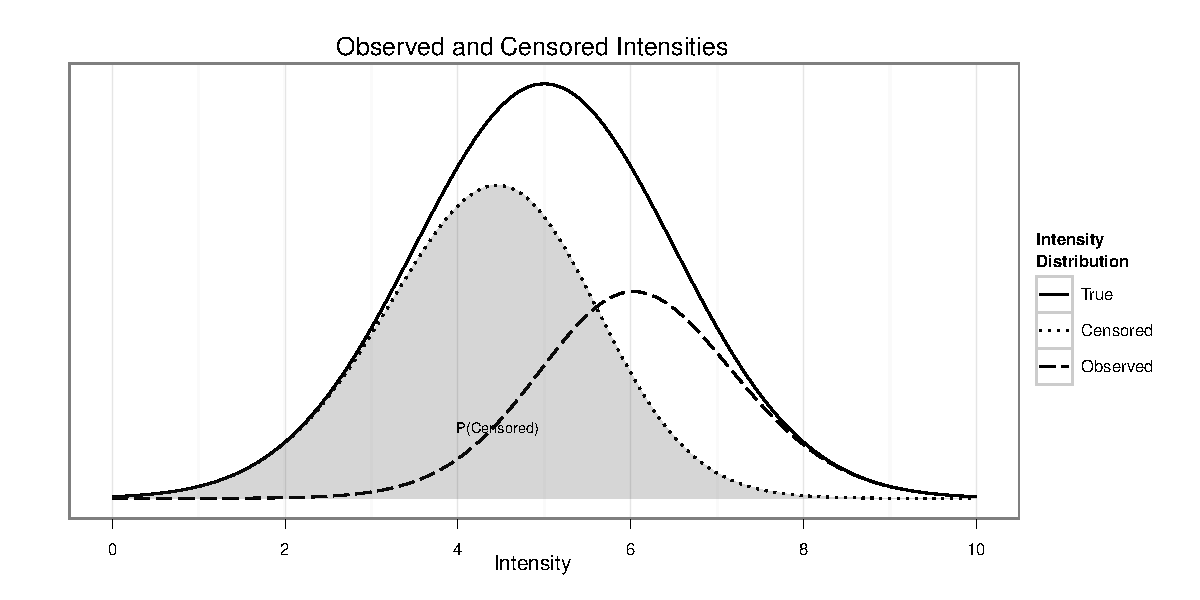
\includegraphics[width=0.8\textwidth]{figures/proteomics/Fig2_Observed_Censored_Intensity_Distributions}
\caption{Comparisons of original, censored, and observed intensity distributions. \label{proteomics:fig:Laplace_Halleys_Outline}}
\end{figure}

\begin{algorithm}[H]
\caption{N Censored Rejection Sampler\label{proteomics:alg:N-Censored-Rejection-Sampler-Algorithm}}

\begin{enumerate}
\item Draw $X\sim NegativeBinomial(1-\hat{p}_{ik}^{*},s_{ik}^{obs}+r)$, with $\hat{p}_{ik}^{*}=(1-\lambda)\left[\pi^{rnd}+(1-\pi^{rnd})\hat{\pi}_{ik}^{IC}\right]$
and $U\sim Uniform(0,1)$.
\item Accept $s_{ik}^{cen}=X$, if $U\leq\begin{cases}
\frac{(s_{ik}^{obs}+s_{ik}^{mis})}{(s_{ik}^{obs}+s_{ik}^{mis}+r-1)} & \text{if }r\geq1\\
\frac{(s_{ik}^{obs}+s_{ik}^{mis})}{s_{ik}^{obs}+s_{ik}^{mis}+r-1}\times\frac{s_{ik}^{obs}+r-1}{s_{ik}^{obs}} & \text{if }0<r<1
\end{cases}$.
\item Return to $1$ otherwise.\end{enumerate}
\end{algorithm}


\begin{figure}
\begin{center}
\includegraphics[width=.75\textwidth]{figures/proteomics/figure_nstates_sampler}
\end{center}
\caption{Expected iterations per accepted draw for $s_{ik}^{mis}$ rejection sampler for $\lambda=0.1$, $\pi^{rnd}=0.1$, and $\pi_{ik}^{IC}=.5$, with $r$ ranging from 0.5 to 5, $s_{ik}^{obs}$ ranging from 1 to 10. \label{proteomics:fig:s_ik^mis-Rejection-Sampler}}
\end{figure}


\subsubsection{Drawing from $p(\bm{R} \mid \bm s, \bm{Y}^{obs}, \bm{\Theta})$} \label{proteomics:sec:r_ik_mis_post}

After drawing the number of states per peptide $s_ik$, we draw the latent random censoring indicators for each censored peptide, $R_{ikl}^{mis}$.
Because random censoring occurs before intensity-based censoring, if a peptide was randomly censored ($R_{ikl}=0$), then $p(I_{ikl}=1\vert R_{ikl}=0,\bm{\Theta})=0$ and $p(O_{ikl}=1\vert R_{ikl}=0,\bm{\Theta})=0$ as outlined in Figure \ref{proteomics:fig:Missing_Data_Indicators_Tree}.
We then obtain the posterior probability that a peptide is randomly censored given that it is missing via a straightforward application of Bayes Theorem:
\begin{eqnarray}
p(R_{ikl}=1\vert O_{ikl}=0,\bm{\Theta}, \bm{Y}^{obs}) & = & 1 - \frac{p(O_{ikl}=0\vert R_{ikl}=0,\bm{\Theta}, \bm{Y}^{obs})p(R_{ikl}=0\vert\bm{\Theta}, \bm{Y}^{obs})}{\sum_{r_{ikl}=0}^{1}p(O_{ikl}=0\vert R_{ikl}=r_{ikl},\bm{\Theta})p(R_{ikl}=r_{ikl}\vert\bm{\Theta}, \bm{Y}^{obs})}\nonumber \\
% & = & \frac{1\times\pi^{rnd}}{\pi^{rnd}\times1+(1-\pi^{rnd})p(O_{ikl}=0\vert R_{ikl}=0,\bm{\Theta})}\label{proteomics:eq:w-posterior-in-text-1}\\
% & = & \frac{\pi^{rnd}}{\pi^{rnd}+(1-\pi^{rnd})\int_{-\infty}^{\infty}p(I_{ikl}=1\vert y_{ikl},R_{ikl}=0,\bm{\Theta})p(y_{ikl}\vert R_{ikl}=0,\bm{\Theta})dY_{ikl}} \label{proteomics:r-posterior}\\
 & = & 1 - \frac{\pi^{rnd}}{\pi^{rnd}+(1-\pi^{rnd})\pi_{ik}^{int}},
\end{eqnarray}
where $\pi_{ikl}^{int}$ is defined as in (\ref{proteomics:eqn:pi_IC}).
Plugging in our numerical approximation for $\pi_{ikl}^{int}$, $\hat{\pi}_{ikl}^{int}$, we draw
\begin{equation}
R_{ikl} \mid \bm{Y}^{obs}, \bm{\Theta}, s_{ik} \sim Bernoulli\left(1 - \frac{\pi^{rnd}}{\pi^{rnd}+(1-\pi^{rnd})\hat{\pi}_{ik}^{int}}\right) .
\end{equation}


\subsubsection{Drawing from $p(\bm{Y}^{mis} \mid \bm{R}, \bm{s}, \bm{Y}^{obs}, \bm{\Theta})$}
\label{proteomics:sec:y_ikl_mis_draw}

The final step in drawing the missing data is to impute the unobserved intensities by drawing each intensity from its full conditional posterior distribution.
The full conditional posterior is given by
\begin{eqnarray*}
p(y_{ikl}^{mis}\vert s_{ik}^{mis},R_{ik},\bm{\Theta}) & \propto & \begin{cases}
\phi\left(\frac{y_{ikl} - \gamma_{ik}}{\sigma_{i}}\right) & \text{if }R_{ikl}=0 \text{ and }O_{ikl}=0\\
\phi\left(\frac{y_{ikl} - \gamma_{ik}}{\sigma_{i}}\right) g(y_{ikl}, \bm \eta) & \text{if }R_{ikl}=1 \text{ and }O_{ikl}=0
\end{cases} .
\end{eqnarray*}
For randomly censored states, where $R_{ikl}=0$, the missingness mechanism is ignorable given $R_{ikl}$.
Hence, we simply draw $y_{ikl}^{mis}$ from its unconditional distribution,
\begin{eqnarray*}
p(y_{ikl}^{mis}\vert s_{ik}^{mis}, I_{ik}=0, R_{ikl}=0, \bm{\Theta}) & \sim & Normal(\gamma_{ik},\sigma_{i}^{2}).
\end{eqnarray*}
%
The posterior distribution for intensity-censored states ($R_{ikl}=1$, $I_{ikl}=0$) is given by
\begin{eqnarray}
p(y_{ikl}^{mis}\vert O_{ikl}=0,R_{ikl}=1,\bm{\Theta}) & = & (\pi_{ik}^{int})^{-1}\frac{1}{\sigma_{i}} \phi\left(\frac{y_{ikl}^{mis}-\gamma_{ik}}{\sigma_{i}}\right) g(y_{ikl}^{mis}, \bm \eta) .
\label{proteomics:eq:intensity-censored-posterior-text}
\end{eqnarray}
As this is not a standard distribution, we draw from it using a rejection sampler.
We use information from the adaptive quadrature of Section \ref{proteomics:sc:draw_s_ik_mis} to construct an efficient proposal distribution with little additional computation.
Specifically, we propose from a location-scale transformation of a $t_{\nu}$-distribution as
\begin{eqnarray}
Y_{ikl}^{*} & \sim & \hat{y}_{ikl}^{mis}+\hat{\sigma}_{ik}^{mis} \sqrt{\frac{\nu-2}{\nu}} t_{\nu},
\end{eqnarray}
which has expectation $\hat{y}_{ik}^{mis}$ and variance $\hat{\sigma}_{ik}^{mis})^{2}$ for $\nu>2$.

The rejection sampling algorithm requires bounding the ratio of the target density to the proposal density.
For this sampler, the given ratio has two local maxima, as shown in Figure \ref{proteomics:fig:Censored-Intensity-Rejection-Sampler-Outline-TEXT} B and C.
The global maximum of the ratio can be either the first or third root of the log-ratio's derivative depending upon the particular relationship between $\bm \eta$, $\sigma^2_i$, and $\gamma_ik$.
To reliably find the global maximum of the target-proposal density ratio, we use a pair of vectorized bisection searches to find the roots of the derivative of the log-ratio in two ranges: $(-\infty,\hat{y}_{ik}^{mis})$ and $(\hat{y}_{ik}^{mis},\infty)$.
Once these roots are obtained, we simply select the one corresponding to the larger local maximum to compute acceptance probabilities.
A graphical example of the rejection sampler is shown in Figure \ref{proteomics:fig:Censored-Intensity-Rejection-Sampler-Outline-TEXT} D, and the sampling algorithm is detailed in Algorithm \ref{proteomics:alg:Censored-Intensity-Accept-Reject-Algorithm-TEXT}.


\begin{comment}
\begin{eqnarray*}
X & \sim & t_{\nu}\\
y_{ikl}^{*} & \sim & \tilde{\sigma}_{ik}X+\tilde{\mu}_{ik}
\end{eqnarray*}
which has density, 
\begin{eqnarray}
g(y_{ikl}^{*}\vert\nu,\tilde{\mu}_{ikl},\tilde{\sigma}_{ikl}) & = & \frac{\Gamma\left(\frac{\nu+1}{2}\right)}{\sqrt{\nu\pi}\Gamma\left(\frac{\nu}{2}\right)}\left(1+\frac{(y_{ikl}^{*}-\tilde{\mu}_{ikl})^{2}}{\nu\tilde{\sigma}_{ikl}^{2}}\right)^{-\left(\frac{\nu+1}{2}\right)}\label{proteomics:eq:cen-int-proposal-density-TEXT}
\end{eqnarray}


, where
\begin{eqnarray*}
\tilde{\mu}_{ik} & \equiv & \underset{y_{ikl}^{mis}\in\mathbb{R}}{\arg\max}p(y_{ikl}^{mis}\vert I_{ikl}=0,W_{ikl}=0,\bm{\Theta})\\
\tilde{\sigma}_{ik}^{2} & \equiv & -\left(\frac{\partial^{2}}{\partial(y_{ikl}^{mis})^{2}}\log p(y_{ikl}^{mis}\vert I_{ikl}=0,W_{ikl}=0,\bm{\Theta})\right)^{-1}\Biggr|_{y_{ikl}^{mis}=\tilde{\mu}_{ik}}
\end{eqnarray*}
. These location and scale parameters correspond to the approximate
mean and variance used in the Laplace Approximation, see \subref{Drawing-n-cen-TEXT}.
This proposal is vastly more efficient than a proposal based on $y_{ikl}$
being $Normal(\gamma_{ik},\sigma_{i}^{2})$ at no additional computational
cost, since we need only to recognize the relation to the Laplace
Approximation. To use rejection sampling, we need to bound the targe-proposal
density ratio 
\begin{eqnarray}
\frac{p(y_{ikl}^{mis}\vert I_{ikl}=0,W_{ikl}=0,\bm{\Theta})}{g(y_{ikl}^{mis}\vert\nu,\tilde{\mu}_{ikl},\tilde{\sigma}_{ikl})} & \leq & z_{ikl}\label{proteomics:eq:cen int target-proposal ratio TEXT}
\end{eqnarray}
. However, this ratio isn't strictly concave, but bimodal with a mode
below and above $\tilde{\mu}_{ik}$; an example is shown in \figref{Censored-Intensity-Rejection-Sampler-Outline-TEXT}b.
We use a pair of bisection searches to find the roots of the first
derivative of the log target-proposal ratio, which is shown in \figref{Censored-Intensity-Rejection-Sampler-Outline-TEXT}c.
We are then able to obtain the global bound on the target-proposal
ratio and construct our rejection sampler from the posterior of the
censored intensities exactly. The rejection sampler is outlined in
\algref{Censored-Intensity-Accept-Reject-Algorithm} and depicted
in \figref{Censored-Intensity-Rejection-Sampler-Outline-TEXT} d.
\end{comment}


\begin{figure}
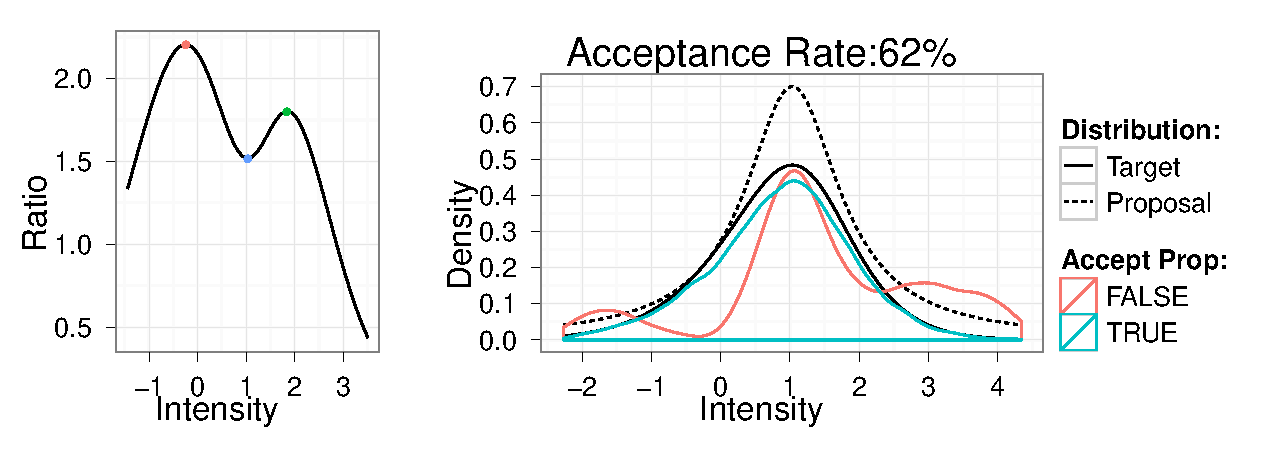
\includegraphics[width=1\textwidth]{figures/proteomics/figure_ycen_rejection_sampler.pdf}
\caption{Censored Intensity Rejection Sampler Example\label{proteomics:fig:Censored-Intensity-Rejection-Sampler-Outline-TEXT}}
\end{figure}


\begin{algorithm}
\caption{Censored Intensity Accept Reject Algorithm\label{proteomics:alg:Censored-Intensity-Accept-Reject-Algorithm-TEXT}}


$ $Target density: $f^{mis}(y_{ikl}\vert\eta_{0},\eta_{1},\gamma_{ik},\sigma_{i}^{2})=(\pi_{ik}^{int})^{-1} \frac{1}{\sigma_{i}}\phi\left(\frac{y_{ikl}-\gamma_{ik}}{\sigma_{i}}\right) g(y_{ikl}, \bm \eta)$.

Proposal density: $f^*(y_{ikl}^{*}\vert\nu,\tilde{\mu}_{ikl},\tilde{\sigma}_{ikl})=\frac{\Gamma\left(\frac{\nu+1}{2}\right)}{\sqrt{\nu\pi}\Gamma\left(\frac{\nu}{2}\right)}\left(1+\frac{(y_{ikl}^{*}-\tilde{\mu}_{ikl})^{2}}{\nu\tilde{\sigma}_{ikl}^{2}}\right)^{-\left(\frac{\nu+1}{2}\right)}$.
\begin{enumerate}
\item Compute $z_{ikl}$:

\begin{enumerate}
\item Using bisection, find the roots of of the first derivative of the
log density ratio, \\
$z_{ikl}^{(1)}\equiv\underset{y_{ikl}\in[-\infty,\tilde{\mu}_{ikl})}{\arg\max}\log\left[\frac{f^{mis}(y_{ikl}\vert\eta_{0},\eta_{1},\gamma_{ik},\sigma_{i}^{2})}{f^*(y_{ikl}\vert\nu,\tilde{\mu}_{ikl},\tilde{\sigma}_{ikl})}\right]$
and $z_{ikl}^{(2)}\equiv\underset{y_{ikl}\in(\tilde{\mu}_{ikl},\infty]}{\arg\max}\log\left[\frac{f^{mis}(y_{ikl}\vert\eta_{0},\eta_{1},\gamma_{ik},\sigma_{i}^{2})}{f^*(y_{ikl}\vert\nu,\tilde{\mu}_{ikl},\tilde{\sigma}_{ikl})}\right]$.
\item Determine the maximum of the density ratios,\\
 $c^* \equiv \max\left(\frac{f^{mis}(z_{ikl}^{(1)}\vert\eta_{0},\eta_{int},\gamma_{ik},\sigma_{i}^{2})}{f^*(z_{ikl}^{(1)}\vert\nu,\tilde{\mu}_{ikl},\tilde{\sigma}_{ikl})},\frac{f^{mis}(z_{ikl}^{(2)}\vert\eta_{0},\eta_{1},\gamma_{ik},\sigma_{i}^{2})}{f^*(z_{ikl}^{(2)}\vert\nu,\tilde{\mu}_{ikl},\tilde{\sigma}_{ikl})}\right)$.
\end{enumerate}
\item Generate $X\sim g(y_{ikl}^{*}\vert\nu,\tilde{\mu}_{ikl},\tilde{\sigma}_{ikl})$,
$U\sim Unif(0,1)$.
\item Accept $y_{ikl}=X$, if $U\leq\frac{f^{mis}(X\vert\eta_{0},\eta_{int},\gamma_{ik},\sigma_{i}^{2})}{c^* f^*(X\vert\nu,\tilde{\mu}_{ikl},\tilde{\sigma}_{ikl})}$.
\item Else, return to $2$.\end{enumerate}
\end{algorithm}


 %%% %%% %%%
 %%% %%% %%%


\section{Simulation studies}
\label{proteomics:sec:simulations}

To evaluate the performance of our method and the stability of the algorithm presented in Section \ref{proteomics:sec:estimation}, we tested our method on a set of simulated MS-MS experiments.
We describe the design of these simulations in detail in Section \ref{proteomics:sec:doe}.
We cover the computational performance and validation of our MCMC sampler in Section \ref{proteomics:sec:mcmc_performance}.
In Section \ref{proteomics:sec:frequentist_evaluations}, we evaluate the frequentist properties of our Bayesian estimates, including the coverage of our posterior intervals (\ref{proteomics:sec:coverage}) and the performance of the proposed method relative to standard estimators used for this class of experiments (\ref{proteomics:sec:compperf}).

 %%% %%% %%%
 %%% %%% %%%
 %%% %%% %%%

\subsection{Design of experiments}
\label{proteomics:sec:doe}

We simulated a set of complex biological samples, spanning a broad range of abundances and protein-specific properties.
For each such sample we simulate 54 proteins with abundances spanning 6 orders magnitude, $\mu_i= 3, \ldots, 8$, yielding 9 proteins per abundance level.
Within each abundance level, each simulated protein consists of $m_{ik}=20,25\ldots,60$ peptides.
With these properties fixed across replicates, we simulated 1,200 experiments from the model described in Section \ref{proteomics:sec:model}, using a probit link function for $g(\cdot, \bm \eta)$.
These consisted for 400 replicates for each of the parameter settings provided in Table \ref{proteomics:table:sim_parameters}, each of which was based on estimates from an experiment with the given gradient length using the Sigma UPS2 standard.

\begin{table}
\begin{center}
\caption{Parameter settings for simulation studies.
\label{proteomics:table:sim_parameters}}
\begin{tabular}{r|ccccccccc}
  \hline
Gradient & $\alpha_\tau$ & $\beta_\tau$ & $\alpha_\sigma$ & $\beta_\sigma$ & $\pi^{rnd}$ & $\eta_0$ & $\eta_1$ & $\lambda$ & $r$ \\ 
  \hline
   90m & 6.3 & 2.1 & 8.5 & 3.5 & 0.20 & 16 & -3.0 & 0.84 & 1.9 \\ 
  180m & 5.3 & 1.3 & 7.0 & 4.1 & 0.21 & 14 & -2.7 & 0.79 & 1.9 \\ 
  360m & 6.2 & 1.8 & 7.0 & 2.5 & 0.30 & 20 & -4.3 & 0.62 & 1.6 \\ 
   \hline
\end{tabular}
\end{center}
\end{table}

%Across these experiments, we fixed our top-level parameters to the following values: $\alpha_\tau=4$, $\beta_\tau=5$, $\alpha_\sigma=8$, $\beta_\sigma=4$, $\pi^{rnd}=0.1$, $\eta_0=-6.25$, $\eta_1=1.25$, $\lambda=0.1$, and $r=3$.


%% why these values? add a paragraph with some comments on the values; what observable properties they imply (e.g., 50% missing at .. and 10% missing at ..). how many state-level intensities (data points) on average in each data set?
%These values were selected based upon initial estimates from experiments using the Sigma UPS2 standard.
%They imply 50\% missingness at an intensity of $5.18$, 90\% missingness at an intensity of 3.34, and 15\% missingness at an intensity of 7.27.
%These also imply a mean of $1.33$ possible states per peptide with 99\% having between 1 and 4 possible states.
%The variance parameters yield $E[\sigma_i] = 1.39$ and $E[\tau_i] = 0.87$, with 95\% of their values within $(0.93, 1.90)$ and $(0.47, 1.32)$, respectively.
%These reflect a typical regime for both the missingness mechanism and the degree of variation observed in MS-MS data.


\subsection{MCMC performance and validation}
\label{proteomics:sec:mcmc_performance}

Our MCMC sampler produced high-quality draws from the target posterior at a low computational cost.
Running 3,000 iterations for each replicate required an average of 267 seconds (0.088 seconds per iteration) with a standard deviation of 17.1 seconds.
Of these 3,000 iterations, we discarded the first 1,000 as burn in.
The mean effective sample sizes for each top-level parameter based on the remaining 2,000 draws are provided in Table \ref{proteomics:tab:effective_sample_sizes}.
For $\mu_i$ and $\zeta_i$, we also include the mean standard deviation of effective sample sizes across proteins.
%
\begin{table}
\centering
\caption{Average effective sample sizes by parameter. $\pm$ for $\mu_{i}$
and $\zeta_{i}$ indicates the average standard deviation of effective
sample sizes across proteins. \label{proteomics:tab:effective_sample_sizes}}
\begin{tabular}{r|cccccccccc}
\hline 
Gradient  & $\zeta_{i}$ & $\eta$  & $\lambda$ & $\mu_i$  & $\pi^{rnd}$ & $r$ & $\beta_{\sigma}$ & $\beta_{\tau}$ & $\alpha_{\sigma}$ & $\alpha_{\tau}$\tabularnewline
\hline 
90m  & 341$\pm$188  & 287  & 773  & 331$\pm$191 & 191  & 1160  & 272  & 217  & 303  & 242 \tabularnewline
180m  & 256$\pm$143 & 285  & 823  & 250$\pm$148 & 175  & 1197  & 337  & 176  & 379  & 191 \tabularnewline
360m  & 421$\pm$208 & 179  & 1013  & 411 $\pm$215 & 275  & 1338  & 346  & 222  & 392  & 250 \tabularnewline
\hline 
\end{tabular}
\end{table}
%
We note that all mean effective sample sizes are greater than 100, indicating that even 2,000 iterations are sufficient to obtain Monte Carlo  an order of magnitude below the posterior standard deviation of each parameter.

\subsection{Frequentist evaluations}
\label{proteomics:sec:frequentist_evaluations}

\subsubsection{Coverage analysis}
\label{proteomics:sec:coverage}

We first used our simulated replicates to evaluate the frequency coverage of our posterior intervals, focusing on those for $\zeta_i$.
The results of these evaluations are summarized in Figure \ref{proteomics:fig:coverage_mu_hpd}; corresponding results for coverage vs. $m_i$ are similar and provided in Appendix \ref{ch:supp:proteomics}.
%
\begin{figure}
\centering
\includegraphics[width=\textwidth, page=1]{figures/proteomics/figures_coverage_sim}
\caption{Coverage of HPD intervals vs. $\mu_i$ by simulated gradient length and Bayesian level.
\label{proteomics:fig:coverage_mu_hpd}}
\end{figure}
%
We find that our posterior intervals are well-calibrated for the regimes of interest.
Across all three simulated gradient lengths, we obtain 67\% coverage for our 68\% posterior intervals, 89\% mean coverage for our 90\% posterior intervals, 94\% mean coverage for our 95\% posterior intervals, and 98\% mean coverage for our 99\% posterior intervals.
These demonstrate that, despite the complexity of our Bayesian method, it can provide inferences with frequentist guarantees.

%\begin{figure}
%\centering
%\includegraphics[width=\textwidth, page=3]{figures/proteomics/figures_coverage_sim}
%\caption{Coverage of HPD intervals vs. $m_i$ by simulated gradient length and Bayesian level.
%\label{proteomics:fig:coverage_mi_hpd}}
%\end{figure}

\subsubsection{Comparison with exiting methods}
\label{proteomics:sec:compperf}

We compared the performance of our model-based abundance estimates with several standard methods for absolute protein quantitation.
Many of these methods were originally developed for relative quantitation and are converted to absolute measures by appropriate rescaling.
All methods used in this comparison are of the form
\begin{equation}
 \hat{\zeta}_i = \log_{10}\left( \hat{T} \frac{10^{\hat{\mu}_i}}{\sum_i 10^{\hat{\mu}_i}} \right) .
\end{equation}
%
We compare the performance of our method to two classes of common methods: intensity-based estimators and count-based estimators.
We set $\hat{T} = \sum_i 10^{\mu_i}$ for all of these estimators.
Among intensity-based estimators, we consider simple summed intensities  (\ref{proteomics:eq:summed_intensity}) and median observed intensity  (\ref{proteomics:eq:median_intensity}) \citep[e.g.,][]{Cox:2008uu}.
We also evaluate two variants based on estimators from the spectral counting literature: mean observed intensity (\ref{proteomics:eq:mean_intensity}) and adjusted mean observed intensity (\ref{proteomics:eq:adj_mean_obs_intensity})
\begin{eqnarray}
\hat \mu_{i}^{si} &=& \log_{10} \left( \sum_{kl} 10^{y^{obs}_{ikl}} \right),
\label{proteomics:eq:summed_intensity} \\
\hat \mu_{i}^{med} &=& \text{Med}_{kl}(y_{ikl}),
\label{proteomics:eq:median_intensity} \\
\hat \mu_{i}^{mi} &=& \log_{10}\left( \sum_{kl} 10^{y^{obs}_{ikl}}/m_i^{obs} \right),
\label{proteomics:eq:mean_intensity} \\
\hat \mu_{i}^{ami} &=& \log_{10}\left( \sum_{kl} 10^{y^{obs}_{ikl}}/\sum_{k} s^{obs}_{ik} \right) .
\label{proteomics:eq:adj_mean_obs_intensity}
\end{eqnarray}
%
In the above, $m_i$ is the (known) number of possible peptides that are generated by digesting protein $i$ using a particular enzyme.

Another common approach, known as spectral counting, disregards the intensity measurements and uses counts of the observed states associated with each protein.
A range of such methods have been developed relative quantitation, including basic spectral counting \citep[e.g.,][]{Liu:2004hv}, average spectral counts \citep[e.g.,][]{Weiss:2010ik}, and the proportion of peptides identified (PPI) \citep{Rappsilber2002}.
However, these are not directly suitable for absolute quantitation due to a lack of normalization.
\citet{Ishihama:2005ir} defined an exponentially-modified protein abundance index (emPAI) to address these issues:
%
\begin{equation}
\hat \mu_{i}^{emPAI} = \log_{10}\left( 10^{\sum_k \mathbb{I}(s_{ik}^{obs} > 0) / m_i } - 1 \right) .
\label{proteomics:eq:empai}
\end{equation}
This provides a commonly-used representative of the count-based class of methods.

We summarize the results of these comparisons in Figures \ref{proteomics:fig:compare_relative_error} and \ref{proteomics:fig:compare_bias}.
%
\begin{figure}
\centering
\includegraphics[width=\textwidth, page=3]{figures/proteomics/figures_relative_error_sim}
\caption{Relative efficiency of standard methods ($MSE_{Method} / MSE_{Model-based}$) vs. $\mu_i$ and $m_i$ by block (left and right columns, respectively). Relative MSE axis is logarithmic. Solid black line at 1 corresponds to the model-based method's efficiency, by definition.
\label{proteomics:fig:compare_relative_error}}
\end{figure}
%
Complete tabular results are available in Appendix \ref{ch:supp:proteomics}.
From Figure \ref{proteomics:fig:compare_relative_error}, we see that our method reduces the overall MSE of abundance estimates by a factor of 5--10 relative to intensity-based estimates and by a factor of 6--150 relative to emPAI.
Most intensity-based estimators exhibit consistent efficiency relative to ours, although the median intensity estimator's efficiency improves to nearly 1 as abundance increases.
However, this estimator's efficiency is quite poor for low-abundance proteins with approximately 20 times the model-based estimator's MSE.
The efficiency of emPAI increases by an order of magnitude over the range of simulated abundances and decreases slightly with protein length $m_i$, demonstrating the value of intensity information in low-abundance regimes.
By carefully combining count and intensity information, we obtain consistent reductions in MSE relative to both classes of methods for all values of $\mu_i$ and $m_i$.

\begin{figure}
\centering
\includegraphics[width=\textwidth, page=3]{figures/proteomics/figures_bias_sim}
\caption{Bias of $\hat{\zeta}_i$ for standard methods and posterior mean from model vs. $\mu_i$ and $m_i$ by gradient length (left and right columns, respectively).
\label{proteomics:fig:compare_bias}}
\end{figure}
%
Turning to bias, we see that the model-based estimator provides lower bias than both classes of standard methods.
Summed intensity shows a slight negative bias (between -0.7 and 0), while mean and average mean observed intensity show a positive bias of similar magnitude.
The median intensity estimator shows a far larger positive bias (nearly 2 orders of magnitude) at low abundances.
The biases of all four intensity-based estimators diminish as abundance increases.
The emPAI estimator shows a large positive bias that also decreases in magnitude with abundance.
The bias of the summed intensity estimator diminishes from approximately -0.7 to 0 as protein length increases; the biases of our other estimators exhibits little sensitivity to protein length.
Again, we see that our model-based approach enables us to combine count and intensity information into estimators that outperform both classes of standard methods.

 %%% %%% %%%
 %%% %%% %%%


\section{Empirical results}
\label{proteomics:sec:empirical}

Having established our method's properties on simulated data, we turn to actual experimental data.
We use a quantitative protein standard, described in Section \ref{proteomics:sec:data}, for these experiments.
This standard provides known abundances for evaluation with a realistic set of proteins.
In Section \ref{proteomics:sec:checkassumptions}, we use these experiments to check our model assumptions and demonstrate their implications for real data.
In Section \ref{proteomics:sec:dataanalysis}, we assess the comparative performance of the proposed methods with respect to the standard methods presented in Section \ref{proteomics:sec:compperf}.

 %%% %%% %%%
 %%% %%% %%%

\subsection{Data}
\label{proteomics:sec:data}

We conducted a set of LC/MS-MS experiments using the Universal Proteome Standard 2 (UPS2), a constructed biological sample that contains 48 human proteins.
These proteins are present in six concentrations, ranging from .5fM to 50,000 fM, with eight known proteins at each concentration.
These proteins are selected to span a broad range of physical properties (size and hydrophobicity) within each concentration, removing a potential confounding factor while reflecting the actual variation among proteins in typical samples.
The concentration specified for each protein in the standard was confirmed by the manufacturer using multiple methods, so we are comfortable taking the concentrations reported by the manufacturer as ground truth for subsequent analyses.
With its high dynamic range, the standard provides a realistic and stringent test of our method.

We ran five LC/MS-MS experiments using this standard at three gradient lengths, 90, 180, and 360 minutes, with two, two, and one replicates per gradient length, respectively.
Each gradient length implies a different set of parameters for the missing data mechanism.
Longer gradients allow for the observation of a greater variety MS2 spectra and is expected to decrease the degree of intensity-based missingness.
However, longer gradients can also reduce the dynamic range of observed intensities and require substantially greater effort from the experimenter.
Our experiments allow us to explore these tradeoffs in as we evaluate our method.
The 90 minute gradients reflect the degree of censoring typically observed in analyses of more complex mixtures, while the 180 and 360 minute gradients provide a ``sanity check'' of our method's behavior in a setting with less missing data.

 %%% %%% %%%
 %%% %%% %%%

\subsection{Exploratory analysis and model checking}
\label{proteomics:sec:checkassumptions}

Using the experimental data, we examined the distributions of intensities, identifications, and states to check the assumptions of our model.
Figure \ref{proteomics:fig:EDA-Figure} summarizes these results.
%
\begin{figure}
\centering
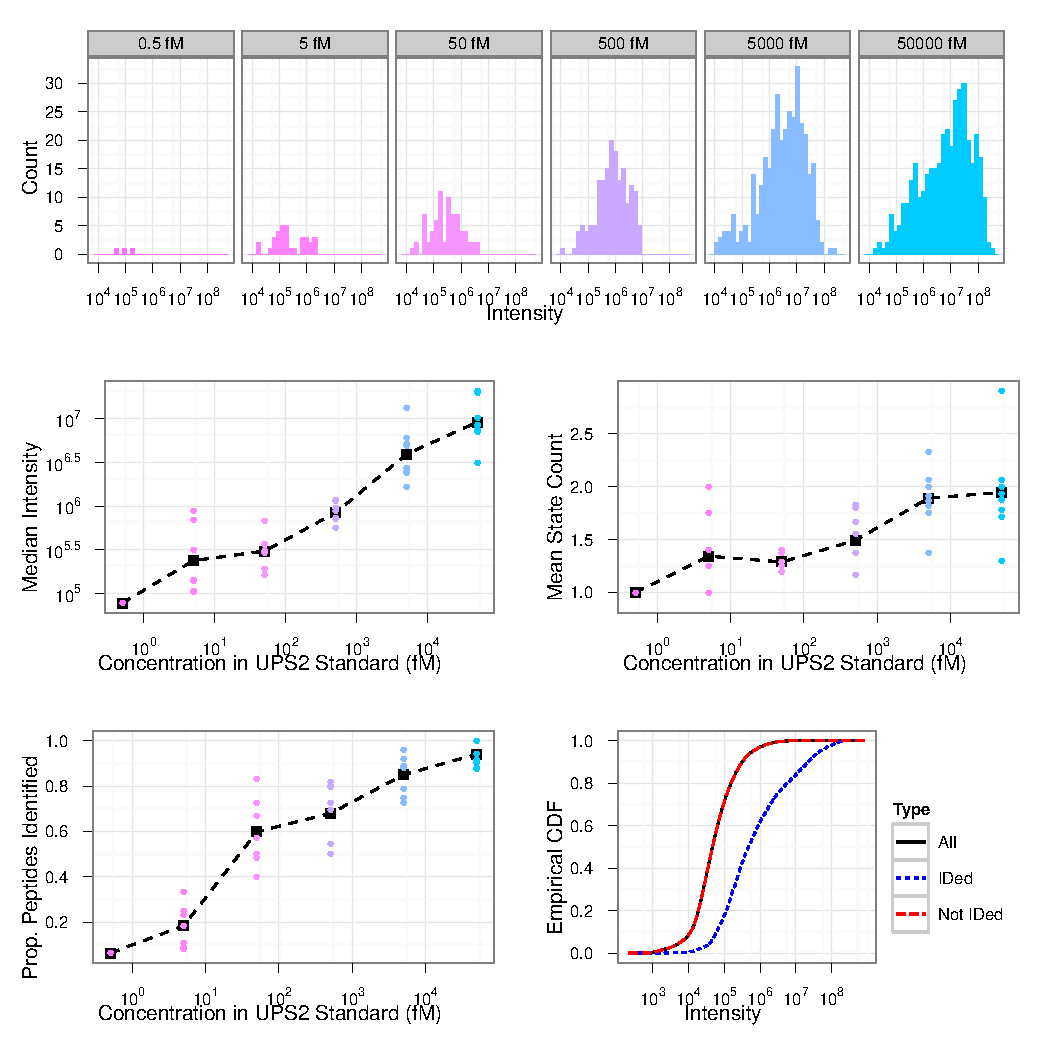
\includegraphics[width=\textwidth]{figures/proteomics/New_EDA_Multipanel_Figure}
\caption{Exploratory data analysis using the UPS2 quantitative protein standard.
\label{proteomics:fig:EDA-Figure}}
\end{figure}
%
Panel A of this figure shows the observed distribution of intensities by concentration.
It is immediately clear from these histograms that the number of intensities observed and the median observed intensity increases strongly with the concentration.
The distributions of observed intensities are also right-skewed for each concentration level, which is consistent with the combination of intensity-dependent censoring and an underlying log-normal distribution of intensities.

Panels B, C, and D show the relationship between concentration and identification, median intensity, and $s_{ik}^{obs}$ in greater detail.
The median observed intensity by protein increases with the protein's concentration, although the former has far less dynamic range than the latter (2 orders of magnitude vs. 5).
Intensity-based censoring at the state level explains this discrepancy, as the lowest-intensity ions are preferentially removed from the sample.
%
We also compared the number of states that peptides were detected in across protein concentrations.
The physical process that generates distinct peptide states is known to be independent of protein or peptide abundance, so the number of \emph{possible} peptide states must be invariant to the peptide's concentration.
Since it is not possible to determine the number of possible states per for peptide \emph{a priori}, we model this value as an IID random variable in our model.
However, we observe a strong relationship between the number of observed peptide states and concentration in the experimental data.
This supports the assumption of intensity-dependent state-level censoring in our model.

The proportion of peptides identified per protein ranges nearly 1 for the most abundant proteins to approximately 5\% for the least abundant, while the 
This is mostly attributable to selection for abundant ions within the MS-MS equipment, as panel E demonstrates.
By design, the subset of peptides selected for fragmentation is determined by the instrument's software in real time as the sample is analyzed.
While we focus on the subset of peptides that are both detected by the mass spectrometer and successfully identified, nearly all of the peptides in the sample can be quantified in terms of their total intensity\footnote{
Software is able to quantify peptides that were not identified is due to the both mass accuracy of the mass spectrometer and the effective separation of the sample by chromatography.
The software used to process the experimental data \citep{Cox:2008uu} is able to identify and integrate over all unique profiles in the m/z $\times$ intensity $\times$ retention time space, as shown in Figure \ref{proteomics:fig:Mass_Spec_Overview} C.
This allows quantitation of the majority of peptides; however, since the majority of these are not identified, there is no way to map them to a specific protein.
Hence, we exclude them from our model-based inference.}.
This allows us to investigate the intensity-dependence of the peptide identification process in detail and validate our model assumptions.
Comparing the distributions of identified and unidentified state-level intensities in Panel E shows that (1) the distribution of identified intensities stochastically dominates that of the unidentified intensities and (2) there is substantial overlap between these distributions.
(1) is consistent with Theorem \ref{proteomics:thm:dominance}, while (2) is consistent with the assumption of a stochastic censoring mechanism.

 %%% %%% %%%
 %%% %%% %%%

\subsection{Comparison of empirical results}
\label{proteomics:sec:dataanalysis}

We used the experiments described in Section \ref{proteomics:sec:data} to evaluate our method's performance against the standard methods described in Section \ref{proteomics:sec:compperf}.
We summarize these results in Figure \ref{proteomics:fig:UPS2 results} and Table \ref{proteomics:tab:UPS2 results} and provide complete tables of results in Appendix \ref{ch:supp:proteomics}.
%
\begin{figure}
\centering
\includegraphics[width=\textwidth]{figures/proteomics/figures_draft_ups2}
\caption{Inferred protein abundances from experiments with UPS2 standard.
\label{proteomics:fig:UPS2 results}}
\end{figure}
%
\begin{table}
\centering
\caption{Mean squared errors $\pm$ standard errors from experiments with UPS2 standard.
\label{proteomics:tab:UPS2 results}}
%\begin{tabular}{l|ccccc}
%  \hline
%Gradient & Posterior mean & Summed intensity & Mean obs. intensity & Median intensity & emPAI \\ 
%  \hline
%90m & $0.41 \pm 0.11$ & $1.06 \pm 0.12$ & $2.45 \pm 0.16$ & $3.18 \pm 0.13$ & $2.81 \pm 0.10$ \\ 
%  180m & $0.34 \pm 0.07$ & $0.76 \pm 0.14$ & $1.82 \pm 0.21$ & $2.26 \pm 0.21$ & $3.03 \pm 0.12$ \\ 
%  360m & $0.37 \pm 0.06$ & $0.65 \pm 0.07$ & $1.26 \pm 0.08$ & $1.87 \pm 0.06$ & $3.55 \pm 0.13$ \\ 
%   \hline
%\end{tabular}
\begin{tabular}{l|ccc}
\hline
& \multicolumn{3}{c}{Gradient length} \\
  \hline
Method & 90m & 180m & 360m \\ 
  \hline
Posterior mean & $0.41 \pm 0.11$ & $0.34 \pm 0.07$ & $0.37 \pm 0.06$ \\ 
  Summed intensity & $1.06 \pm 0.12$ & $0.76 \pm 0.14$ & $0.65 \pm 0.07$ \\ 
  Mean obs. intensity & $2.45 \pm 0.16$ & $1.82 \pm 0.21$ & $1.26 \pm 0.08$ \\ 
  Median intensity & $3.18 \pm 0.13$ & $2.26 \pm 0.21$ & $1.87 \pm 0.06$ \\ 
  emPAI & $2.81 \pm 0.10$ & $3.03 \pm 0.12$ & $3.55 \pm 0.13$ \\ 
   \hline
\end{tabular}
\end{table}
%
We restrict our attention here to the best-performing subset of the estimators presented in Section \ref{proteomics:sec:compperf}.
We see from Table \ref{proteomics:tab:UPS2 results} that our method's performance is particularly strong on short gradients, providing a factor of 2.6 reduction in MSE relative to the best standard estimator (summed intensity) for the 90 minute gradients and a factor of 2.2 reduction for the 180 minute gradients.
On the longest gradient (360 minutes), our method's MSE is a factor of 1.8 lower than than that of the best standard estimator.
This behavior matches our expectations based on the relevant properties of the underlying experimental processes.
Detailed modeling of the missing data mechanism yields the largest gains when the sample is least separated and there are fewer possible spectra---in the shortest gradients.
In the longest gradient, intensity-based missingness diminishes in importance relative to other factors.

From Figure \ref{proteomics:fig:UPS2 results}, we note that our method's improvements are greatest for low-abundance proteins.
All estimators considered provide reasonably good estimates of $\zeta_i$ for the highest-abundance proteins.
However, most of the standard estimators exhibit a substantial positive bias (1-2 orders of magnitude) for the lowest-abundance proteins, particularly on short gradients.
In contrast, our method provides consistently accurate estimates for low-abundance proteins across all gradient lengths.
We discuss the implications of this capability for biological applications in Section \ref{proteomics:sec:remarks}.
%However, the mean intensity estimator appears to perform better on this measure.
%This estimator implicitly imputes zeros for all unobserved peptide intensities by using the number of predicted peptides $m_i$ as a denominator, correcting for some of the positive bias in observed intensities.
%This implicit correction is not sufficient to yield accurate results on the shorter gradients, though.



 %%% %%% %%%
 %%% %%% %%%

\section{Concluding remarks}
\label{proteomics:sec:remarks}

We have presented a model-based approach to label-free absolute quantitation in LC/MS-MS proteomics experiments.
As the results of Sections \ref{proteomics:sec:simulations} and \ref{proteomics:sec:empirical} show, accounting for non-ignorable missing data in the proteomics context improves estimates of absolute abundances.
Our method also provides well-calibrated measures of uncertainty, as the results of Sections \ref{proteomics:sec:coverage} and \ref{proteomics:sec:dataanalysis} show.
Below, we provide some broader context and particular insights on this class of methods and problems, focusing on the role of non-ignorable missing data in complex experiments, efficient computation with missing data of variable dimension, and the role of absolute quantitation in biological analyses.
We also discussion extensions of the methods presented to the semi-supervised setting and distributed computational environments.

\subsection{Modeling and inference}

The core of our model for LC-MS/MS proteomics data is the structure of our non-ignorable missing data mechanism.
We explicitly account for the dependence of censoring probabilities on unobserved peptide intensities at the level of individual peptide states.
This creates an additional complication, as the number of possible states per peptide is unknown.
Thus, we must account for truncation at the state level in addition to censoring at the peptide level.
However, we do know that the distribution of then number possible peptide states is invariant to the peptide's concentration.
Incorporating this information into our model allows us to extract information from the number of states observed per peptide ($s_{ik}^{obs}$).

Working with state-level data provides fine-grained measures of missingness, which provide a great deal of information on low-abundance proteins when used properly.
For high-abundance proteins, the vast majority of peptide states are observed, providing the majority of the information on the underlying distribution of the number of states per peptides.
Our model uses this information to improve inferences on the abundances of low-abundance proteins, leveraging all of the available information from their intensity and state information.
Extracting all of this information requires a sophisticated approach to inference and computation, however.

The presence of state-level censoring with an unknown number of states per peptide makes inference under our missing data model particularly challenging.
The dimension of our missing data $\bm M$ varies across draws, requiring more specialized computational strategies than standard Metropolis-Hastings updates.
We implemented an exact marginal draw from the conditional distribution of $\bm M$ given $\bm \Theta$ using a combination of unidimensional numerical integration and efficient rejection sampling, as detailed in Section \ref{proteomics:sec:missingDataDraw}.
The reductions in autocorrelation provided by this marginal update more than offset the computational costs of rejection sampling and numerical approximation.
This allows for efficient inference in the presence of missing data of unknown dimension, as the results of Section \ref{proteomics:sec:simulations} demonstrate.
We believe that this technique can provide effective computational techniques for a range of non-ignorable missing data problems originating from complex experimental techniques.

\subsection{Applications}

Absolute quantitation provides a different view on biological processes than relative quantitation, enabling the study of new phenomena.
Whereas relative quantitation can only measure the protein-by-protein differences in abundances across experiments, absolute quantitation provides estimates of the abundances of different proteins within a single population of cells.
Such information is somewhat interesting for high-abundance proteins, but it promises the greatest insights from the study of low-abundance ones.

Reliable, accurate quantitation of low-abundance proteins also makes LC/MS-MS methods applicable to new classes of biological investigations.
Two of the most promising areas are the study of mistranslation and transcription factors.
Both involve proteins which appear at low concentrations but can have an outsized biological impact.
In the case of mistranslation, the cell must spend a great deal of energy handling defective proteins; the rate of mistranslation represents the largest determinant of these costs.
Transcription factors regulate the conversion of DNA into mRNA, providing one of the primary mechanisms of control and feedback for cellular functions.
Our method allows for reliable estimates of these proteins' concentrations within large populations of cells, opening new areas for high-throughput research.

\subsection{Extensions}

We are developing two extensions of the proposed methodology with a focus on larger, shallower datasets.
In relatively shallow datasets, few proteins are observed and, due to intensity-based censoring, the dynamic range of observed intensities is compressed.
This makes estimation of the censoring parameters ($\eta$ and $\pi^{rnd}$) from observed data difficult, reducing the precision of our estimates.
The quantitative protein standard described in Section \ref{proteomics:sec:data} provides a potential solution to this problem.
Such a standard can be spiked into the biological sample of interest and used as a calibration source.
A semi-supervised version of the model presented in Section \ref{proteomics:sec:model} can use the known properties of this standard to enable reliable inferences about the censoring mechanism in shallow samples.
As an additional benefit, this supervision could simplify the conversion of our estimates between the intensity and abundance scales.

To tackle larger datasets, including full-proteome quantitation for complex organisms, we are also developing a distributed variant of the MCMC algorithm presented here.
The goal is to scale the sampler across computational clusters with minimal communication within iterations.
The conditional independence structure of the model presented in Section \ref{proteomics:sec:model} makes such distribution both appealing and feasible.

We see a rich range of opportunities for statistical research in this area.
The field of MS-MS proteomics is young, and it can provide a unique view on the details of biological processes.
Extracting this technology's full value requires care, deep subject-matter knowledge, and sophisticated statistical techniques, but the rewards are great.
We hope that more statisticians will enter this field and continue to build strong methodological foundations to advance biological research.

 %%% %%% %%%
 %%% %%% %%%
 %%% %%% %%%

\section{Acknowledgments}

This work was partially supported by the National Science Foundation under grants no.\ DMS-0907009 and no.\ IIS-1017967, by the National Institute of Health under grant no.\ R01 GM-096193, all to Harvard University. Additional funding was provided by the Harvard Medical School's Milton Fund.
%%
%The views and conclusions contained in this document are those of the  authors and should not be interpreted as representing the official policies, either expressed or implied, of the National Institute of Health, the Army Research Office, the National Science Foundation, or the U.S. government.

 %%% %%% %%%
 %%% %%% %%%
 %%% %%% %%%

%\appendix

\section{Proof of Theorem \ref{proteomics:thm:dominance}}

\begin{proof}
Define $Y$ as a random variable with a distribution given by
%
\begin{equation}
\nonumber
\dd F_Y(y) = \frac{1}{w} g(y) \dd F_x(y)
\end{equation}
%
where $w \equiv \int_{\Reals} g(t) \dd F_x(t) \equiv P(Z=1)$. We assume we are in a non-trivial case, so $w \in (0,1)$.
%
Then, define $h \equiv g^{-1}(w)$. Consider the difference $D(t) \equiv F_X(t) - F_Y(t)$. This difference is equivalent to
%
\begin{equation}
\nonumber
D(t) = \int_{\Reals} \left(1 - \frac{1}{w}g(x) \right) \dd F_X(x)
\end{equation}
%
We now consider two cases:
\begin{enumerate}
\item[(1)] If $t \leq h$, then we have $g(x) \leq w$ for all $x \in (-\infty, h])$ by monotonicity. Thus, over the same range, $\left(1 - \frac{1}{w}g(x) \right) \geq 0$, so $D(t) \geq 0$.

\item[(2)] If $t > h$, then
%
\begin{equation}
\nonumber
D(t) = \int_{-\infty}^h \left(1 - \frac{1}{w}g(x) \right) \dd F_X(x) + 
	\int_{h}^t \left(1 - \frac{1}{w}g(x) \right) \dd F_X(x)
\end{equation}
%
Now, we have $D(h) \geq 0$ from case (1) and we know $D(h) \rightarrow 0$ as $t \rightarrow \infty$ as it is the difference of CDFs. By monotonicity, for $x \geq h$, $g(x) \geq w$, so $1 - \frac{1}{w}g(x) \leq 0$ for $x \in [h,t]$. Thus, as $\dd F_X(x) \geq 0$, we know that $\int_{h}^t \left(1 - \frac{1}{w}g(x)\right) \dd F_X(x)$ is (weakly) monotone decreasing in $t$ and $\leq 0$. Thus, $D(t)$ increases monotonically to $D(h)$, then decreases monotonically to zero from $h$ as $t \rightarrow \infty$.
\end{enumerate}
%
Therefore, for any value of $t$, we have shown that $D(t) \geq 0$. Thus, $Y$ stochastically dominates $X$.

\end{proof}

%!TEX TS-program = xelatex
% !TEX root = ../thesis.tex
% Do not delete; used to set build system

\begin{savequote}[75mm] 
Nulla facilisi. In vel sem. Morbi id urna in diam dignissim feugiat. Proin molestie tortor eu velit. Aliquam erat volutpat. Nullam ultrices, diam tempus vulputate egestas, eros pede varius leo.
\qauthor{Quoteauthor Lastname} 
\end{savequote}

\chapter{The promise and perils of preprocessing: building foundations for multiphase inference}

\section{Summary}

Preprocessing forms an oft-neglected foundation for a wide range of statistical and scientific analyses.
However, it is rife with subtleties and pitfalls.
Decisions made in preprocessing constrain all later analyses and are typically irreversible.
Hence, data analysis becomes a collaborative endeavor by all parties involved in data collection, preprocessing and curation, and downstream inference.
Even if each party has done its best given the information and resources available to them, the final result may still fall short of the best possible in the traditional single-phase inference framework.
This is particularly relevant as we enter the era of ``big data''.
The technologies driving this data explosion are subject to complex new forms of measurement error.
Simultaneously, we are accumulating increasingly massive databases of scientific analyses.
As a result, preprocessing has become more vital (and potentially more dangerous) than ever before.

We propose a theoretical framework for the analysis of preprocessing under the banner of multiphase inference.
We provide some initial theoretical foundations for this area, including distributed preprocessing, building upon previous work in multiple imputation.
We motivate this foundation with two problems from biology and astrophysics, illustrating multiphase pitfalls and potential solutions.
These examples also emphasize the motivations behind multiphase analyses---both practical and theoretical.
We demonstrate that multiphase inferences can, in some cases, even surpass standard single-phase estimators in efficiency and robustness.
Our work suggests several rich paths for further research into the statistical principles underlying preprocessing.
%
%Our work highlights the importance of providing information beyond ``optimal''
%estimators for downstream analyses.
%
To tackle our increasingly complex and massive data, we must ensure that our inferences are built upon solid inputs and sound principles.
Principled investigation of preprocessing is thus a vital direction for statistical research.

\section{What is multiphase inference?}

\subsection{Defining multiphase problems}
Preprocessing and the analysis of preprocessed data are ubiquitous components of statistical analysis, but their treatment has often been informal.
We aim to develop a theory that provides a set of formal statistical principles for such problems under the banner of multiphase inference.
The term ``multiphase'' refers to settings in which inferences are obtained through the application of multiple procedures in sequence, with each procedure taking the output of the previous phase as its input.
This encompasses settings such as multiple imputation \citep[MI,][]{Rubin1987} and extends to other situations.
In a multiphase setting, information can be passed between phases in an arbitrary form; it need not consist of (independent) draws from a posterior predictive distribution, as is typical with multiple imputation.
Moreover, the analysis procedure for subsequent phases is not constrained to a particular recipe, such as Rubin's MI combining rules \citep{Rubin1987}.

The practice of multiphase inference is currently widespread in applied statistics.
It is widely used as an analysis technique within single publications---any paper that uses a ``pipeline'' to obtain its final inputs or clusters derived estimates provides an example.
Furthermore, projects in astronomy, biology, ecology, and social sciences (to name a small sampling) increasingly focus on building databases for future analyses as a primary objective.
These projects must decide what levels of preprocessing to apply to their data and what additional information to provide to their users.
Providing all of the original data clearly allows the most flexibility in subsequent analyses.
In practice, the journey from raw data to a complete model is typically too intricate and problematic for the majority of users, who instead choose to use preprocessed output.

Unfortunately, decisions made at this stage can be  quite treacherous. Preprocessing is typically irreversible, necessitating assumptions about both the observation mechanism and future analyses. These assumptions constrain all subsequent analyses.
Consequently, improper processing can cause a disproportionate amount of damage to a whole body of statistical results.
However, preprocessing can be a powerful tool.
It alleviates complexity for downstream researchers, allowing them to deal with smaller inputs and (hopefully) less intricate models.
This can provide large mental and computational savings.

Two examples of such trade-offs come from NASA and high-throughput biology.
When NASA satellites collect readings, the raw data are usually massive.
These raw data are referred to as the ``Level 0'' data \citep{ChandraSDP}.
The Level 0 data are rarely used directly for scientific analyses.
Instead, it is processed to Levels 1, 2, and 3, each of which involves a greater degree of reduction and adjustment.
Level 2 is typically the point at which the processing becomes irreversible.
\cite{Braverman2012} provide an excellent illustration of this process for the Atmospheric Infrared Sounder (AIRS) experiment.
This processing can be quite controversial within the astronomical community.
Several upcoming projects, such as the Advanced Technology Solar Telescope (ATST) will not be able to retain the Level 0 or Level 1 data \citep{Davey2012}.
This inability to obtain raw data and increased dependence on preprocessing has transformed low-level technical issues of calibration and reduction into a pressing concern.

High-throughput biology faces similar challenges.
Whereas reproducibility is much needed \citep[e.g. ][]{Ioannidis2011}, sharing raw datasets is difficult because of their sizes.
The situation within each analysis is similar.
Confronted with an overwhelming onslaught of raw data, extensive preprocessing has become crucial and ubiquitous.
Complex models for genomic, proteomic, and transcriptomic data are usually built upon these heavily-processed inputs.
This has made the intricate details of observation models and the corresponding preprocessing steps the groundwork for entire fields.

To many statisticians, this setting presents something of a conundrum.
After all, the ideal inference and prediction will generally use a complete correctly-specified model encompassing the underlying process of interest and all observation processes.
Then, why are we interested in multiphase?
We focus on settings where there is a natural separation of knowledge between analysts, which translates into a separation of effort.
The first analyst(s) involved in preprocessing often have better knowledge of the observation model than those performing subsequent analyses.
For example, the first analyst may have detailed knowledge of the structure of experimental errors, the equipment used, or the particulars of various protocols.
This knowledge may not be easy to encapsulate for later analysts---the relevant information may be too large or complex, or the methods required to exploit this information in subsequent analyses may be prohibitively intricate.
%
% As mentioned previously, such cases are ubiquitous across many scientific fields.
%
Hence, the practical objective in such settings is to enable the best possible inference given the constraints imposed and provide an account of the tradeoffs and dangers involved.
To borrow the phrasing of \citet{Meng2003} and \citet{Rubin1996}, we aim for achievable practical efficiency rather than a theoretical efficiency that is practically unattainable.

Multiphase inference currently represents a serious gap between statistical theory and practice.
We typically delineate between the informal work of preprocessing and feature engineering and formal, theoretically-motivated work of estimation, testing, and so forth.
However, the former fundamentally constrains what the latter can accomplish.
As a result, we believe that it represents a great challenge and opportunity to build new statistical foundations to inform statistical practice.

\subsection{Practical motivations}
\label{multiphase:sec:examples}

We present two examples  that show both the impetus for and perils of undertaking multiphase analyses in place of inference with a complete, joint model. The first concerns  microarrays,  which allow the analysis of thousands of genes in parallel.
We focus on expression microarrays, which measure the level of gene expression in populations of cells based upon the concentration of RNA from different genes.
These are typically used to study changes in gene expression between different experimental conditions.

In such studies, the estimand of interest is typically the log-fold change in gene expression between conditions.
However, the raw data consist only of intensity measurements for each probe on the array, which are grouped by gene along with some form of controls.
These intensities are subject to several forms of observation noise, including additive background variation and additional forms of interprobe and interchip variation (typically modeled as multiplicative noise).
To deal with these forms of observation noise, a wide range of background correction and normalization strategies have been developed \citep[for a sampling, see][]{Tusher2001,Quackenbush2002,Affymetrix2002,Irizarry2003,McGee2006,Ritchie2007,Xie2009}.
Later analyses then focus on the scientific question of interest without, for the most part, addressing the underlying details of the observation mechanism.

Background correction is a particularly crucial step in this process, as it is typically the point at which the analysis moves from the original intensity scale to the log-transformed scale.
As a result, it can have a large effect on subsequent inferences about log-fold changes, especially for genes with low expression levels in one condition \citep{Smyth2005,Irizarry2006}.
One common method (MAS5),  provided by one microarray manufacturer, uses a combination of background subtraction and truncation at a fixed lower threshold for this task \citep{Affymetrix2002}. Other more sophisticated techniques use explicit probability models for this de-convolution.
A model with normally-distributed background variation and exponentially distributed expression levels has proven to be the most popular in this field \citep{McGee2006,Xie2009}.

Unfortunately, even the most sophisticated available techniques pass only point estimates onto downstream analyses.
This necessitates ad-hoc screening and corrections in subsequent analyses, especially when searching for significant changes in expression \citep[e.g.][]{Tusher2001}.
Retaining more information from the preprocessing phases of these analyses would allow for better, simpler inference techniques with greater power and fewer hacks.
The motivation behind the current approach is quite understandable: scientific investigators want to focus on their processes of interest without becoming entangled in the low-level details of observation mechanisms.
Nevertheless, this separation can clearly compromise the validity of their results.

The role of preprocessing in microarray studies extends well beyond background correction.
Normalization of expression levels across arrays, screening for data corruption, and other transformations preceding formal analysis are standard.
Each technique can dramatically affect downstream analyses.
For instance, quantile normalization equates quantiles of expression distributions between arrays, removing a considerable amount of information.
This mutes systematic errors \citep{Bolstad2003}, but it can seriously compromise analyses in certain contexts (e.g. miRNA studies).

Another example of multiphase inference can be found in the estimation of correlations based upon indirect measurements.
This appears in many fields, but astrophysics provides one recent and striking case.
The relationships between the dust's density, spectral properties, and temperature are of interest in studies of star-forming dust clouds.
These characteristics shed light on the mechanisms underlying star formation and other astronomical processes.
Several studies \citep[e.g.][]{Dupac2003,Desert2008,Anderson2010,Paradis2010} have investigated these relationships, finding negative correlations between the dust's temperature and spectral index.
This finding is counter to previous astrophysical theory, but it has inspired many alternative explanations.

Such investigations may, however, be chasing a phantasm.
These correlations have been estimated by simply correlating point estimates of the relevant quantities (temperature $T$ and spectral index $\beta$) based on a single set of underlying observations.
As a result, they may conflate properties of this estimation procedure with the underlying physical mechanisms of interest.
This has been noted in the field by \citet{Shetty2009}, but the scientific debate on this topic continues.
\cite{Kelly2012} provide a particularly strong argument, using a cohesive hierarchical Bayesian approach, that improper multiphase analyses have been a pervasive issue in this setting.
Improper preprocessing led to incorrect, negative estimates of the correlation between temperature and spectral index, according to \cite{Kelly2012}.
These incorrect estimates even appeared statistically significant with narrow confidence intervals based on standard methods.
On a broader level, this case again demonstrates some of the dangers of multiphase analyses when they are not carried out properly.
Those analyzing this data followed an intuitive strategy: estimate what we want to work with ($T$ and $\beta$), then use it to estimate the relationship of interest.
Unfortunately, such intuition is not a recipe for valid statistical inference.%, as we shall demonstrate in this paper.

\subsection{Related work}

Multiphase inference has wide-ranging connections to both the theoretical and applied literatures.
It is intimately related to previous work on multiple imputation and missing data \citep{Rubin1976,Rubin1987,Meng1994,Rubin1996,Meng2003,Xie2012}.
In general, the problem of multiphase inference can be formulated as one of missing data.
However, in the multiphase setting, missingness arises from the preprocessing choices made, not a probabilistic response mechanism.
Thus, we can leverage the mathematical and computational methods of this literature, but many of its conceptual tools need to be modified.
Multiple imputation addresses many of the same issues as multiphase inference and is indeed a special case of the latter.
Concepts such as congeniality between imputation and analysis models and self-efficiency \citep{Meng1994} have natural analogues and roles to play in the analysis of multiphase inference problems.

Multiphase inference is also tightly connected to work on the comparison of experiments and approximate sufficiency, going back to \citet{Blackwell51,Blackwell53} and continuing through \citet{LeCam1964} and \citet{Goel79}, among others.
This literature has addressed the relationship between decision properties and the probabilistic structure of experiments, the relationship between different notions of statistical information, and notions of approximate sufficiency---all of these are quite relevant for the study of multiphase inference.
We view the multiphase setting as an extension of this work to address a broader range of real-world problems, as we will discuss in Section~\ref{multiphase:sec:riskmonotone}.

The literature on Bayesian combinations of experts also informs our thinking on multiphase procedures.
\citet{Kadane1993} provides an excellent review of the field, while \citet{Lindley1979} provides the core formalisms of interest for the multiphase setting.
Overall, this literature has focused on obtaining coherent (or otherwise favorable) decision rules when combining information from multiple Bayesian agents.
This line of work fits nicely into a multiphase framework, providing a rich body of theory upon which to build.
However, our focus is more sequential and mechanical than that of this literature.
The literature on combining Bayesian inferences has focused on the process of combining information in the form of multiple posterior distributions.
We view this as a best-case scenario, focusing our theoretical development towards the mechanics of passing information between phases.
We also focus on the sequential nature of multiphase settings and the challenges this brings for both preprocessors and downstream analysts, in contrast to the more ``parallel'' or simultaneous focus of the literature mentioned above.

There are also fascinating links between multiphase inference and the signal processing literature.
There has been extensive research on the design of quantizers and other compression systems \citep{Gray1998}.
Such work is often focused on practical questions, but it has also yielded some remarkable theory.
In particular, the work of \citet{Nguyen2009} on the relationship between surrogate loss functions in quantizer design and $f$-divergences suggests possible ways to develop and analyze a wide class of multiphase procedures, as we shall discuss  in Section \ref{multiphase:sec:future}.  

\section{Multiphase logic and concepts for preprocessing}
\label{multiphase:sec:concepts}

\subsection{A model for two phases}
\label{multiphase:sec:model}

To formalize the notion of multiphase inference, we begin with a formal model for two-phase settings.
The first phase consists of the data generation, collection, and preprocessing, while the second phase consists of inference using the first phase's output.
We will call the first-phase agent the ``preprocessor'' and the second-phase agent the ``downstream analyst''.
The preprocessor observes the raw data $Y$.
This is a noisy realization of $X$, variables of interest that are not directly obtainable from a given experiment, e.g., gene expression from sequencing data, or stellar intensity from telescopic observations.

We assume that the joint density of $X$ and $Y$ can be factored as 
\begin{equation}\label{multiphase:e:model}
 p_{Y,X}(Y,X \given \param, \obsparam) = \pobs(Y \given X, \param, \obsparam) \cdot\psci(X \given \param, \obsparam) = \pobs(Y \given X, \obsparam) \cdot \psci(X \given \param) \ .
\end{equation}
Here, $\psci$ encapsulates the underlying process of interest and $\pobs$ encapsulates the observation process.
We assume that $\param$ is of fixed dimension in all asymptotic settings.
In practice, the preprocessor should be able to postulate a reasonable ``observation model'' $\pobs(Y \given X, \obsparam)$, but will not always know the true ``scientific model'' $\psci(X \given \param)$.
This is analogous to the MI setting, where the imputer does not know the form of the final analysis.

Using this model, the preprocessor provides the downstream analyst with some output $T = T(Y, U)$, where $U$ is a (possibly stochastic) additional input.
When $T(Y, U)$ is stochastic (e.g., an MCMC output), the conditional distribution $\pproc(T|Y)$ plays a pivotal role in this process. For simplicity, we will present our results treating $T$ as a deterministic function of $Y$ only, but many results generalize easily.
Given such $T$, downstream analysts can carry out their inference procedures.
These procedures  need not correspond to inference under any  complete-data model, but they are typically  straightforward to formulate and evaluate.
We summarize the structure of this model in Figure \ref{multiphase:fig:models}.

\begin{figure}
\centering
\includegraphics[height=2in]{figures/multiphase/diagram_model_vertical}
\caption{Graphical diagram of our  generic two-phase setting. The preprocessor  observes $Y$ from the original data generating process and outputs $T$, with $X$ as missing data. The downstream analyst observes the preprocessor's output $T$ and has both $X$ and $Y$ missing.\label{multiphase:fig:models}}
\end{figure}

This model incorporates several restrictions.
First, it is Markovian with respect to $Y$, $X$, and $\param$; $Y$ is conditionally independent of $\param$ given $X$ (and $\obsparam$).
Second, the parameters governing the observation process ($\obsparam$) and those governing the scientific process  ($\param$) are distinct.
In Bayesian settings, we further assume that $\obsparam$ and $\param$ are independent \textit{a priori}.
The parameters $\obsparam$ are nuisance from the perspective of all involved; the downstream analyst wants to draw inferences about $X$ and $\param$, and the preprocessor wants to pass forward information that will be useful for said inferences.
If downstream inferences are Bayesian with respect to $\obsparam$, then $\pobs(Y|X) = \int \pobs(Y | X, \obsparam) \pi_\obsparam(\obsparam)\dd\mu_{\obsparam}(\obsparam)$ (which holds under (\ref{multiphase:e:model})) is sufficient for all inference under the given model and prior.
Hence, this conditional density is frequently of interest in our theoretical development, as is the corresponding marginalized model $p_{X,Y}(Y, X | \param) = \int \pobs(Y | X, \obsparam)  \psci(X | \param) \pi_\obsparam(\obsparam)\dd \mu_{\obsparam}(\obsparam)$.
We will compare results obtained with a fixed prior to those obtained in a more general setting to better understand the effects of nuisance parameters in multiphase inference.

These restrictions are somewhat similar to those underlying Rubin's definition of ``missing at random'' \citeyearpar{Rubin1976}; however, we do not have missing data mechanism (MDM) in this setting \emph{per se}.
The distinction between missing and observed data ($X$ and $Y$) is fixed by the structure of our model.
In place of MDM, we have two imposed patterns of missingness: one for the data-generating process, and one for the inference process.
The first is $\pobs(Y \given X, \obsparam)$, which creates a noisy version of the desired scientific variables.
Here, $X$ can be considered the missing data and $Y$ the observed.
For the inference process, the downstream analyst observes $T$ in place of $Y$ but desires inference for $\param$ based upon $\psci(X | \param)$.
Hence, $Y$ and $X$ are both missing for the downstream analyst.
Neither pattern is entirely intrinsic to the problem---both are fixed by choice.
The selection of scientific variables $X$ for a given marginal likelihood $\pobs(Y | \param, \obsparam) = \int \pobs(Y | X, \obsparam) \psci(X | \param) \dd X$ is a modeling decision.
The selection of preprocessing $T(Y, U)$ is fundamentally a design decision.
This contrasts with the typical missing data setting, where MDM is forced upon the analyst by nature.
With multiphase problems, we seek to design and evaluate engineered missingness.
The investigation of multiphase inference therefore requires tools and ideas from design, inference, and computation in addition to the theory of missing data.

\subsection{Defining multiphase procedures}
\label{multiphase:sec:def}

With this model in place, we turn to formally defining multiphase procedures.
This is more subtle than it initially appears.
In the MI setting, we focus on complete-data procedures for the downstream analyst's estimation and do not restrict the dependence structure between missing data and observations.
In contrast, we restrict the dependence structure as in (\ref{multiphase:e:model}), but place far fewer constraints on the analysts' procedures.

In our multiphase setting, downstream analysts need not have any complete-data procedure in the sense of one for inferring $\param$ from $X$ and $Y$; indeed, they need not formally have one based only upon $X$ for inferring $\param$.
We require only that they have a set of procedures for their desired inference using the quantities provided from earlier phases as inputs ($T$),  not necessarily  using direct observations of $X$ or $Y$.
Such situations are common in practice, as methods are often built around properties of preprocessed data such as smoothness or sparsity that need not hold for the actual values of $X$.

For the preprocessor, the input  is $Y$ and the output is $T$.
 Here  $T$ could consist of a vector of means with corresponding standard errors, or,  for discrete $Y$, $T$ could consist of carefully selected cross-tabulations.
In general, $T$ clearly needs to be related to $X$ to capture inferential information, but its actual form is influenced by practical constraints (e.g. aggregation to lower than desired resolutions due to data storage capacity).

For the downstream analyst, the input is $T$ and the output is an inference for $\theta$. 
They can obviously adapt. 
For example, suppose $\param = E(X_i)$ for each entry $i$ of $X$.
If they are given $T_0 = \hat{X}$, they may simply use an unweighted mean to estimate $\param$.
If they have $T_1 = (\hat{X}, S)$, where $S$ contains standard errors, they could instead use a weighted mean to estimate $\param$.
This adaptation extends to an arbitrary number of possible inputs $T_k$, each of which corresponds to a set of constraints facing the preprocessor.

To formalize this notion of adaptation, we first define an index set $C$ with one entry for each such set of constraints.
This maps between forms of input provided by the preprocessor and estimators selected by the downstream analyst.
In this way, $C$ captures the downstream analyst's knowledge of previous processing and the underlying probability model.
Thus, this index set plays an central role in the definition of multiphase inference problems, far beyond that of a mere mathematical formality; it defines the amount of mutual knowledge shared between the preprocessor and the downstream analyst.

Now, we turn to the estimators themselves.
We start with point estimation as a foundation for a broader class of problems.
Testing begins with estimating rejection regions, interval estimation with estimating coverage, classification with estimating class membership, and prediction with estimating future observations and, frequently, intermediate parameters.
The framework we present therefore provides tools that can be adapted for more than estimation theory.
We define multiphase estimation procedures as follows:
%
\begin{definition}
A \emph{multiphase estimation procedure} $\proc$ is a set of estimators $\{\est_k(T_k) : k \in C \}$ indexed by the set $C$, where $T_k$ corresponds to the output of the $k$th first-phase method; that is, $\proc$ is a family of estimators with different inputs.
\end{definition}
%
When clear, we will drop the subscripts $k$ and simply index the estimators in $\proc$ by their inputs.
This definition provides enough flexibility to capture many practical issues with multiphase inference.
It also encompasses the traditional definition of a missing data procedure used by \citet{Meng1994}, providing another link to that body of theory.
Such procedures cannot, of course, be arbitrarily constructed if they are to deliver results with general validity.
Hence, having defined these procedures, we will cull many of them from consideration in Section \ref{multiphase:sec:riskmonotone}.

The obvious choice of our estimand (suggested by our notation thus far) is the parameter for the scientific model, $\param$.
This is very amenable to mathematical analysis and relevant to many investigations.
Hence, it forms the basis for our results in Section \ref{multiphase:sec:theory}.
However, for multiphase analyses, other classes of estimands may prove more useful in practice.
In particular, functions of $X$, future scientific variables $X_{rep}$, or future observations $Y_{rep}$ may be of interest.
Prediction of such quantities is a natural focus in the multiphase setting because such statements are meaningful to both the preprocessor and downstream analyst.
% Statements about future observations $Y_{rep}$ and latent quantities $X$ then have the same meaning to both analysts.
Such estimands naturally encompass a broad range of statistical problems including prediction, classification, and clustering.
However, there is often a lack of mutual knowledge about $\psci(X \given \param)$, so the preprocessor cannot expect to ``target'' estimation of $\param$ in general, as we shall discuss in Section \ref{multiphase:sec:remarks}.


\subsection{When is more better?}
\label{multiphase:sec:riskmonotone}

It is not automatic for multiphase estimation procedures to produce better results as the first phase provides more information.
To obtain a sensible context for theoretical development, we must regulate the way that the downstream analyst adapts to different inputs.
For instance, they should obtain better results (in some sense) when provided with higher-resolution information.
This carries over from the MI  setting \citep{Meng1994,Meng2003,Meng2012,Xie2012}, where notions such as self-efficiency are useful for regulating the downstream analyst's procedures.
We define a similar property for multiphase estimation procedures, but without restricting  ourselves to the missing data setting. 
Specifically, let $T_1 \preceq T_2$ indicate $T_1$ is a deterministic function of $T_2$.
In practice, $T_1$ could be a subvector, aggregation, or other summary of $T_2$.
%
\begin{definition}[Risk monotonicity]
A multiphase estimation procedure $\proc$ is \emph{risk monotone} with respect to a loss function $L$ if, for all pairs of outputs $T_1, T_2$ $T_1 \preceq T_2$ implies $R(\est_2(T_2), L) \leq R(\est_1(T_1), L)$.
\end{definition}
%
An asymptotic analogue of risk monotonicity is defined as would be expected, scaling the relevant risks at an appropriate rate to obtain nontrivial limits.
This is a natural starting point for regulating multiphase estimation procedures; stronger notions may be required for certain theoretical results.
Note that this definition does not require that ``higher-quality'' inputs necessarily lead to lower risk estimators.
Risk monotonicity requires only that estimators based upon a larger set of inputs perform no worse than those with strictly less information (in a deterministic sense).
However, risk monotonicity is actually quite tight in another sense.
It requires that additional information cannot be misused by the downstream analyst, imposing a strong constraint on mutual knowledge.
For an example, consider the case of unweighted and weighted means.
To obtain better results when presented with standard errors, the downstream analyst must know that they are being given (the correct) standard errors and to weight by inverse variances.

This definition is related the comparison of experiments, as explored by \citet{Blackwell51,Blackwell53}, but diverges on a fundamental level.
Our ordering of experiments, based on deterministic functions, is more stringent than that of \cite{Blackwell53}, but they are related.
Indeed, our $\preceq$ relation implies that of \citet{Blackwell53}.
In the latter work, an experiment $\alpha$ is defined as more informative than experiment $\beta$, denoted $\alpha \supset \beta$, if all losses attainable from $\beta$ are also attainable from $\alpha$.
This relation is also implied if $\alpha$ is sufficient for $\beta$.
Our stringency stems for our broader objectives in the multiphase setting.
From a decision-theoretic perspective, the partial ordering of experiments investigated by Blackwell and others deal with which risks are attainable given pairs of experiments, allowing for arbitrary decision procedures.
In contrast, our criterion restricts procedures based on whether such risks are actually attained, with respect to a particular loss function.
This is because, in the multiphase setting, it is not generally realistic to expect downstream analysts to be capable of obtaining optimal estimators for all forms of preprocessing.

The conceptually-simplest way to generate such a procedure is to begin with a complete probability model for $\pobs(Y | \param)$.
Under traditional asymptotic regimes, all procedures consisting of Bayes estimators based upon such a model will (with full knowledge of the transformations involved in each $T_k$ and a fixed prior) be risk monotone.
The same is true under the same regimes (for squared-error loss) for procedures consisting of MLEs under a fixed model.
Under some other asymptotic regimes, however, these principles of estimation do not guarantee risk-monotonicity; we explore this further in Section \ref{multiphase:sec:missinfo}.
But such techniques are not the only way to generate risk monotone procedures from probability models.
This is analogous to self-efficiency, which can be achieved by procedures that are neither Bayesian nor MLE \citep{Meng1994,Xie2012}.

\begin{figure}
\centering
\includegraphics[height=1in]{figures/multiphase/diagram_risk-monotone.eps}
\caption{Illustration of risk-monotone ``basis'' construction. In this case, $T_1$ and $T_2$ for the basis set of statistics. Each of these has three descendants ($T_3, T_5, T_7$ from $T_1$ and $T_4, T_6, T_8$ from $T_2$). These descendants are deterministic functions of their parent, but they are not deterministic functions of any other basis statistics. Given correctly-specified models for $T_1$ and $T_2$, a risk monotone procedure can be constructed for all statistics ($T_1, \ldots, T_8$) shown here as described in the text.
\label{multiphase:fig:risk-monotone}}
\end{figure}

A risk monotone procedure can be generated from any set of probability models for distinct inputs that ``span'' the space of possible inputs.
Suppose that an analyst has a set of probability models, all correctly specified, for $p_{T_b}(T_b | \param)$, where $b$ ranges over a subset $B$ of the relevant index set $C$.
We also assume that this analyst has a prior distribution $\pi_b(\param)$ for each such basis models.
These priors need not agree between models; the analyst can build a risk-monotone procedure from an inconsistent set of prior beliefs.
Suppose that the inputs $\{T_b : b \in B\}$ are not deterministic functions of each other and all other inputs can be generated as nontrivial deterministic transformations of one of these inputs.
Formally, we require $T_b \not \preceq T_c$ for all distinct $b, c \in B$ and, for each $k \in C$ there exists a unique $b \in B$ such that $T_k \preceq T_b$ (each output is uniquely descended from a single $T_b$),
as illustrated  in Figure \ref{multiphase:fig:risk-monotone}.
This set can form a basis, in a sense, for the given procedure.

Using the given probability models with a single loss function and set of priors (potentially different for each model), the analyst can derive a Bayes rule under each model.
For each $b \in B$, we require $\est(T_b)$ to be an appropriate Bayes rule on said model.
As $T_k = g_k(T_b)$ for some function $g_k$, we then have the implied $p_{T_k}(T_k | \param) = \int_{t : g_k(t) = T_k} p_{T_b}(t | \param) \dd t$, yielding the Bayes rule for estimating $\param$  based on $T_k$, which is no less risky than $\est(T_b)$.
The requirement that each output $T_k$ derives from a unique $T_b$ means that each basis component $T_b$ has a unique line of descendants.
Within each line, each descendant is comparable to only a single $T_b$ in the sense of deterministic dependence.
Between these lines, such comparisons are not possible.
This ensures  the overall risk-monotonicity.

Biology provides an illustration of such bases.
A wide array of methodological approaches have been used to analyze high-throughput gene expression data.
One approach, builds upon order and rank statistics \citep{Geman2004,Tan2005,Geman2012}.
Another common approach uses differences in gene expression between conditions or experiments, often aggregating over pathways, replicates, and so forth.
Each class of methods is based upon a different form of preprocessing: ranks transformations for the former, normalization and aggregation for the latter.
Taking procedures based on rank statistics and aggregate differences in expression as a basis, we can consider constructing a risk-monotone procedure as above.
Thus, the given formulation can bring together apparently disparate methods as a first step in analyzing their multiphase properties.

Such constructions are, unfortunately, not sufficient to generate all possible risk monotone procedures.
Obtaining more general conditions and constructions for risk monotone procedures is a topic for further work.

\subsection{Revisiting our examples and probing our boundaries}
\label{multiphase:sec:revisit}

By casting the examples in Section \ref{multiphase:sec:examples} into the formal structure just established, we can clarify the practical role of each mathematical component and see how to map theoretical results into applied guidance.
We also provide an example  that illustrates the boundaries of the framework's utility, and another that demonstrates its formal limits.
These provide perspective on the tradeoffs made in formalizing the multiphase inference problem. 

The case of microarray preprocessing presented previously fits quite nicely into the model of Section \ref{multiphase:sec:model}.
There, $Y$ corresponds to the observed probe-level intensities, $X$ corresponds to the true expression level for each gene under each condition, and $\param$ corresponds to the parameters governing the organism's patterns of gene expression.
In the microarray setting, $\pobs$ would characterize the relationship between expression levels and observed intensities, governed by $\obsparam$.
These nuisance parameters could include chip-level offsets, properties of any additive background, and the magnitudes of other sources of variation.
The assumptions of a Markovian dependence structure and distinct parameters for each part of the model appear quite reasonable in this case, as (1) the observation $Y$ can only (physically) depend upon the sample preparation, experimental protocol, and RNA concentrations in the sample and (2) the distributions $\psci$ and $\pobs$ capture physically distinct portions of the experiment.
Background correction, normalization, and the reduction of observations to log-fold changes are common examples of preprocessing $T(Y)$. As discussed previously, estimands based upon $X$ may be of greater scientific than those based upon $\param$.
For instance, we may want to know  whether gene expression changed between two treatments in a particular experiment (a statement about $X$) than whether a parameter regulating the overall patterns of gene expression takes on a particular value.

For the astrophysical example, the fit is similarly tidy.
The raw astronomical observations correspond to $Y$, the true temperature, density, and spectral properties of each part each dust cloud become $X$, and the parameters governing the relationship between these quantities (e.g.
their correlation) form $\param$.
The $\pobs$ distribution governs the physical observation process, controlled by $\obsparam$.
This process typically includes the instruments' response to astronomical signals, atmospheric distortions, and other earthbound phenomena.
As before, the conditional independence of $\param$ and $Y$ given $X$ and $\obsparam$ is sensible based upon the problem's structure, as is the separation of $\param$ and $\obsparam$. Here  $X$ corresponds to signals emitted billions or trillions of miles from Earth, whereas the observation process occurs within ground- or space-based telescopes.
Hence, any non-Markovian effects are quite implausible.
Preprocessing $T(Y)$ corresponds to the (point) estimates of temperature, density, and spectral properties from simple models of $Y$ given $X$ and $\obsparam$.

The multiphase framework encompasses a broad range of settings, but it does not shed additional light on all of them.
If $T$ is a many-to-one transformation of $Y$, then our framework implies that the preprocessor and downstream analyst face fundamentally different inference (and missing data) problems.
This is the essence of multiphase inference, in our view.
Settings where $\pobs(Y|X, \obsparam)$ is degenerate or $T$ is a one-to-one function of $Y$ are boundary cases where our multiphase interpretation and framework add little.

For a concrete example of these cases, consider a time-to-failure experiment, with the times of failure $W_i \sim \,\mbox{i.i.d}\, \Expo(\param)$, $i = 1, \ldots, n$.
Now, suppose that the experimenters actually ran the experiment in $m$ equally-sized batches.
They observe each batch only until its first failure; that is, they observe and report $Y_b = \min \{W_i : i \mbox{ in batch } b \}$ for each batch $b$.
Subsequent analysts have access only to $T = (Y_1, \ldots, Y_b)$.
This seems to be a case of preprocessing, but it actually resides at the very edge of our framework.

We could take the complete observations to be $X$ and the batch minima to be $Y$.
This would satisfy our Markov constraint, with a singular, and hence deterministic, observation process $\pobs(Y | X)$ simply selecting a particular order statistic within each batch.
However, $T(Y)$ is one-to-one; the preprocessor observes only the order statistics, as does the downstream analyst.
There is no separation of inference between phases; the same quantities are observed and missing to both the preprocessor and the downstream analyst.
Squeezing this case into the multiphase framework is technically valid but unproductive.

The framework we present is not, however, completely generic.
To find an example entirely beyond the boundaries of the given model, we must consider the Markov property and the separation of scientific and observation parameters ($\param$ and $\obsparam$).
Consider a chemical experiment involving a set of reactions.
The underlying parameters $\param$ describe the chemical properties driving the reactions, $X$ are the actual states of the reaction, and $Y$ are the (indirectly) measured outputs of the reactions.
The measurement process for these experiments, as described by $\pobs(Y|X, \obsparam)$, could easily violate the structure of our model in this case.
For instance, the same chemical parameters could affect both the measurement and reaction processes, violating the assumed separation of $\param$ and $\obsparam$.

Even careful preprocessing in such a setting can create a fundamental incoherence.
Suppose the downstream analysis will be Bayesian, so the preprocessor provides the conditional density of $Y$ as a function of $X$, $\pobs(Y | X)$,  for the observed $Y$.
If $\param$ and $\obsparam$ share components, and the preprocessor uses their prior on $\obsparam$ to create $\pobs(Y | X)$, the conditional density need not be sufficient for $\param$ under the downstream analyst's model.
Because the downstream analyst's prior on $\param$ need not be compatible with the preprocessor's prior on $\obsparam$, inferences based on the preprocessor's $\pobs(Y | X)$ can be seriously flawed in this setting.
Hence, we exclude such cases from our investigation for the time being.

Our model also excludes cases where the downstream analyst has better access to observations than the preprocessor.
That is, the downstream analyst cannot have access to $X$ itself or any other output less noisy than $Y$.
This removes from consideration, for instance, cases where the preprocessor and downstream analyst simply have access to different outputs from the same experiments.
Their data must follow the given conditional independence structure for us to view the setting as preprocessing, with the preprocessor's output providing the downstream analyst's only window on the experiment of interest.

We do not exclude cases where the downstream analyst has more knowledge about $\param$ than the preprocessor.
However, it does severely restrict the form such information can take---it must be conditionally independent of the scientific variables $X$ and observations $Y$ given $(\param, \obsparam)$ or $\param$.
For example, the downstream analyst could observe completely separate experiments pertaining to the same underlying process (governed by $\param$) or the outcomes of separate calibration (pertaining to $\obsparam$), but not additional replicates governed by the same realization of $X$.
In a biological setting, this means that the downstream analyst could have access to results from samples not available to the preprocessor (e.g. biological replicates), possibly using the same equipment; however, they could not have access to additional analyses of the same biological sample (e.g. technical replicates), as a single biological sample would typically correspond to a single realization of $X$.

These examples remind us that our multiphase setting does not encompass all of statistical inference.
This is quite a relief to us.
Our work aims to open new directions for statistical research, but it does not attempt address every problem under the sun!

\subsection{Constraints will set your theory free}
\label{multiphase:sec:constraints}

Multiphase theory hinges on procedural constraints.
Consider, for example, finding the optimal multiphase estimation procedure in terms of the final estimator's Bayes risk.
Without stringent procedural constraints, the result is trivial: compute the appropriate Bayes estimator using the distribution of $T$ given $\param$.
Similarly, the optimal preprocessing $T$ will, without tight constraints, simply compute an optimal estimator using $Y$ and pass it forward.
Note that both of these cases respect risk-monotonicity to the letter; it is not sufficiently tight to enable interesting, relevant theory.
% This pattern repeats across many inquiries, with both Bayesian, frequentist, and asymptotic techniques and for both phases.
More constraints, based upon careful consideration of applied problems, are clearly required.

This is not altogether bad news.
We need only look to the history of multiple imputation to see how rich theory can arise from stringent, pragmatic constraints.
Multiple imputation is a narrow class of multiphase procedures: all $T's$ usually consist of posterior predictive draws of $X$, and the second-phase procedure can only repeatedly apply a complete-data procedure and combine the results.
These constraints were originally imposed for practical reasons---in particular, to make the resulting procedure feasible with existing software.
However, they have opened the door to deep theoretical investigations.

In that spirit, we consider two types of practically-motivated constraints for multiphase inference: restrictions on the downstream analyst's procedure and restrictions on the preprocessor's methods.
These constraints are intended to work in concert with coherence conditions (e.g. risk monotonicity), not in isolation, to enable meaningful theory.

Constraints on the downstream analyst are intended to reflect practical limitations of their analytic capacity.
Examples of this type include restricting the downstream analyst to narrow classes of estimators (e.g. linear functions of preprocessed inputs), to specific principles of estimation (e.g. MLEs), or to special cases of a method we can reasonably assume the downstream analyst could handle, such as a complete-data estimator $\est(X)$, available from  a software with appropriate inputs.
Estimators derived from nested families of models are often suitable for this purpose.
For example, whereas $\est(X)$ may only involve an  ordinary  regression, the computation of  $\est(T)$ may require  a weighted least-squares regression.
%This is an example of  constructing  a reasonably constrained procedure, specializing a feasible estimator to generate a wide family of options.
% All of these constraints can rule out many forms of adaptation, enabling richer theory.

Another constraint on the downstream analyst pertains to nuisance parameters.
Such constraints are of great practical and theoretical interest, as we believe that the preprocessor will typically have better knowledge and statistical resources available to address nuisance parameters than the downstream analyst.
An extreme (but realistic) case of this is to assume that the downstream analyst cannot address nuisance parameters at all.
As we shall discuss in Section \ref{multiphase:sec:theory}, this would force the preprocessor to either marginalize over the nuisance parameters, find a pivot with respect to them, or trust the downstream analyst to use a method robust to the problematic parameters.

Turning to the preprocessor, we consider restricting either the form of the preprocessor's output or the mechanics of their methods.
In the simplest case of the former, we could require that $T$ consist of $X$'s posterior mean ($\hat{X}$) and posterior covariance ($V$) under the preprocessor's model.
A richer, but still realistic, class of output would be finite-dimensional real or integer vectors.
Restricting output to such a class would prevent the preprocessor from passing arbitrary function onto the downstream analyst.
This leads naturally to the investigation of (finite-dimensional) approximations to the preprocessor's conditional density, aggregation, and other such techniques.

On the mechanical side, we can restrict either the particulars of the preprocessor's methods or their broader properties.
Examples of the former include particular computational approximations to the likelihood function or restrictions to particular principles of inference (e.g. summaries of the likelihood or posterior distribution of $X$ given $(Y, \obsparam)$).
Such can focus our inquiries to specific, feasible methods of interest or reflect the core statistical principles we believe the preprocessor should take into account.
In a different vein, we can require that preprocessor's procedures be distributable across multiple researchers, each with their own experiments and scientific variables of interest.
Such settings are of interest for both the accumulation of scientific results for later use and the development of distributed statistical computation.
This leads to preprocessing based upon factored ``working'' models for $X$, as we explore further in Section \ref{multiphase:sec:sufficiency}.
Nuisance parameters play an important role in these constraints, narrowing the class of feasible methods (e.g. marginalization over such parameters may be exceedingly difficult) and largely determining the extent to which preprocessing can be distributed.
We explore these issues in more detail throughout Section \ref{multiphase:sec:theory}.

\section{A few theoretical cornerstones}
\label{multiphase:sec:theory}

We now present a few steps towards a theory of multiphase inference.
In this, we endeavor to address three basic questions: (1) how can we determine what to retain, (2) what limits the performance of multiphase procedures, and (3) what does ideal preprocessing look like?
We find insight into the first question from the language of classical sufficiency.
We leverage and specialize results from the missing-data literature  to address the second.
For the third question, we turn to the tools of decision theory.

\subsection{Determining what to retain}
\label{multiphase:sec:sufficiency}

Suppose we have a group of researchers, each with their own experiments.
They want to preprocess their data to reduce storage requirements, ease subsequent analyses, and (potentially) provide robustness to measurement errors.
This group is keenly aware of the perils of preprocessing and want to ensure that the output they provide will be maximally useful for later analyses.
Their question is, ``Which statistics should we retain?''

If each these researchers was conducting the final analysis themselves, using only their own data, they would be in a single-phase setting.
The optimal strategy then is  to keep a minimal sufficient statistic for each researcher's model. 
 Similarly, if the final analysis were planned and agreed upon among all researchers, we would again have a single-phase setting,  and  it is optimal to retain the sufficient statistics for the agreed-upon model. We use the term \textit{optimal} here because it achieves maximal data reduction without losing information about the parameters of interest. Such lossless compression is often impractical, but it provides a useful theoretical gold standard.%upper bound on what we can possibly aim for. 

In the multiphase setting, especially with multiple researchers in the first phases, achieving optimal preprocessing is far more complicated even in theory.
If $T(Y)$ is  he output of the \textit{entire} preprocessing phase, then in order to retain all information we must require $T(Y)$ to be a sufficient statistics for $\{\theta,\xi\}$ under model (\ref{multiphase:e:model}); that is, 
\begin{equation}\label{multiphase:e:con1}  
L(\theta,\xi|T(Y))=L(\theta,\xi|Y),
\end{equation}
where $L$ denotes a likelihood function;  or at least in the (marginal) Bayesian sense,
\begin{equation}\label{multiphase:e:con2}
P(\theta|T(Y))=P(\theta|Y),
\end{equation}
where $P(\theta|D)$ is the posterior of $\theta$ given data $D$ with the likelihood given by  (\ref{multiphase:e:model}).  Note  that (\ref{multiphase:e:con1}) implies (\ref{multiphase:e:con2}), and (\ref{multiphase:e:con2}) is useful when the downstream analyst only wants a Bayesian inference of $\theta$. In either case the construction of the sufficient statistics  generally depends on the joint model for $Y$ as implied by (\ref{multiphase:e:model}), requiring more knowledge than individual researchers typically possess.

Often, however, it is reasonable to assume the following conditional independence.
Let $\{Y_i, X_i, \obsparam_i\}$ be the specification of $\{Y, X, \obsparam\}$ for researcher $i(=1,\ldots, r)$, where $\{Y_1,\ldots, Y_r\}$ forms a \textit{partition} of $Y$.  We then assume that
\begin{equation}\label{multiphase:e:obsm}
 \pobs(Y | X, \obsparam) = \prod_{i=1}^r p_{Y_i}(Y_i | X_i, \obsparam_i)\ .
\end{equation}
This assumption holds, for example, in microarray applications, when different labs provide conditionally-independent observations of probe-level intensities. The preceding discussion suggests that this assumption is necessary for ensuring (\ref{multiphase:e:con1}) or even (\ref{multiphase:e:con2}), but obviously it is far from sufficient because it says nothing about the model on $X$. 

It is reasonable---or at least more logical than not---to assume each researcher has the best knowledge to specify  his/her own observation model $p_{Y_i}(Y_i | X_i, \obsparam_i)$ ($i=1,\ldots, r)$. But, for the scientific model $p_X(X|\theta)$ used by the downstream analyst, the best we can hope is that each researcher has \textit{a working model} $\tilde p_X(X_{i}|g_i(\eta))$ that is in some way related to $p_X(X|\theta)$. The notation $g_i(\eta)$ reflects our hope to construct a common working parameter $\eta$ that can ultimately be \textit{linked} to the scientific parameter $\theta$. 


Given this working model, the $i$th researcher can obtain the corresponding (minimal) sufficient statistics $T_i(Y)$ for $\{ g_i(\workparam), \xi_i\}$ with respect to 
\begin{equation}\label{multiphase:e:prob}
  \pwork(Y_i | g_i(\workparam), \obsparam_i) = \int \pobs(Y_i | X_i, \obsparam_i) \pwork(X_i | g_i(\workparam)) \dd \mu_X(X_i), \quad i=1,\ldots, r.
\end{equation}
When the researcher has a prior $ \pi_{\obsparam_i}(\obsparam_i)$ for the nuisance parameter $\xi_i$ she could alternately decide to retain the (Bayesian) sufficient statistics $T_i^{B}(Y_{i})$ with respect to the model 
\begin{equation}\label{multiphase:e:prom}
  \pywork(Y_i | g_i(\workparam)) = \int \int \pobs(Y_i | X_i, \obsparam_i) \pwork(X_i | g_i(\workparam)) \pi_{\obsparam_i}(\obsparam_i) \dd \mu_X(X_i) \dd \mu_\obsparam(\obsparam_i)\ .
\end{equation} 

Our central interest here is to determine when the collection $T(Y)=\{T_i(Y_i): i=1,\ldots, r\}$ will satisfy (\ref{multiphase:e:con1}) and when $T^{B}(Y)=\{T_i^B(Y_i): i=1,\ldots, r\}$ will satisfy (\ref{multiphase:e:con2}).  This turns out to be an exceedingly difficult problem if we a seek a necessary and sufficient condition for \textit{when} this occurs. However, it is not difficult to identify sufficient conditions that can provide useful practical guidelines. We proceed by first considering cases where $\{X_1, \ldots, X_r\}$ forms a partition of $X$. Compared to the assumption on partitioning $Y$, this assumption is less likely to hold in practice because different researchers can share common  parts of $X$'s or even  the entire  scientific variable $X$.
% Fortunately, it turns out that the results we obtain also shed light on more general cases, as we shall demonstrate later.
Fortunately, it turns out that the results we obtain extend formally to all models for X at the cost of tightly restricting the allowed class of working models, as we shall demonstrate later.
Specifically, the following condition describes a class of working models that are ideal because they permit separate preprocessing yet retain joint information.

\begin{definition}
[Distributed Separability Condition (DSC)]
A set of working models $\{\pwork(X_i |g_{i}(\workparam)): i=1,\ldots, r\}$ is said to satisfy the \emph{distributed separability condition} with respect to $\psci(X | \param)$ if there exists a probability measure $p_\workparam( \workparam | \param)$ such that
\begin{equation}
 \psci(X | \param) = \int_\eta\left[ \prod_{i=1}^r \pwork(X_i | g_i(\workparam)) \right] p_\workparam(\dd\workparam | \param).\  \label{multiphase:eq:dsc}
\end{equation}
\end{definition}

% We also assume that each researcher can correctly specify a scientific model for their data---that is, they know $\psci(X_i | \param)$.


\begin{theorem}
\label{multiphase:thm:dsc}
Under the assumptions (\ref{multiphase:e:obsm}) and (\ref{multiphase:eq:dsc}), we have 
\begin{itemize}
\item[(1)] The collection of individual sufficient statistics from (\ref{multiphase:e:prob}), that is, $T(Y)=\{T_i(Y_i), i=1,\ldots, r\}$,  is  jointly sufficient for $\{\theta,\xi\}$ in the sense  that  (\ref{multiphase:e:con1}) holds.
\item[(2)] Under the additional assumption that $\{\xi_1,\ldots, \xi_r\}$ forms a partition of $\xi$ and $\pi(\xi)=\prod_{i=1}^r \pi_{\xi_i}(\xi_i)$, both $T(Y)$ corresponding to (\ref{multiphase:e:prob}) and $T^B(Y)$ corresponding to  (\ref{multiphase:e:prom}) are Bayesianly sufficient  for $\theta$  in the sense that (\ref{multiphase:e:con2}) holds. 
\end{itemize}
\end{theorem}
% TODO:+DONE AWB, Brief proof -> appendix.
%       Connection with exchangability. Stronger and weaker, in some ways.
%       \eta -> (\eta_1, ..., \eta_r) as one-to-many map
%       Same for X -> (X_1, ..., X_r)
%       Common spaces; replaces partitions
A proof of Theorem \ref{multiphase:thm:dsc} is   in Appendix \ref{multiphase:sec:dscProof}.
%
We emphasize that DSC does not require individual researchers to model their parts of $X$ the same way as the downstream analyst would, which would essentially be a tautological condition. Rather, it requires that individual  researchers understand their own problems and how it can fit into the broader analysis hierarchically.%, not the structure of the entire phenomenon.
This means that the working model for each $X_i$ $(i=1,\ldots, r)$ can be more saturated than the downstream analyst's model for the same part of $X$.
Consider a simple case with $r=1$, where  the preprocessor correctly assumes the  multivariate normality for $X$, but he does not know its covariance actually has a block structure or does not want to impose such a restriction to allow for more flexible downstream analyses. 
Clearly any sufficient statistic under the unstructured multivariate model is also sufficient for any (nested) structured ones.
The price paid here is failing to achieve the greatest possible lossless compression, but this sacrifice may be necessary to ensure the broader validity of downstream analyses.
For example, even if  downstream analysts adopt a block-structured covariance, they  may still want to preform a model checking, which would not be possible if all they are given is a \textit{minimal}  sufficient statistic for the model to be checked.    


Knowledge suitable for specifying a saturated model is more attainable than complete knowledge of $\psci(X | \param)$,  though ensuring common knowledge of its (potential) hierarchical structure  still requires coordination of some kind among the researchers.
Each of them could independently determine for which classes of scientific models their working model satisfies the DSC.
However, without knowledge of the partition of $X$ across researchers and the overarching model(s) of interest, their evaluations need not provide  any useful consensus.
This suggests the necessity of some general communications and a practical guideline for distributed preprocessing, even when we have chosen a wise  division of labors that permits DSC to hold.

Formally, DSC is similar in flavor to de Finetti's theorem, but it does not require the components of the factorized working model to be exchangeable. 
DSC, however, is by no means necessary (even under (\ref{multiphase:e:con1})), as an example in Section \ref{multiphase:sec:counterexamples} will demonstrate.
Its limits stem from ``unparameterized'' dependence---dependence between $X_i$'s that is not controlled by $\param$.
When such dependence is present, statistics can exist that are sufficient for both $\workparam$ and $\param$ without the working model satisfying DSC.
Theoretical intricacies like these seem to be rules rather than exceptions with multiphase inferences.
Below we discuss a few further subtleties . 
  
\medskip
\noindent
{\bf Likelihood Sufficiency verses Bayesian Efficiency.}
Although Theorem~\ref{multiphase:thm:dsc} covers both likelihood and Bayesian cases, it is important to note a subtle distinction between their general implications.
 In the likelihood setting (\ref{multiphase:e:con1}), we achieve lossless compression for all downstream analyses targeting $(\param, \obsparam)$.
 This allows the downstream analyst to obtain inferences that are robust to the preprocessor's beliefs about $\obsparam$, and they are free to revise their inferences if new information about $\obsparam$ becomes available.
But, the downstream analyst must address the nuisance parameter $\xi$ from the preprocessing step, a task a downstream analyst may not be able or willing to handle.

In contrast, the downstream analyst needs not worry about $\xi$ in the Bayesian setting (\ref{multiphase:e:con2}).
However, this is archived at the cost of robustness.
All downstream analyses are potentially affected by the preprocessors' beliefs about $\xi$.
Furthermore, because $T^B(Y)$ is only required to be sufficient for $\theta$,  it may not carry any information for a downstream analyst to check the preprocessor's assumptions about $\obsparam$.
Fortunately, as it is generally logical to expect the preprocessor to have better knowledge addressing $\xi$ than the downstream analyst, such robustness may not be a serious concern from a practical perspective.
Theoretically, the tradeoff between robustness and convenience is not clear-cut; they can coincide for other types of preprocessing, as we will show in Section \ref{multiphase:sec:missinfo}.

\medskip
\noindent
{\bf Deterministic Dependencies Among $X_i$'s.}
As discussed earlier, (conditional) dependencies among the observation variables $Y_i$ across different $i$'s will generally rule out the possibility of achieving lossless compression by collecting individual sufficient statistics. This points to the importance of appropriate separation of labors when designing strategies for distributed preprocessing.
In contrast,  dependencies among $X_i$'s are  permitted, at the expense of redundancy in sufficient statistics.    
We first consider deterministic dependencies, and for simplicity, take $r = 2$ and constrain attention to the case of sufficiency for $\param$.
 Suppose we have $X_1$ and $X_2$ forming a partition of   $X$, with a working model $\pwork(X | \bm \workparam)=\tilde p_{X_1}(X_1 |\eta_1)\tilde p_{X_2}(X_2 |\eta_2) $ that satisfied the DSC for some $p_\workparam(\workparam | \param)$.
 Imagine we need to add a common variable $Z$ to both $X_1$ and $X_2$ that is conditionally independent of $\{X_1, X_2\}$ given $\theta$ and has density $p_Z(Z|\theta)$, with all other aspects of the model unchanged.
However, the two researchers do not know they actually share the same $Z$, so they setup $X_1'=\{X_1, Z_1\}$ and $X_2'=\{X_2, Z_2\}$, with $p_{X_1'}(X_1' |\eta_1')$ and $\tilde p_{X_2'}(X_2' |\eta_2')$ as their respective working models.

At the first sight this seems to be a hopeless  situation for applying the DSC condition, because $X'=\{X_1', X_2'\}=\{X_1, Z_1, X_2, Z_2\}$ does not correspond to the scientific variable $X=\{X_1, X_2, Z\}$ of interest.
However, we notice that if we can force $Z_1=Z_2=Z$ in $X'$, then we can recover $X$.
This forcing is not a mere mathematical trick.
Rather, it reflects an extreme yet practical strategy when researchers are unsure whether they share some components of their $X_i's$ with others.
The strategy is simply to retain statistics sufficient for the entire part that they may \textit{suspect} to be common, which in this case means that both researchers will retain statistics sufficient for the $Z_i'$s $(i=1,2)$ in their entirety.
Mathematically, this corresponds to letting $\tilde p_{X_i'}(X_i' |\eta_i')= \tilde p_{X_i}(X_i |\eta_i)\delta_{\{Z_i=\zeta_i\}}$, where $\eta'_i=\{\eta_i,\zeta_i\}$ and $\delta_A$ is the indicator function of set $A$.
 It is then easy to verify that DSC holds, if we take 
$p_\workparam'(\workparam' | \param)=p_\workparam(\workparam | \param)p_{Z}(\zeta_1|\theta)\delta_{\{\zeta_1=\zeta_2\}}$, where $\eta'=\{\eta, \zeta_1, \zeta_2\}.$ This is because when $Z_1\not= Z_2$,  both sides of (\ref{multiphase:eq:dsc}) are zero. When $Z_1=Z_2=Z$, we have 

\begin{align*}
\int_{\eta'}\left[ \prod_{i=1}^2 \tilde p_{X_i'}(X_i' |\eta_i')  \right]p_\workparam'(\dd \workparam' | \param) & = \int_\eta\int_{\zeta_1}\left[ \prod_{i=1}^2 \tilde p_{X_i}(X_i |\eta_i)\delta_{\{Z=\zeta_i\}}  \right]p_\workparam(\dd \workparam | \param)
\delta_{\{\zeta_1=\zeta_2\}} p_{Z}(\dd\zeta_1|\theta)  \\
& =  \left[ \int_\eta\prod_{i=1}^2 \tilde p_{X_i}(X_i |\eta_i)  p_\workparam(\dd \workparam | \param)\right] \int_{\zeta_1}
\delta_{\{\zeta_1=Z\}} p_{Z}(\dd\zeta_1|\theta) \\
& =p_{X_{}}(X_1, X_2|\theta)p_{Z}(Z|\theta)=p_{\tilde X}(\tilde X|\theta).
\end{align*}
This technique of expanding $\eta$ to include shared parts of the $X$ allows the DSC and Theorem \ref{multiphase:thm:dsc} to be applied to all models $\psci(X | \theta)$, not only those with with distinct $X_i$'s.
However, this construction also restricts working models to those with deterministic relationships between parts of $\eta$ and each $X_i$.

The derivation above demonstrates both the broader applications of DSC as a theoretical condition and its restrictive nature as a practical guideline. Retaining sufficient statistics for both $Z_1$ and $Z_2$ can create redundancy.
%
If each preprocessor observes $Z$ without noise, then only one of them actually needs to retain and report their observation of $Z$.
However, if each observes $Z$ with independent noise, then both of their observations are required to obtain a sufficient statistic for $\theta$.
%
The noise-free case also provides a straightforward counterexample to the necessity of DSC. Assuming both preprocessors observe $Z$ directly, as long as one of the copies of $Z$ is retained via the use of the saturated  $\delta$ density, the other copy can be modeled in any way--- and hence can be made to violate DSC---without affecting sufficiency for $\theta$.

Regardless of the dependencies among the $X_i$'s, there is always a safe option open to the preprocessors for data reduction: retain $T_i$ sufficient for $(X_i, \obsparam_i)$ under $\pobs(Y_i | X_i, \obsparam_i)$.
This will preserve sufficiency for $\param$ under any scientific model $\psci(X | \param)$:
%
\begin{theorem}\label{multiphase:thm:safe}
If $\pobs(Y | X, \obsparam)$ is correctly specified and satisfies (\ref{multiphase:e:obsm}), then any collection of individual sufficient statistics $\{T_i : i=1 \ldots r\}$ with each $T_i$ sufficient for $(X_i, \obsparam_i)$ is jointly sufficient for $(\param, \obsparam)$ in the sense of (\ref{multiphase:e:con1}) for all $\psci(X | \param)$.
\end{theorem}
\begin{proof}
By assumption, we have $\pobs(Y_i | X_i, \obsparam_i) = h_i(Y_i) p_T(T_i | X_i, \obsparam_i)$ $\forall i$. Hence,
\begin{align}
\nonumber
\pobs(Y | \theta) &= \int_X \left[ \prod_{i=1}^r \pobs(Y_i | X_i, \obsparam_i) \right] \psci(X | \theta) \dd X \\
\nonumber
&= \left[ \prod_{i=1}^r h_i(Y_i) \right] \int_X \left[ \prod_{i=1}^r p_T(T_i | X_i, \obsparam_i) \right] \psci(X | \theta) \dd X,
\end{align}
so $\{T_i : i=1 \ldots r\}$ is sufficient for $\theta$.
\end{proof}
%
Theorem \ref{multiphase:thm:safe} provides a universal, safe strategy for sufficient preprocessing and a lower bound on the compression attainable from distributed sufficient preprocessing.
As all minimal sufficient statistics for $\theta$ are functions of any sufficient statistic for $(X, \obsparam)$, retaining minimal sufficient statistics for each $(X_i, \obsparam_i)$ results in lower compression than any approach using knowledge of $\psci(X | \theta)$.
However, the compression achieved relative to retaining $Y$ itself may still be significant.
%
Minimal sufficient statistics for $\theta$ provide an upper bound on the attainable degree of compression by the same argument.
Achieving this compression generally requires that each preprocessor knows the true scientific model $\psci(X | \theta)$.
Between these bounds, the DSC (\ref{multiphase:eq:dsc}) shows the tradeoff between the generality of preprocessing (with respect to different scientific models) and the compression achieved: the smaller the set of scientific models for which a given working model satisfies (\ref{multiphase:eq:dsc}), the greater the potential compression from its sufficient statistics.
% AWB: Smaller in the sense of nested models. Not sure how to make this more explicit without becoming very verbose.

\medskip
\noindent
{\bf Stochastic Dependencies Among $X_i$'s.} More generally,  stochastic  dependence among $X_i$'s    reduces compression and increases redundancy in distributed preprocessing.
These costs are particularly acute when elements of $\param$ control dependence among $X_i$'s, as seen in the following example where
\begin{align}
 \nonumber
 X = (X_1, X_2)^\top &\sim N_{4D}\left(\param_1 \bm 1_{4D},  \begin{pmatrix} 
1 & 0 & 0 & \param_2 \\
0 & 1 & 0 & 0 \\
0 & 0 & 1 & 0 \\
\param_2 & 0 & 0 & 1
\end{pmatrix} \otimes I_{D} \right)\mbox{ for }D > 1, \\
 \nonumber
 Y_i = (Y_{i1}, Y_{i2})^\top &\given X_i\sim N_{2D}(X_i, I_{2D})  \mbox{ independently for\ } i=1,2.
\end{align}
Here $\bm 1_{4D}$ is a column vector with $4D$ $1$'s as its components, and $\otimes$ is the usual Kronecker product.  
If $\param_2$ is known, then each researcher can reduce their observations $Y_i$ to a scalar statistic $Y_i^\top \bm 1_{2D}$ and preserve sufficiency for $\param_1$.
If $\param_2$ is unknown, then each researcher must retain all of $Y_{ii}$ to ensure sufficiency for $\param = (\param_1, \param_2)$, because the minimal sufficient statistic for $(\param_1, \param_2)$ requires the computation of $Y_{11}^\top Y_{22}$.
Thus, the cost of dependence here is $D$ additional pieces of information per preprocessor.
%
Dependence among the $X_i$'s forces the preprocessors to retain enough information to properly combine their individual contributions in the final analysis, downweighting redundant information.
This is true even if they are only interested in efficient estimation of $\param_1$, leading to less reduction of their raw data and less compression from preprocessing than the independent case.


\medskip
\noindent
{\bf Practical perspective.}
From this investigation, we see that it is generally not enough for each researcher involved in preprocessing to reduce data based on even a correctly-specified model for their problem at hand.
We instead need to look to other models that include each experimenter's data hierarchically, explicitly considering higher-level structure and relationships.
However, significant reductions of the data are still possible despite these limitations.
Each $T_i$ need not be sufficient for each $X_i$, nor must $T$ be sufficient for $X$ overall.
This often implies that much less data needs to be retained and shared than  retaining sufficient statistics for each $X_i$ would demand.
For instance, if a working model with $X_i | \workparam_i \sim N(\mu_i, \Sigma_i)$ satisfies the DSC for a given model $\psci(X | \param)$ and $Y_{ij} | X_i, \obsparam_i \sim N(X_i, \obsparam_i)$, then only means and covariance matrices of $Y_{ij}$ within each experiment $i$ need to be retained.

The discussions above demonstrate   the importance of involving downstream analysts in the design of preprocessing techniques.
Their knowledge of $\psci(X | \param)$ is extremely useful in determining what compression is appropriate, even if said knowledge is imperfect.
Constraining the scientific model to broad classes may be enough to guarantee effective preprocessing.
For example, suppose we fix a working model and consider all scientific models that can be expressed as (\ref{multiphase:eq:dsc}) using different choices of $p_\workparam(\bm \workparam | \param)$.
This yields a very broad class of hierarchical scientific models for downstream analysts to evaluate, while permitting effective distributed preprocessing based on the given working model.

Practically, we see two paths to distributed preprocessing: coordination and caution.
Coordination refers to the downstream analyst evaluating and guiding the design of preprocessing as needed.
Such guidance can guarantee that preprocessed outputs will be as compact and useful as possible.
However, it is not always feasible.
It may be possible to specify preprocessing in detail in some industrial and purely computational settings.
Accomplishing the same in academic research or for any research conducted over time is an impractical goal.
Without oversight, caution is needed.
It is not generally possible to maintain sufficiency for $\param$ without knowledge of the possible models $\psci(X | \param)$ unless the retained summaries are sufficient for $X$ itself.
Preprocessors should therefore proceed cautiously, carefully considering which scientific models they effectively exclude through their preprocessing choices.
This is analogous to the oft-repeated guidance to include as many covariates and interactions as possible in imputation models \citep{Meng1994,Meng2003}.



\subsection{Doing the best with what you get}
\label{multiphase:sec:missinfo}

Having considered the lossless preprocessing, we now turn to more realistic but less clear-cut situations.
We consider a less careful preprocessor and a sophisticated downstream analyst.
The preprocessor selects an output $T$, which may discard much of $Y$'s information but nevertheless preserves the identifiability of $\theta$, and the downstream analyst knows enough to make the the best of whatever output they are given.
That is, the  index set $C$ completely and accurately captures all relevant preprocessing methods $T=\{ T_i: i=1,\ldots, r \}$.
This does not completely capture all the practical constraints discussed in Section \ref{multiphase:sec:concepts}.
However, it is important to establish an upper bound on multiphase performance before incorporating such issues.
This upper bound is on the Fisher information, and hence a lower bound on the asymptotic variances of estimators $\est$ of $\param$.
As we will see, nuisance parameters ($\obsparam$) play a crucial role in these investigations.

When using a lossy compression, an obvious question is how much information is lost compared to a lossless compression. This question has a standard asymptotic answer when the downstream analyst adopts an MLE or Bayes estimator, so long as nuisance parameters behave nicely. If the downstream analyst adopts some other procedures, such as an estimating equation, then there is no guarantee that the procedure based on $Y$ is more efficient than the one based on $T$. That is, one can actually obtain a more efficient estimator with less data when one is not using \textit{probabilistically principled}  methods, as  discussed in detail in  \citet{Meng2012}.

Therefore, as a first step in our theoretical investigations, we will focus on MLEs; the results also apply to Bayesian estimators under the usual regularity conditions to guarantee the asymptotic equivalence  between MLEs and Bayesian estimators. Specifically,  let $(\hat{\param}(Y), \hat{\obsparam}(Y))$ and $(\hat{\param}(T), \hat{\obsparam}(T))$ be the MLEs of $(\theta, \xi)$ based respectively on $Y$ and $T$ under model (\ref{multiphase:e:model}).  We place standard regularity conditions for the joint likelihood of $(\param, \obsparam)$, assuming bounded third derivatives of the log-likelihood, common supports of the observation distributions with respect to $(\param, \obsparam)$, full rank for all information matrices at the true parameter value $(\theta_0, \xi_0)$, and the existence of an open subset of the parameter space that contains $(\theta_0, \xi_0)$. These conditions imply the first and second Bartlett identities.

However, the most crucial assumption here is  a sufficient accumulation of information, indexed by an \textit{information size} $N_Y$, to constrain the behavior of remainder terms in quadratic approximations of the relevant score functions.
Independent identically distributed observations and fixed-dimensional parameters would satisfy this requirement, in which case $N_Y$ is simply the data size of $Y$,  but weaker conditions can suffice \citep[for an overview, see][]{Lehmann1998}.
In general, this assumption requires that the dimension of both $\theta$ and $\xi$ are bounded as we accumulate more data, preventing the type of phenomenon revealed in \citet{NeymanScott1948}. For multiphase inferences, cases where these dimensions are unbounded are common (at least in theory) and represent interesting settings where preprocessing can actually improve asymptotic efficiency, as we discuss shortly.    

To eliminate the nuisance parameter $\xi$, we work with the observed Fisher information matrices based on the profile likelihoods for $\param$, denoted by $I_Y$ and $I_T$ respectively.   Let $F$ be the limit of $I_Y^{-1}(I_Y-I_T)$, the so-called \textit{fraction of missing information} (see Meng and Rubin, 1991), as   $N_Y \rightarrow \infty$.
 The proof of the following result follows the standard asymptotic arguments for MLEs, with the small twist of applying them to profile likelihoods instead of full likelihoods. (We can also invoke the more general arguments based on decomposing estimating equations, as given in \citet{Xie2012}.) 
%
\begin{theorem}
\label{multiphase:thm:missinfo} Under the conditions given above, we have asymptotically as $N_Y \rightarrow \infty$,
\begin{equation}\label{multiphase:eq:regret}
\Var\left(\est(T) - \est(Y)\right) \left[\Var\left(\est(T)\right)\right]^{-1} \rightarrow F,
\end{equation}
and
\begin{equation}\label{multiphase:eq:frac}
\Var\left(\est(Y)\right) \left[\Var\left(\est(T)\right)\right]^{-1} \rightarrow I - F.
\end{equation}
\end{theorem}

This establishes the central role of the fraction of missing information $F$ in determining the asymptotic efficiency of multiphase procedures under the usual asymptotic regime.
As mentioned above, this is an ideal-case bound on multiphase performance, and it is based on the usual squared-error loss; both the asymptotic regime and amount of knowledge held by the downstream analyst are optimistic.
We explore these issues in below, focusing on (1) mutual knowledge and alternative definitions of efficiency, (2) the role of reparameterization, (3) asymptotic regimes and multiphase efficiency, and (4) the issue of robustness in multiphase inference.

\paragraph{Mutual knowledge and efficiency}
In practice, downstream analysts are unlikely to have complete knowledge of $\pobs$. Therefore, even if they were given the entire $Y$, they would not be able to produce the optimal estimator $\hat\theta(Y)$, making 
the $F$ value given by Theorem \ref{multiphase:thm:missinfo} an unrealistic 
yardstick. Nevertheless, Theorem \ref{multiphase:thm:missinfo} suggests a direction for a more realistic standard. 

The classical theory of estimation focuses on losses of the form $L(\est, \param_0)$, where $\theta_0$ denote the truth.
Risk based on this type of loss, given by $R(\est, \param_0) = E[L(\est, \param_0)]$, is a raw measure of performance, using the truth as a baseline.
An alternative is regret, the difference between the risk of a given estimator and an ideal estimator $\est^*$; that is, $R(\est, \param_0) - R(\est^*, \param_0)$.
Regret is popular in the learning theory community and forms the basis for oracle inequalities.
It provides a more adaptive baseline for comparison than raw risk, but we can push further.
Consider evaluating loss with respect to an estimator rather than the truth.
For mean-squared error, this yields 
\begin{equation}\label{multiphase:eq:risk}
R\left(\est(T), \est(Y)\right)=E\left[\left(\est(T) - \est(Y)\right)^{\top} \left(\est(T) - \est(Y)\right)\right]\ .
\end{equation}
Can this provide a better baseline, and what are its properties?

For MLEs, $R(\est(T), \est(Y))$ behaves the same (asymptotically) as additive regret because Theorem \ref{multiphase:thm:missinfo} implies that, as $N_Y \rightarrow \infty$ under the classical asymptotic regime,
\begin{equation}\label{multiphase:eq:same}
R(\est(T), \est(Y))=\Var(\est(T) - \est(Y))=\Var(\est(T)) -\Var(\est(Y))
=R(\est(T), \param_0)-R(\est(Y), \param_0)  .
\end{equation}
For inefficient estimators, (\ref{multiphase:eq:same}) does not hold in general because $\est(T) - \est(Y)$ is no longer guaranteed to be asymptotically uncorrelated with $\est(Y)$.
In such cases, this is precisely the reason $\est(T)$ can be more efficient than $\est(Y)$ or, more generally, there exists a constant $\lambda\not=0$ such that  $\lambda\est(T)+(1-\lambda)\est(Y)$ is (asymptotically) more efficient than $\est(Y)$.
In the terminology of \citet{Meng1994}, the estimation procedure $\est(\cdot)$  is not \textit{self-efficient}  if (\ref{multiphase:eq:same}) does not hold, viewing $Y$ as the complete data $Y_{\rm com}$ and $T$ as the observed data $Y_{\rm obs}$.
%
Indeed, if $R(\est(T), \param_0) < R(\est(Y), \param_0)$, $R(\est(T), \est(Y))$ may actually be \emph{larger} for \emph{better} $\est(T)$; it is a measure of difference, not dominance, in such cases.
Hence, some care is needed in interpreting this measure.
 
Therefore, we can view (\ref{multiphase:eq:risk}) as a generalization to the usual notion of regret, or the relative regret if we divide it by $R(\est(Y), \param_0)$. This generalization is appealing for the study of preprocessing: we are evaluating the estimator based on preprocessed data directly against what could be done with the complete raw data, sample by sample, and we no longer need to impose the restriction that the downstream analysts must carry out the most efficient estimation under a model that captures the actual preprocessing. This direction is closely related to the idea of strong efficiency from \cite{Xie2012} and \cite{Meng2012}, which generalizes the idea of asymptotic decorrelation beyond the simple (but instructive) setting covered here.
Such ideas from the theory of missing data provide a strong underpinning for the study of multiphase inference and preprocessing.

\paragraph{Reparameterization}
Theorem \ref{multiphase:thm:missinfo} also emphasizes the range of effects that preprocessing can have, even in ideal cases.
Consider the role that $F$ plays under different transformations of $\param$.
Although the eigenvalues of $F$ are invariant under one-to-one transformations of the parameters, submatrices of $F$ can change substantially.
Formally, if $\param = (\param_1, \param_2)$ is transformed to $\omega = (\omega_1, \omega_2) = (g_1(\param_1, \param_2), g_2(\param_1, \param_2))$, then the fraction of missing information for $\omega_1$ can be very different from that for $\param_1$.
These changes mean that changes in parameterization can reallocate the fractions of missing information among resulting subparameters in unexpected (and sometimes very unpleasant) ways.
This is even true for linear transformations; a given preprocessing technique can preserve efficiency for $\param_1$ and $\param_2$ individually while performing poorly for $\param_1 - \param_2$.
%If $\param_1 - \param_2$ is the quantity of interest, problems ensue.
Such issues have arisen in, for instance, the work of \cite{Xie2012} when attempting to characterize the behavior of multiple imputation estimators under uncongeniality.

\paragraph{Asymptotic regimes and multiphase efficiency}
On a fundamental level, Theorem \ref{multiphase:thm:missinfo} is a negative result for preprocessing, at least for MLEs.
Reducing the data from $Y$ to $T$ can only hinder the downstream analyst.
Formally, this means that $I_T \leq I_Y$ (asymptotically) in the sense that $I_Y - I_T$ is positive semi-definite.
As a result, $\est(Y)$ will dominate $\est(T)$ in asymptotic variance for any preprocessing $T$.
Thus, the only justification for preprocessing appears to be pragmatic; if the downstream analyst could not make use of $\pobs$ for efficient inference or such knowledge could not be effectively transmitted, preprocessing provides a feasible way to obtain the inferences of interest.
However, this conclusion depends crucially on the assumed behavior of the nuisance parameter $\obsparam$.

The usual asymptotic regime is not realistic for many multiphase settings, particular with regards to $\obsparam$.
In many problems of interest, $\dim(\obsparam) / N_Y $ is not bounded away from zero as $N_Y$ increase, preventing sufficient accumulation of information on the nuisance parameter $\xi$.
A typical regime of this type would accumulate observations $Y_i$ from individual experiments $i$, each of which brings its own nuisance parameter $\obsparam_i$.
Such a process could describe the accumulation of data from microarrays, for instance, with each experiment corresponding to a chip with its own observation parameters, or the growth of astronomical datasets with time-varying calibration.
In such a regime, preprocessing can have much more dramatic effects on asymptotic efficiency.

In the presence of nuisance parameters, inference based on $T$ can more robust and even more efficient than inference based on $Y$.
It is well-known that the MLE can be inefficient and even inconsistent in regimes where $\dim(\obsparam) \rightarrow \infty$ \citep[going back to at least][]{NeymanScott1948}.
Bayesian methods provide no panacea either.
Marginalization over the nuisance parameter $\obsparam$ is appealing, but resulting inferences are typically sensitive to the prior on $\obsparam$, even asymptotically.
In many cases (such as the canonical Neyman-Scott problem), only a minimal set of priors provide even consistent Bayes estimators.
Careful preprocessing can, however, enable principled inference in such regimes.

Such phenomena stand in stark contrast to the theory multiple imputation.
In that theory, complete data inferences are typically assumed to be valid (in the sense of self-efficiency, for example).
Thus, under traditional missing data mechanisms, the observed data (corresponding to $T$) cannot provide better inferences than $Y$.
This is not necessarily true in multiphase settings.
If the downstream analyst is constrained to particular principles of inference (e.g. MLE or Bayes), then estimators based on $T$ can provide lower asymptotic variance than those based on $Y$.
This occurs, in part, because the mechanisms generating $Y$ and $T$ from $X$ are less restricted in the multiphase setting compared to the traditional missing-data framework.
Principled inferences based on $X$ would, in the multiphase setting, generally dominate those based on either $Y$ or $T$.
However, such a relationship need not hold between $Y$ and $T$ without restrictions on the behavior of $\obsparam$.
We emphasize that this does not contradict the general call in \citet{Meng2012} to follow the probabilistically-principled methods (such as MLE and Bayes recipes) to prevent violations of self-efficiency, precisely because the well-established principles of single-phase inference may need to be ``re-principled'' before they can be equally effective in the far more complicated multiphase setting.   

\paragraph{Robustness and nuisance parameters}
In the simplest case, if a $T$ can be found such that it is a pivot with respect $\obsparam$ and remains dependent upon $\param$, then sensitivity to the behavior of $\xi$ can be eliminated by preprocessing.
In such cases, an MLE or Bayes rule based on $T$ can dominate that based on $Y$ even asymptotically.
One such example would be providing $z$-statistics from each of a set of experiments to the downstream analyst.
This clearly limits the range of feasible downstream inferences.
With the these $z$-statistics, detection of signals via multiple testing (e.g, Benjamini and Hochberg, 1995) would be straightforward, but efficient combination of information across experiments could be difficult.
This is a ubiquitous trade-off of preprocessing: reductions that remove nuisance parameters and improve robustness necessarily reduce the amount of information available from the data.
These tradeoffs must be considered carefully when designing preprocessing techniques---universal utility is unattainable without  the original data.

A more subtle case involves the selection of $T$ as a ``partial pivot''.
In some settings, there exists a decomposition of $\obsparam$ as $(\obsparam_1, \obsparam_2)$ such that $\dim(\obsparam_1) < D$ for some fixed $D$ and all $N_Y$, and the distribution of $T$ is free of  $\obsparam_2$ for all values of $\obsparam_1$.
Many normalization techniques used in the microarray application of Section \ref{multiphase:sec:examples} can be interpreted in this light.
These methods attempt to reduce the unbounded set of experiment-specific nuisance parameters affecting $T$ to a bounded, manageable size.

For example, suppose each processor $i$ observes $y_{ij} \sim N(\beta_0 + \beta_{1i} x_j, \sigma^2)$, $j=1 \ldots m$.
The downstream analyst wants to estimate $\beta_0$, considering $\{\beta_{1i} : i=1 \ldots n\}$ and $\sigma^2$ nuisance parameters.
In our previous notation, we have $\theta = \beta_0$ and $\xi = \left( \sigma^2, \beta_{11}, \ldots, \beta_{1n} \right)$.
Suppose each preprocessor reduces their data to $T_i = \frac{1}{m} \sum_{j=1}^{m} (y_{ij} - \hat{\beta}_{1i} x_j)$, where $\hat{\beta}_{1i}$ is the OLS estimator of $\beta_{1i}$ based on $\{y_{ij} : j=1 \ldots m\}$.
The distribution of each $T_i$ depends on $\sigma^2$ but is free of $\beta_{1i}$.
Hence, $T = \{T_i : i=1 \ldots n\}$ is a partial pivot as defined above, with $\xi_1 = \sigma^2$ and $\xi_2 = \{\beta_{1i} : i=1 \ldots n\}$.

Such pivoting techniques can allow $\est(T)$ to possess favorable properties even when $\est(Y)$ is inconsistent or grossly inefficient.
As mentioned before, this kind of careful preprocessing can even dominate Bayesian procedures in the presence of nuisance parameters when $\dim(\obsparam)$ can grow with $N_y$.
In these regimes, informative priors on $\obsparam$ can affect inferences even asymptotically.
However, reducing $Y$ to $T$ so only the $\obsparam_{1}$-part of $\obsparam$ is relevant for $T$'s distribution allows information to accumulate on $\obsparam_1$, making inferences far more robust to the preprocessor's beliefs about $\obsparam$.


These techniques share a common conceptual framework: invariance.
Invariance has a rich history in the Bayesian literature, primarily as a motivation for the construction of noninformative or reference priors \citep[e.g.][]{Jeffreys1946,Hartigan1964,Geisser1979,Berger1992,Kass1996}.
It is fundamental to the pivotal methods discussed above and arises in the theory of partial likelihood \citep{Cox1975}.
We see invariance as a core principle of preprocessing, although its application is somewhat different from most Bayesian settings.
We are interested in finding functions of the data that are invariant to subsets of the parameter, not priors invariant to reparameterization. 
For instance, the rank statistics that form the basis for Cox's proportional hazards regression (\citeyear{Cox1972}) can be obtained by requiring a statistic invariant to monotone transformations of time.
The relationship between invariance in preprocessing, modeling, and prior formulation is a rich direction for further investigation.

An interesting practical question arises from this discussion of robustness: how realistic is it to assume efficient inference with preprocessed data?
This may seem unrealistic as preprocessing is frequently used to simplify problems so common methods can be applied.
However, preprocessing can make many assumptions more appropriate.
For example, aggregation can make normality assumptions more realistic, normalization can eliminate nuisance parameters, and discretization greatly reduces reliance on distributional assumptions altogether.
It may therefore be more appropriate to assume that efficient estimators are generally used with preprocessed data than with raw data.

The results and examples explored here show that preprocessing is a complex topic in even large-sample settings.
It appears formally futile (but practically useful) in standard asymptotic regimes. Under other realistic asymptotic regimes, preprocessing emerges as a powerful tool for addressing nuisance parameters and improving the robustness of inferences.
Having established some of the formal motivation and tradeoffs for preprocessing, we discuss further extensions of these ideas into more difficult settings in Section \ref{multiphase:sec:future}.

\subsection{Giving all that you can}
\label{multiphase:sec:completeclass}

In some cases, effective preprocessing techniques are quite apparent.
If $\pobs(Y \given X, \obsparam)$ forms an exponential family with parameter $X$ or $(X, \obsparam)$, then we have a straightforward procedure: retain a minimal sufficient statistic.
To be precise, we mean that one of the following factorizations holds for a sufficient statistic $T(Y)$ of bounded dimension:
\begin{align}
 \nonumber
 \pobs(Y \given X, \obsparam) =& g(Y) \exp\left(T(Y)^\top f(X, \obsparam) + h(X, \obsparam)\right) \\
 \nonumber
 \pobs(Y \given X, \obsparam) =& g(Y; \obsparam) \exp\left(T(Y)^\top f(X) + h(X)\right)\ .
\end{align}
Retaining this sufficient statistic will lead to a lossless compression,  assuming that the first-phase model is correct.
Unfortunately, such nice cases are rare.
Even the Bayesian approach offers little reprieve.
Integrating $\pobs(Y \given X, \obsparam)$ with respect to a prior $\pi_{\obsparam}(\obsparam)$ typically removes the observation model from the exponential family---consider, for instance, a normal model with unknown variance becoming a $t$ distribution.

If $\log \pobs(Y \given X)$ is approximately quadratic as a function of $X$, then retaining its mode and curvature would seem to provide much of the information available from the data to downstream analysts.
However, such intuition can be treacherous.
If a downstream analyst is combining inferences from a set of experiments, each of which yielded an approximately quadratic likelihood, the individual approximations may not be enough to provide efficient inferences.
Approximations that hold near the mode of each experiment's likelihood need not hold away from these mode---including at the mode of the joint likelihood from all experiments.
Thus, remainder terms can accumulate in the combination of such approximations, degrading the final inference on $\param$.
Furthermore, the requirement that $\log \pobs(Y \given X)$ be approximately quadratic in $X$ is quite stringent.
To justify such approximations, we must either appeal to asymptotic results from likelihood theory or confine our attention to a narrow class of observation models $\pobs(Y \given X)$.
Unfortunately, asymptotic theory is often an inappropriate justification in multiphase settings, because 
$X$ grows in dimension with $Y$ in many asymptotic regimes of interest, so there is no general reason to expect information to accumulate on $X$.
These issues are of particular concern as such quadratic approximations are a standard implicit justification for passing point estimates with standard errors onto downstream analysts.

Moving away from these cases, solutions become less apparent.
No processing (short of passing the entire likelihood function) will preserve all information from the sample when sufficient statistics of bounded dimension do not exist.
However, multiphase approaches can still possess favorable properties in such settings.

We begin by considering a stubborn downstream analyst---they have their method and will not consider anything else.
For example, this analyst could be dead set on using linear discriminant analysis or ANOVA.
The preprocessor has only one way to affect their results: carefully designing a particular $T$ given to the downstream analyst.
Such a setting is extreme.
We are saying that the downstream analyst will charge ahead with a given estimator regardless of their input with neither reflection nor judgment.
We investigate this setting because it maximizes the preprocessor's burden in terms of their contribution to the final estimate's quality.
Formally, we consider a fixed second-stage estimator $\est(T)$; that is, the form of its input $T$ and the function producing $\est$ are fixed, but the mechanism actually used to generate $T$ is not.
$T$ could be, for example, a vector of fixed dimension.

As we discuss below, the optimal design of the first-phase with a fixed second-phase method is given by a  (generalized) Bayes rule.
This uses the known portion of the model $\pobs(Y \given X, \obsparam)$ to construct inputs for the second stage and assumes that any prior the preprocessor has on $\obsparam$  is equivalent to what a downstream analyst  would have used in the preprocessor's position.
Formally, this describes all rules that are admissible among the class of procedures using a given second-stage method, following from previous complete class results in statistical decision theory \citep[e.g.][]{Berger1985,Farrell1968}.

\paragraph{Guideline}
Assume that the second-stage procedure $\est(T)$ is fixed as discussed above and we are operating within the model presented in Section \ref{multiphase:sec:model}.
Further assume that the preprocessor's prior on $\obsparam$ is the only such prior used in all Bayes rule constructions.
For $T \in \mathbb{R}^d$, consider a smooth, strictly convex loss function $L$.
Then, under appropriate regularity conditions \citep[e.g.][]{Berger1985,Farrell1968}, if $\est(T)$ is a smooth function of $T$, then all admissible procedures for generating $T$ are Bayes or generalized Bayes rules with respect to the risk $R(\est(T), \param_0)$.
The same holds when $T$ is restricted to a finite set.\\

This guideline follows directly from conventional complete class results in decision theory.
We omit technical details here, focusing instead on the guideline's implications.
However, a sketch of its proof proceeds along the following lines.
%can be approached geometrically or analytically.
%Depending upon the regularity conditions imposed, this proof can be either straightforward or extremely tedious.
%The latter provides minimal additional insight, so we cover two simpler cases and sketch the more intricate cases.

There are two ways to approach this argument: intermediate loss and geometry.
The intermediate loss approach uses an intermediate loss function $\tilde{L}(T, \param_0) = L(\est(T), \param_0)$.
This $\tilde{L}$ is the loss facing the preprocessor given a fixed downstream procedure $\est(T)$.
If $\tilde{L}$ is well-behaved, in the sense of satisfying standard conditions (strict convexity, or a finite parameter space, and so on), then proof is complete from previous results for real $T$.
Similarly, if $T$ is restricted to a finite discrete set, then we face a classical multiple decision problem and can apply previous results to $\tilde{L}(T, \param_0)$.
These straightforward arguments cover a wide range of realistic cases, as \cite{Berger1985} has shown.
Otherwise, we must turn to a more intricate geometric argument.
Broadly, this construction uses a convex hull of risks generated by attainable rules.
%Consider the space of risks attainable with unrestricted generalized Bayes procedures.
%Under the given conditions (along with a few technical restrictions), this space contains all admissible decision rules.
%By restricting to procedures based upon $\est(T)$ (rather than an unrestricted $\est$ based on $Y$), we constrain our attention to a (convex) subspace of that generated by unrestricted procedures.
%This subspace can then be shown, via an argument similar to that used by \cite{Farrell1968}, to encompass all admissible rules.

This guideline has direct bearing upon the development of inputs for machine learning algorithms, typically known as \emph{feature engineering}.
Given an algorithm that uses a fixed set of inputs, it implies that using a correctly-specified observation model can uniformly improve its risk.
Thus, it is conceptually similar to ``Rao-Blackwellization'' over part of a probability model.
It is, of course, difficult to derive such Bayes rules in practical settings.
This result also sidesteps the question of robustness---an optimal input for one downstream estimator $\est_1(T)$ may be a terrible input for another estimator $\est_2(T)$.
Such considerations are central to many real-world applications of preprocessing, as researchers aim to construct databases for a broad array of later analyses.
However, this result does show that engineering inputs for downstream analyses using Bayesian observation models can improve overall inferences.
The question of how to best go about this in practice remains open and provides a rich area for further work.

\subsection{Counterexamples and conundrums}
\label{multiphase:sec:counterexamples}

As befits first steps, we are left with a few loose-ends and puzzles.
Starting with the DSC condition (\ref{multiphase:eq:dsc}) of Section \ref{multiphase:sec:sufficiency}, we provide a  counterexample to its necessity.

Suppose we have $Y_1,  Y_2,  X_1,  X_2 \in \mathbb{R}^n$. Let $ Y_i |  X_i \sim N(X_i, I)$ independent of each other.
Now, let $X_1 = \param Z_1$, $Z_1 \sim N(0, I)$, $X_2 = \param \, \mathrm{abs}(Z_2) \circ \sign(X_1)$, where $Z_2 \sim N(0, I)$, $Z_2 \indep Z_1$, $\sign(X_1)$ is a vector of signs $(-1, 0,$ or $1)$ for $X_1$, $\mathrm{abs}()$ denotes the element-wise absolute value, and $\circ$ denotes the Hadamard product.
We fix $\param > 0$.

As our working model, we posit that $X_i |\eta \sim N(0, \workparam_i I)$ independently.
Then, we clearly have $(Y_1^\top Y_1, Y_2^\top Y_2) = (T_1, T_2)$ as a sufficient statistic for both $\workparam$ and $\param$.
However, the DSC does not hold for this working model.
We cannot write the actual joint distribution of $X$ as a marginalization of $\pwork(X |\workparam)$ with respect to some distribution over $\workparam$ in such a way that $(T_1, T_2)$ is sufficient for $\workparam$.
To enforce $\sign(X_1) = \sign(X_2)$ under the working model, any such model must use $\workparam$ to share this information.

For this example, we can obtain a stronger result: no factored working model $\pwork(X |\workparam)$ exists such that (1) $Y_i^\top Y_i$ is sufficient for $g_i(\workparam)$ under $\pywork(Y_i | g_i(\workparam))$ and (2) the DSC holds.
For contradiction, assume such a working model exists.
Under this working model, $Y_i$ is conditionally independent of $g_i(\eta)$ given $Y_i^\top Y_i$, so we can write $\pywork(Y_i | g_i(\eta)) = \pywork(Y_i | Y_i^\top Y_i) h_i(Y_i^\top Y_i; g_i(\eta))$.
As the DSC holds for this working model, we have
$$\pobs(Y | \theta) = \left[ \prod_{i=1}^2 \pywork(Y_i | Y_i^\top Y_i) \right] \int_{\eta} \left[ \prod_{i=1}^2 h_i(Y_i^\top Y_i; g_i(\eta)) \right] p_\workparam(\dd\workparam | \param) .
$$
Hence, we must have $Y_1$ conditionally independent of $Y_2$ given $(Y_1^\top Y_1, Y_2^\top Y_2)$.
However, this conditional independence does not hold under the true model.
Hence, the given working model cannot both satisfy the DSC and have $Y_i^\top Y_i$ sufficient for each $g_i(\eta)$. 

The issue here is unparameterized dependence, as mentioned in Section \ref{multiphase:sec:sufficiency}.
The $X$'s have a dependence structure that is not captured by $\param$.
Thus, requiring that a working model preserves sufficiency for $\param$ does not ensure that it has enough flexibility to capture the true distribution of $Y$.
A weaker condition than the DSC (\ref{multiphase:eq:dsc}) that is necessary and sufficient to ensure that all sufficient statistics for $\workparam$ are sufficient for $\param$ may be possible.

From Sections \ref{multiphase:sec:missinfo} and \ref{multiphase:sec:completeclass}, we are left with puzzles rather than counterexamples.
As mentioned previously, many optimality results are trivial without sufficient constraints.
For instance, minimizing risk or maximizing Fisher information naively yield uninteresting (and impractical) multiphase strategies: have the preprocessor compute optimal estimators, then pass them downstream.
Overly tight constraints bring their own issues.
Restricting downstream procedures to excessively narrow classes (e.g. point estimates with standard errors) limits the applied utility of resulting theory and yields little insight on the overall landscape of multiphase inference.
Striking the correct balance with these constraints is a core challenge for the theory of multiphase inference and will require the combination of computational, engineering, and statistical insights.

\section{Remarks on multiphase inference}
\label{multiphase:sec:remarks}

As we discussed seen in Sections \ref{multiphase:sec:concepts} and \ref{multiphase:sec:theory}, we have a deep well of questions that motivate further research on multiphase inference.
These range from the extremely applied (e.g. enhancing preprocessing in astrophysical systems) to the deeply theoretical (e.g. bounding multiphase performance in the presence of nuisance parameters and computational constraints).
We outline a few directions for this research below.

But, before we look forward, we take a moment to look back and place multiphase inference within the context of broader historical debates.
Such ``navel gazing'' helps us to understand the connections and implications of the theory of multiphase inference.

\subsection{Historical context}

On a historical note, the study of multiphase inference touches the long-running debate over the role of decision theory in statistics.
One side of this debate, championed by Wald and Lehmann (among others), has argued that decision theory lies at the core of statistical inference.
Risk-minimizing estimators and, more generally, optimal decision rules play a central role in their narrative.
Even subjectivists such as Savage and de Finetti have embraced the decision theoretic formulation to a large extent.
Other eminent statisticians have objected to such a focus on decisions.
As noted by \citet{Savage1976}, Fisher in particular vehemently rejected the decision theoretic formulation of statistical inference.
One interpretation of Fisher's objections is that he considered decision theory useful for eventual economic decision-making, but not for the growth of scientific knowledge.
 
We believe that the study of multiphase inference brings a unifying perspective to this debate.
Fisher's distinction between intermediate processing and final decisions is fundamental to the problem of multiphase inference.
However, we also view decision theory as vital theoretic tool for the study of multiphase inference.
Passing only risk-minimizing point estimators to later analysts is clearly not a recipe for valid inference.
The key is to consider the use of previously generated results explicitly in the final decision problem.
In the study of multiphase inference, we do so by focusing on the separation of knowledge and objectives between agents.
Such separation between preprocessing and downstream inference maps nicely to Fisher's distinction between building scientific knowledge and reaching actionable decisions.

Thus, we interpret Fisher's line of objections to decision-theoretic statistics as, in part, a rejection of adopting a myopic single-phase perspective in multiphase settings.
We certainly do not believe that our work will bring closure to such an intense historical debate.
However, we do see multiphase inference as an important bridge between these competing schools of thought.

\subsection{Where can multiphase inference go from here?}
\label{multiphase:sec:future}
%\subsection{What principles underlie multiphase inference?}
%\label{multiphase:sec:eval}

We see a wide range of open questions in multiphase inference.
Broadly, the goal is to develop deep statistical principles that inform both the construction of preprocessing techniques and subsequent inference from preprocessed data.
For both purposes, we aim to understand why particular techniques are effective and where new pitfalls exist in the multiphase setting.
As discussed throughout Section \ref{multiphase:sec:theory}, this question is more difficult than one would initially think.
Even understanding classical sufficiency involves many technical subtleties and questions of mutual knowledge in the multiphase setting.
Nuisance parameters pose major issues in the multiphase setting, requiring careful attention and consideration in even large-sample regime.

A few particular questions motivate us as we look towards future research.
Can more systematic ways to leverage the potential of preprocessing be developed?
Is it possible to create a  mathematical ``warning system,'' alerting practioners when their inferences from preprocessed data are subject to severe degradation and showing where additional forms of preprocessing are required?
And, can multiphase inference inform developments in distributed statistical computation and massive-data inference (as outlined below in Section \ref{multiphase:sec:computation})?
All of these problems call for a shared collection of statistical principles, theory, and methods.
Below, we outline a few directions for the development of these tools for multiphase inference.

%One direction is to leverage results from the quantization literature.
%This typically leads to preprocessing methods that reduce data to a discrete set of values.
%Such techniques have both a rich literature in engineering and interesting connections to the theory of $f$-divergences \citep[e.g.][]{Amari2001,Liese2006,Nguyen2009}.
%However, this class of techniques have limitations in this setting: nuisance parameters and downstream usage.
%The role of nuisance parameters in quantization and subsequent analyses has received relatively little attention, but it matters a great deal in multiphase inference.
%It would therefore take a significant amount of theoretical development to link quantization to this core challenge of multiphase inference.
%Also, these quantized summaries are often difficult to use in downstream statistical analyses.
%Such issues are particularly acute compared to, say, aggregation, ranking, or the output of probabilistic inference, for which existing statistical theory can enable reasonable downstream modeling strategies.
%There may be ways to avoid such practical issues with quantized data.
%However, as it stands, quantization appear to present a challenging starting point.

\paragraph{Passing information}
The mechanics of passing information between phases major form direction for further research.
One approach leverages the fact that the likelihood function itself is always a minimal sufficient statistic.
Thus, a set of (computationally) efficient approximations to the likelihood function $L(\bm X, \obsparam; \bm Y)$ could provide the foundation for a wide range of multiphase methods.
Many probabilistic inference techniques for the downstream model (e.g. MCMC samplers) would be quite straightforward to use given such an approximation.
The study of such multiphase approximations also offers great dividends for distributed statistical computation, as discussed below.
We believe these approximations are the most promising direction for general-purpose preprocessing.
However, there are stumbling blocks.

First, nuisance parameters remain an issue.
We want harness and understand the robustness benefits offered by preprocessing, but likelihood techniques themselves offer little guidance in this direction.
Even the work of \citet{Cox1975} on partial likelihood focuses on the details of estimation once the likelihood has been partitioned.
We we like to identify the set of formal principles underlying techniques such as partial pivoting (to mute the effect of infinite-dimensional nuisance parameters), building a more rigorous understanding of the role of preprocessing in providing robust inferences.
As discussed in Section \ref{multiphase:sec:missinfo}, invariance relationships may be a useful focus for such investigations, guiding both Bayesian and algorithmic developments.
%The identification and study of minimax strategies with respect to preprocessing (and combined, downstream inferences) would be an interesting outgrowth of such development.

Second, we must consider the burden placed on downstream analysts by our choice of approximation.
Probabilistic, model-based techniques can integrate such information with little additional development.
However, it would be difficult for a downstream analyst accustomed to, say, standard regression methods to make use of a complex emulator for the likelihood function.
The burden may be substantial for even sophisticated analysts.
For instance, it could require a significant amount of effort and computational sophistication to obtain estimates of $\bm X$ from such an approximation, and estimates of $\bm X$ are often of interest to downstream analysts in addition to estimates of $\bm \param$.

\paragraph{Bounding errors}
With these tradeoffs in mind, we see a path forward for the development and understanding of multiphase techniques.
Through the formal analysis of widely-applicable multiphase techniques, we can begin to establish lower bounds on multiphase performance.
This requires bounding the error properties of such techniques in a broad range of problems under realistic constraints (in both technical and human terms).

More general constraints on the error properties of multiphase inference would also be of interest.
These could, for instance, take the form of upper bounds on the regret attainable with a fixed amount of information passed from preprocessor to downstream analyst for fixed classes of scientific models.
Extensions to nonparametric downstream methods would have both practical and theoretical implications.
In cases where the observation model is well-specified but the scientific model is less clearly defined, multiphase techniques can provide a provide a useful alternative to computationally-expensive semi-parametric techniques.
Fusing principled preprocessing with flexible downstream inference may provide an interesting way to incorporate model-based subject-matter knowledge while effectively managing the bias-variance trade-off.

\paragraph{Links to multiple imputation}
The directions discussed above share a conceptual, if not technical, history with the development of congeniality \citep{Meng1994}.
Both the study of congeniality in multiple imputation and our study of multiphase inference seek to bound and measure the amount degradation in inferences that can occur when agents attempt (imperfectly) to combine information and inferences.
Despite these similarities, there is a fundamental distinction between congeniality and the principles required for multiphase inference.
Nuisance parameters lie at the very heart of multiphase inference, defining many of its core issues and techniques.
On the other hand, the MI literature has historically avoided the problem of nuisance parameters.
The typical approaches have been to integrate them out in a Bayesian analysis \citep[e.g.][]{Rubin1996} or assume that the final analyst will handle them \citep[e.g.][]{Nielsen2003}.
Recent work by \cite{Xie2012} has shed new light on the role of nuisance parameters in MI, but the results are largely negative.
Nuisance parameters are, according to their findings, a major stumbling back for practical MI inference.
Understanding the role of preprocessing in addressing nuisance parameters, providing robust analyses, and effectively distributing statistical inference require directions quite distinct from those pursued with MI.
These contrasts emphasize the wide range of opportunities remaining in the study of multiphase inference.

\subsection{How does multiphase inference inform computation?}
\label{multiphase:sec:computation}

We also see multiphase inference as a source for computational techniques, drawing inspiration from the history of multiple imputation.
Multiple imputation was initially developed and proposed as a strategy for handling missing data in public data releases.
However, because MI separates the task of dealing with incomplete data from the task of making inferences, its use spread.
It has been frequently used as a practical tool for dealing with missing-data problems where the joint inference of missing data and model parameters would impose excessive modeling and computational burdens.
That is, the MI inference is often carried out from imputation through analysis by a single analyst or research group.
This is only feasible as a computational strategy because the error properties and conditions necessary for the validity of MI are relatively well-understood \citep[e.g.,][]{Xie2012}.

Multiphase methods can similarly guide the development of efficient, statistically-valid computational strategies.
Once we have a theory showing the tradeoffs and pitfalls of multiphase methods, we will be equipped to develop them into general computational techniques.
Just as Markov chain Monte-Carlo (MCMC) has produced a windfall of tools for approximate high-dimensional integration \citep[see][for many examples]{Brooks2010}, we believe that carefully designed, properly validated multiphase methods can provide tools for massive-data analyses.
In particular, our experience suggests that models with a high degree of conditional independence (e.g. exchangeable distributions for $X$) can often provide useful inputs for multiphase inferences, even when the true overall model has a greater degree of stochastic structure.
The conditional independence structure of such models allows for highly parallel computation with first-phase procedures, providing huge computational gains on modern distributed systems compared to methods based on the complete joint model.
For example, in \citet{Blocker2012}, a factored model was used to preprocess a massive collection of irregularly-sampled astronomical time series.
The model was complex enough to account for complex observation noise, yet its independence structure allowed for efficiently parallelization of the necessary computation.
Its output was then combined and used for population-level analyses.
We believe that this type of principled preprocessing can, with further theoretical underpinnings, become a core tool for the statistical analysis of massive datasets.

Returning to our theoretical directions, we see the tools discussed in Section \ref{multiphase:sec:future} as both computational and inferential in nature.
Development of, for instance, efficient likelihood approximations with formal error bounds has direct import for computation as well as the theory of multiphase inference; indeed, the computational perspective can inform theoretical development at least as much as theory can inform computation.
Thus, we believe that building a theory of multiphase inference can yield a set of concrete computational tools as well as new principles for the practice of statistics.

\section{Acknowledgments}
We would like to acknowledge support from the Arthur P. Dempster Award and partial financial support from the NSF.
We would also like to thank Arthur P. Dempster and Steven Blyth for their generous feedback.
This work developed from the inaugural winning submission for said award.
We also thank David van Dyk, Brandon Kelly, Nathan Stein, Alex D'Amour, and Edo Airoldi for valuable discussions and feedback.

\section{Proof of Theorem \ref{multiphase:thm:dsc}}
\label{multiphase:sec:dscProof}

\begin{proof}[Proof of Theorem \ref{multiphase:thm:dsc}]
Assume that we have a working model for which the condition of Theorem \ref{multiphase:thm:dsc} holds and a set of statistics $(T_1, \ldots, T_r)$, each of which is sufficient for $(g_i(\bm \workparam), \obsparam_i)$.
By this sufficiency, we can factor the working model for each $Y_i$ as
\begin{equation}
 \pywork (Y_i | g_i(\bm \workparam), \obsparam_i) = \int_{X_i} \pobs(Y_i | X_i, \obsparam_i) \pwork(X_i | g_i(\bm \workparam)) \dd X_i = h_i(Y_i) \tilde{p}_T(T_i | g_i(\bm \workparam), \obsparam_i) \ .
\end{equation}
Then, consider the joint working model for $Y$,
\begin{equation}
 \pywork(Y | \bm \workparam, \bm \obsparam) = \prod_{i=1}^{r} \left[ \int_{X_i} \pobs(Y_i | X_i, \obsparam_i) \pwork(X_i | g_i(\bm \workparam)) \dd X_i \right] = \prod_{i=1}^{r} h_i(Y_i) \tilde{p}_T(T_i | g_i(\bm \workparam), \obsparam_i) \ .
\label{multiphase:eq:factor}
\end{equation}
Integrating this density with respect to $p_\workparam(\bm \workparam | \param)$ yields
\begin{align}
 \int_{\eta} \pywork(Y | \bm \workparam, \bm \obsparam) p_\workparam(\bm \workparam | \param) \dd \bm \workparam &= \int_{\eta} \prod_{i=1}^{r} \left[ \int_{X_i} \pobs(Y_i | X_i, \obsparam_i) \pwork(X_i | g_i(\bm \workparam)) \dd X_i \right] p_\workparam(\bm \workparam | \param) \dd \bm \workparam \\
 \nonumber
 &= \int_{X} \left[ \prod_{i=1}^{r} \pobs(Y_i | X_i, \obsparam_i) \right] \left[ \int_{\eta} \left[ \prod_{i=1}^{r} \pwork(X_i | g_i(\bm \workparam)) \right] p_\workparam(\bm \workparam | \param) \dd \bm \workparam \right] \dd X \\
 \nonumber
 &= \int_{X} \pobs(Y | X, \obsparam) \psci(X | \param) \dd X = \pobs(Y | \param, \obsparam) \ ,
\end{align}
where the last line follows by assumption.
Applying the same integration to the second form of $\pywork(Y | \bm \workparam, \bm \obsparam)$ from Equation \ref{multiphase:eq:factor}, we obtain
\begin{align}
 \int_{\eta} \pywork(Y | \bm \workparam) p_\workparam(\bm \workparam | \param) \dd \bm \workparam &= \int_{\eta} \left[ \prod_{i=1}^{r} h_i(Y_i) \tilde{p}_T(T_i | g_i(\bm \workparam), \obsparam_i) \right] p_\workparam(\bm \workparam | \param) \dd \bm \workparam \\
 \nonumber
 &= \left[ \prod_{i=1}^{r} h_i(Y_i) \right] \left[ \int_{\eta} \prod_{i=1}^{r} \tilde{p}_T(T_i | g_i(\bm \workparam), \obsparam_i) p_\workparam(\bm \workparam | \param) \dd \bm \workparam \right] \ .
\end{align}
Hence we have established that
\begin{equation}
\pobs(Y | \param, \obsparam) = \left[ \prod_{i=1}^{r} h_i(Y_i) \right] \left[ \int_{\eta} \prod_{i=1}^{r} \tilde{p}_T(T_i | g_i(\bm \workparam), \obsparam_i) p_\workparam(\bm \workparam | \param) \dd \bm \workparam \right] \ ,
\end{equation}
so $\pobs(Y | \param, \obsparam)$ factors as required for $(T_1, \ldots, T_r)$ to be sufficient for $(\param, \obsparam)$.
Specialization to the case where the $\bm \obsparam$ is marginalized over a prior and $(T_1, \ldots, T_r)$ need only be sufficient for $\param$ is trivial.
\end{proof}


% the back matter
\singlespacing
\bibliographystyle{asa}
\bibliography{nucleosomes,multiphase,proteomics}
\doublespacing


\appendix

%!TEX TS-program = xelatex
% !TEX root = ../thesis.tex
% Do not delete; used to set build system

\chapter{Supplemental algorithms and figures for ``Template-based estimation of genome-wide nucleosome positioning via distributed HMC''}

\section{Algorithmic details of inference}

\subsection{Distributed HMC sampler}
\label{sec:mcmc}

Recall that the model specified in Section 2 is:
\begin{align}
 \label{eq:observation_model}
  y_k|\lambda_k         & \sim \hbox{Poisson } (\lambda_k) \\
 \label{eq:linear_model}
  \lambda_{(N\times 1)} & \equiv X_{(N\times (N - \ell_0))} ~ \beta_{((N - \ell_0)\times 1)}, \\
\nonumber & \quad \beta_k>0 \hbox{ for } k=\lfloor \ell_0 / 2 \rfloor + 1 \dots N - \lfloor \ell_0 / 2 \rfloor \\
\label{eq:positioning_model}
  \log \beta_k        & \sim \hbox{Normal } (\mu_{s_k},\sigma^2_{s_k})
\end{align}
given a segmentation function $\fnDef{s}{\range{1}{N}}{\range{1}{S}}$, which maps the $N$ base pair locations to $S$ regions in which coefficients $\beta_k$ can be assumed to be identically distributed.
$X$ specifies the contribution of a nucleosome positioned at base pair $k$ to the expected number of reads at base pair $m$ due to digestion variability, and $s(k)$ is denoted as $s_k$ for compactness.
This specification is completed with independent priors on each $(\mu_s, \sigma^2_s)$:
\begin{align}
\sigma^2_{s} &\sim \mathrm{InvGamma}(\alpha_0, \gamma_0) \ , \\
\mu_{s} | \sigma^2_{s} &\sim N(\mu_0, \frac{\sigma^2_{s}}{n_{s} \tau_0}) \ ,
\end{align}
where $n_{s}$ is the length of segment $s$.

Our MCMC sampler alternates between two conditional updates:
\begin{enumerate}
 \item Draw $(\bm \mu^{(r)}, \bm \sigma^{2\,(r)}) | \bm \beta^{(r-1)}$ directly, then
 \item Update $\bm \beta^{(r)} | (\bm \mu^{(r)}, \bm \sigma^{2\,(r)})$ via a distributed HMC step.
\end{enumerate}
The former is a standard conjugate draw, while the latter is done via a distributed version of the standard Hamiltonian Monte Carlo (HMC) routine.

\subsubsection{Hyperparameter updates}

In detail, step 1 consists of the following draws for each $(\mu_s, \sigma^2_s)$, defining $\bm \theta = \log \bm \beta$:
\begin{align}
 \sigma_s^{2\,(r)} | \bm \beta^{(r-1)} &\sim InvGamma{\bigg(}\frac{n_s}{2} + \alpha_0,
  \, \frac{1}{2} \sum_{k:s_k = s} (\theta_k^{(r-1)} - \bar{\theta}_s^{(r-1)})^2  \\
\nonumber
  & + \frac{\tau_0 n_s}{2 (1 + \tau_0)} (\bar{\theta}_s^{(r-1)} - \mu_0)^2
  + \gamma_0 {\bigg)} \ , \\
 \mu_s^{(r)} | \sigma_s^{2\,(r)}, \bm \beta^{(r-1)} &\sim N\left( \frac{\bar{\theta}_s^{(r-1)} + \tau_0 \mu_0}{1 + \tau_0}, \frac{\sigma_s^{2\,(r)}}{n_s (1 + \tau_0)} \right) \ ,
\end{align}
where $\bar{\theta}_s^{(r-1)} = \frac{1}{n_s} \sum_{k : s_k = s} \theta_k^{(r-1)}$.
These are standard conjugate updates and have computational and memory complexity $O(N)$.

\subsubsection{Distributed HMC update for \texorpdfstring{$\bm \beta$}{beta}}
\label{sec:distributedHMC}

The draws in step 2 proceed in two stages, using two partitions of $\bm \beta$.
The first starts at the beginning of $\bm \beta$ and proceeds forward with subvectors of length at most $B$ separated by $2w$, yielding
\begin{align}
D_1 &= \bm \beta_{[1 : B]}, \bm \beta_{[B + 2w + 1 : 2B + 2w]}, \ldots, \bm \beta_{[n_b (B + 2w) + 1 : N]} \ , \\
D_2 &= \bm \beta_{[B/2 + 1 : 3B/2]}, \bm \beta_{[3B/2 + 2w + 1 : 5B/2 + 2w]}, \ldots, \bm \beta_{[n_b (B + 2w) B/2 + 1 : N]} \ .
\end{align}
The subvectors within each partition are conditionally-independent given the $(\bm \mu, \bm \sigma^2)$ and the entries of $\bm \beta$ separating them.
Hence, we can update them in parallel across multiple processors.
The basic structure of these updates follows Algorithm \ref{alg:master}.
%
\begin{algorithm}%[ht]
 \hspace{-8pt} \textbf{Distributed HMC update}\\

 \tcc{Send conditioning information}
 Broadcast $\bm \mu^{(t-1)}$, and $\bm \sigma^{2\,(t-1)}$ to all workers \;

 \For{offset \KwTo (0, $B/2$)} {
 \tcc{Send first round of jobs to workers}
 \For{w \KwTo \Range{min(nWorkers, nBlocks)}}{
   $start = \max(0, (w - 1)(B + 2w) - 2w + \mbox{offset}) + 1$\;
   $end = \min(N, w(B + 2w) + 2w + \mbox{offset})$\;
   Send $\bm \theta[start:end] $ to worker process w with work tag attached \;
 }
 \If{ len(startVec) $<$ nWorkers }{
   Pause remaining workers \;
 }

 \tcc{Collect results}
 Set \textit{nComplete} = 0, \textit{nStarted} = min(nWorkers, nBlocks) \\
 \While{nComplete $<$ nBlocks } {
   Receive result $\bm \theta[start:end]$ from arbitrary worker with tag $b_1$ \;
   Incorporate result into working copy of $\bm \theta^{(t)}$ \;
   \textit{nComplete}++ \;
   \If{nStarted $<$ nBlocks} {
     \tcc{Send additional jobs as needed}
     $w = nStarted + 1$\;
     $start = \max(0, (w - 1)(B + 2w) - 2w + \mbox{offset}) + 1$\;
     $end = \min(N, w(B + 2w) + 2w + \mbox{offset})$\;
     Send $\bm \theta[start:end] $ to last completed worker process with work tag attached\;
     \textit{nStarted}++\;
   }
 }
}

 \caption{Distributed HMC update \label{alg:master}}
\end{algorithm}

The individual, worker-level HMC updates are done on $\bm \theta = \log \bm \beta$ and follow the standard leapfrog-based HMC procedure outlined in \citet{Neal2010}.
To compute these HMC updates, we require the log-posterior density of each subvector of $\bm \theta$ and its gradient.
First, define $\bm \lambda = X \bm \beta$, $\bm m = (\mu_{s_k} \mbox{ for } k = 1, \ldots, N)^\top$, and $\bm v = (\sigma^2_{s_k} \mbox{ for } k = 1, \ldots, N)^\top$.
Also, for vectors of equal dimension, let $/$ denote entrywise division and $**$ denote entrywise powers.
Then,
\begin{align}
\log p(\bm \theta | \bm \mu, \bm \sigma^2) &= -\bm 1^\top X \bm \beta + \sum_k y_k \log \left( \bm x_k^T \bm \beta \right) \\
\nonumber
&\phantom{=} - \frac{1}{2} \sum_k \frac{(\theta_k - \mu_{s_k})^2}{\sigma^2_{s_k}} + \mathrm{const} \ , \\
\nabla_{\bm \theta} \log p(\bm \theta | \bm \mu, \bm \sigma^2) &= -\diag{\bm \beta} X^\top (\bm 1 - \bm y / \bm \lambda) - (\bm \theta - \bm m) / \bm v \ , \\
\nabla_{\bm \theta} \nabla_{\bm \theta^\top} \log p(\bm \theta | \bm \mu, \bm \sigma^2) &= -\diag{\bm \beta} X'WX \diag{\bm \beta} \\
\nonumber
&\phantom{=} - \diag{\bm \beta} X' (\bm 1 - \bm y
/ \bm \lambda) - \diag{\bm 1 / \bm \sigma^2} \label{eq:hessian} \ ,
\end{align}
where $W = \diag{\bm y / \bm \lambda\mbox{**}2}$.
Due to the convolution structure of $X$, all matrix-vector products involving $X$ and $X^\top$ can be reduced to convolutions of vectors with the template vector $\bm t$.
This also enables efficient computation of the Hessian's diagonal, as
\begin{align}
\bm \lambda &= X \bm \beta = (\bm 0_{\lfloor \ell_0 / 2 \rfloor}^\top \; \bm \beta^\top \; \bm 0_{\lfloor \ell_0 / 2 \rfloor}^\top)^\top \convolution \bm t \\
X^\top (\bm 1 - y / \bm \lambda) &= (\bm 1 - y / \bm \lambda) \convolution \bm t \ , \\
\diag{X'WX} &= (\bm y / \bm \lambda\mbox{**}2) \convolution \bm t\mbox{**}2 \ .
\end{align}
%
This reduces the computational complexity of these evaluations to $O(B \log B)$ for each update of each subvector of $\bm \beta$.
Our block-level HMC steps are detailed in Algorithm \ref{alg:hmc}.
%
\begin{algorithm}%[ht]

 \KwData{Trajectory length $L$, $\bm \mu$, $\bm \sigma^2$, $\bm \theta[start:end]$, $\epsilon{\min}$, $\epsilon_{\max}$, block start $b$, template $\bm t$, chromosome length $N$}
 \tcc{Subset $\bm \theta[start:end]$ to B-length subvector to update and buffers}
 $\bm{\tilde \theta} = \bm \theta[ b : \min(b + B - 1, N)]$\;
 $\bm{\tilde \theta}_0 = \bm{\tilde \theta}$;
 $\bm{\underline \theta} = (\bm \theta[start:b], \bm \theta[\min(b + B - 1, N):end])$\;
 Draw step size $\epsilon \sim \Unif[\epsilon_{\min}, \epsilon_{\max}]$\;
 \tcc{Optionally estimate mass matrix from Hessian; default is identity}
 \If{Estimating mass matrix}{
  Maximize log conditional posterior to obtain $\bm \hat{\theta}$\;
  $M = -\nabla_{\bm{\tilde \theta}} \nabla_{\bm{\hat \theta}^\top} \log p(\bm{\hat \theta} | \bm \mu, \bm \sigma^2, \bm{\underline \theta} )$\;
  \If{Using diagonal mass matrix} {
   $M = \diag{M}$\;
  }
 }
 \Else{
  $M = I_{end - start}$\;
 }
 \tcc{Draw momentum}
 Draw $\bm p \sim N(\bm 0, M)$\;
 $\bm p_0 = \bm p$\;
 \tcc{Run leapfrog integration}
 $\bm p += \epsilon \nabla_{\bm{\tilde \theta}} \log p(\bm{\tilde \theta} | \bm \mu, \bm \sigma^2, \bm{\underline \theta}) / 2$\;
 \For{i \KwTo \Range{$L$}}{
  $\bm{\tilde \theta} += \epsilon M^{-1} p$\;
  \If{$i < L - 1$}{
   $\bm p += \epsilon \nabla_{\bm{\tilde \theta}} \log p(\bm{\tilde \theta} | \bm \mu, \bm \sigma^2, \bm{\underline \theta})$\;
  }
 }
 $\bm p += \epsilon \nabla_{\bm{\tilde \theta}} \log p(\bm{\tilde \theta} | \bm \mu, \bm \sigma^2, \bm{\underline \theta}) / 2$\;
 \tcc{Metropolis-Hastings step to correct for integration errors}
 $\log r = \log p(\bm{\tilde \theta} | \bm \mu, \bm \sigma^2, \bm{\underline \theta}) - \log p(\bm{\tilde \theta}_0 | \bm \mu, \bm \sigma^2, \bm{\underline \theta}) - 1/2( \bm p^\top M^{-1} \bm p - \bm p_0^\top M^{-1} \bm p_0)$\;
Draw $u ~ \Unif[0,1]$\;
\If{$u \leq r$} {
\Return{$(\bm{\tilde \theta}, 1)$} \tcc*{Accept update}
}
\Else {
\Return{$(\bm{\tilde \theta}_0, 0)$} \tcc*{Reject update}
}
 \caption{Worker-level HMC update \label{alg:hmc}}
\end{algorithm}
%
In practice, we fix $\epsilon_{\min} = 0.001$, $\epsilon_{\max} = 0.1$, and $L = 100$.
We also use a fixed diagonal mass matrix, although the algorithm can accommodate estimating it at every iteration if needed.
However, to maintain the $O(B \log B)$ scaling of our algorithm's complexity with block size, $M$ must remain diagonal.
If non-diagonal $M$ is used and/or estimated, our HMC update instead scales as $O(B^2)$.
In either case, the overall algorithm scales $O(N)$ for given a fixed block size $B$.
%
Memory requirements are $O(N)$ for the master process running the hyperparameter draws and coordinating the distributed HMC updates.
Each worker process requires $O(B \log B)$ memory to run the distributed HMC updates for diagonal $M$, while using a non-diagonal mass matrix $M$ requires $O(B^2)$ memory per worker.


%%%%%%%%%%%%%%%%%%%%%%%%%%%%%%%%%%%%%%%%%%%%%%%%%%%%%%%%%%%%%%%%%%%%%%%%%%%%%%%%
\subsection{Approximate EM algorithm}
\label{sec:approxem}

We develop an approximate EM algorithm, based on a Gaussian approximation of the conditional posterior of $\bm \theta$, as to obtain starting values for the MCMC sampler given in \ref{sec:mcmc}.
It provides a high-quality initialization for $\bm \beta$, $\bm \mu$, and $\bm \sigma^2$.
Simpler initializations are possible, but obtaining high-quality initial estimates can greatly reduce the number of MCMC iterations required for reliable inferences.

\subsubsection{Choice initial estimator}
\label{sec:objective}

We use $\hat \theta_k = E \left[ \theta_k | \bm y, \hat \mu_{s_k}, \hat \sigma^2_{s_k} \right]$ as an initial point estimate of $\theta_k$.
The distributed HMC sampler presented in Section \ref{sec:mcmc} yields information on the complete marginal posterior of $\bm \theta$ via simulation but, given the scale of this problem, an optimization-based approach is useful as a fast initialization method.
The approximate EM algorithm described in Section \ref{sec:approximate_em} provides both approximate marginal MAP estimates of the parameters $\bm \mu$ and $\bm \sigma^2$ and estimates of the target conditional expectations $\hat \theta_k$.

\subsubsection{Approximate EM algorithm via Laplace approximation}
\label{sec:approximate_em}

We implement an approximate EM algorithm to provide initial estimates of $(\bm \theta, \bm \mu, \bm \sigma)$.
In the E-step, we build an approximation of the conditional posterior of ${\bm \theta}$ given $(\bm y, \hat {\bm\mu}, \hat{\bm\sigma}^2)$ to estimate the $Q$ function, detailed below.
The M-step updates the estimates of $\bm \mu$ and $\bm \sigma^2$ toward the marginal posterior mode of $p(\bm \mu, \bm \sigma^2 | \bm y)$.

\paragraph{Approximate E-step}
%
In the E-step, the objective is to compute 
\begin{equation} 
  Q_t(\bm \mu, \bm \sigma^2) = E \left[ \log p(\bm \theta, \bm \mu, \bm \sigma^2 | \bm y ) | \bm y, \bm \mu^{(r-1)}, \bm \sigma^{2\,(r-1)} \right].
\end{equation}
%
The log joint posterior for $(\bm \mu, \bm \sigma^2, \bm \theta)$ is given by
\begin{eqnarray}\label{eq:logPosterior}
 \log p(\bm \theta, \bm \mu, \bm \sigma^2 | \bm y, \bm s, \tau_0) &=& -\sum_k
\bm x_k^T \beta_k + \sum_k y_k \log \left( \bm x_k^T \beta_k \right)  \\
 \nonumber && - \frac{1}{2} \sum_k \log \sigma^2_{s_k} -
  \frac{1}{2} \sum_k \frac{(\theta_k - \mu_{s_k})^2}{\sigma^2_{s_k}} \\
 \nonumber && - \frac{1}{2} \sum_s \log \left( \frac{\sigma^2_{s}}{n_{s} \tau_0}
  \right) - \frac{1}{2} \sum_s \frac{(\mu_s - \mu_0)^2}{\sigma^2_{s} / n_{s} \tau_0} \\
  \nonumber && - \sum_s \log \sigma^2_s + \mathrm{const}.
\end{eqnarray}
%
Thus, we can write the relevant portion of the expected log conditional
posterior for $\bm \theta$ given $\{\mu_{s_k}, \sigma^2_{s_k}\}$ as
\begin{eqnarray}
 Q_t(\bm \mu, \bm \sigma^2) &=& - \frac{1}{2} \sum_k \log \sigma^2_{s_k} -
  \frac{1}{2} \sum_k \frac{(\hat{\theta}_k - \mu_{s_k})^2}{\sigma^2_{s_k}}
 - \frac{1}{2} \sum_k \frac{\hat{V}_k}{\sigma^2_{s_k}} \\
 \nonumber && - \frac{1}{2} \sum_s \log \left( \frac{\sigma^2_{s}}{n_{s} \tau_0}
  \right) - \frac{1}{2} \sum_s \frac{(\mu_s - \mu_0)^2}{\sigma^2_{s} / n_{s} \tau_0}
 - \sum_s \log \sigma^2_s.
\end{eqnarray}
where $\hat{\theta}_k = E[ \theta_k | \bm \mu_{(t-1)}, \bm \sigma^2_{(t-1)} ]$
and $\hat{V}_k = \Var [ \theta_k | \bm \mu_{(t-1)}, \bm \sigma^2_{(t-1)} ]$. 

While the conditional posterior $p(\bm \theta | \bm y, \bm \mu, \bm \sigma^2 )$ is available in close form,  the necessary  expectations $\hat{\theta}_k$ and variances $\hat V_k$ are not.
However, under the proposed log-Normal/Poisson model structure, the univariate conditional posteriors of $\theta_k$ given $\{\mu_{s_k}, \sigma^2_{s_k}\}$ are unimodal, log-concave, nearly symmetric, and have tails that go to zero as $\exp(-c \theta_k^2)$. 
Thus, these conditional posteriors are nearly Gaussian and a Laplace approximation is appropriate. 

To compute the Laplace approximation, we first find the posterior mode of
$\theta_k$ given $(\bm \mu^{(r-1)}, \bm \sigma^{2\,(r-1)})$. This amounts to
maximizing
\begin{equation}\label{eq:gFunction}
 g(\bm \theta) = -\sum_k \bm x_k^T \beta_k +
\sum_k y_k \log \left( \bm x_k^T \beta_k \right) -
\frac{1}{2} \sum_k \frac{(\theta_k - \mu_{s_k})^2}{\sigma^2_{s_k}}
\end{equation}
with respect to $\bm \theta$.
This mode is not available in closed form, but the given objective function is concave and has a continuous gradient, so numerical optimization is feasible.
%\footnote{To preserve the vector notation throughout the gradient and the Hessian calculations, we use the two following chain rules: $\frac{dg}{d\theta} = \frac{dg}{d\beta} \cdot \frac{d\beta}{d\theta} = \frac{dg}{d\beta} \cdot \beta$ and $\frac{d^2 g}{d\theta^2} = \frac{dg}{d\beta} \cdot \frac{d^2 \beta}{d\theta^2} + \frac{d^2 g}{d\beta^2} \cdot (\frac{d \beta}{d\theta})^2 = \frac{dg}{d\beta} \cdot \beta + \frac{d^2 g}{d\beta^2} \cdot \beta^2$} 

%
The Laplace approximation then consists of substituting a Gaussian distribution with mean $\bm \hat{\theta}_t$ equal to the mode of $g$, and variance $\hat{V}_k = -\diag{H^{-1}}_k$ for the conditional posterior $p(\theta_k | \bm y, \mu_{s_k}, \sigma^2_{s_k} )$.

\paragraph{M-step}
%
The M-step consists of maximizing $Q_t(\bm \mu, \bm \sigma^2)$ with respect to $\mu_{s_k}$ and $\sigma^2_{s_k}$.
We obtain two simple closed-form solutions, summarized in Equations \ref{eq:mstep-mu} and \ref{eq:mstep-sigmasq}:
\begin{eqnarray} \label{eq:mstep-mu}
\hat{\mu}_{s} &=& \frac{1}{1 + \tau_0} \Big(\frac{1}{n_s}
 \sum_{k:s_k = s} \hat{\theta}_k \Big) +
 \frac{\tau_0}{1 + \tau_0} \mu_0 \\ \label{eq:mstep-sigmasq}
\hat{\sigma}^2_{s} &=& \frac{\frac{1}{n_s} \sum_{k:s_k = s}
 (\hat{\theta}_k - \hat{\mu}_{s})^2
 + \frac{1}{n_s} \sum_{k:s_k = s} \hat{V}_k +
 \tau_0 (\hat{\mu}_s - \mu_0)^2}{1+\tau_0 + 2 / n_s}
\end{eqnarray}

The term $\hat{V}_k$ differentiates the M-step update of $\sigma_s$ from the update obtained from joint maximization of the log-posterior.
The joint mode of this log-posterior is reached at $\bm \sigma^2 = \bm 0$ and $\theta_k = \mu_{s_k} \, \forall k$, as these values would allow the joint log-posterior density to increase without bound.
Algorithmically, the $\hat{V}_k$ term introduced by the EM algorithm prevents $\hat{\sigma}^2$ from collapsing to $0$, providing non-degenerate inferences.

% AWB: Perhaps add pointer to new algorithm without blocked E-step for overview of process; seems less necessary at this point

\subsubsection{Distributed approximate E-step}
\label{sec:parallelization}

We use the conditional independence structure of $\bm \beta$ given $(\bm \mu, \bm \sigma^2)$ and partitions discussed in Section \ref{sec:distributedHMC} to distribute our approximate E-step across multiple processors.
Given each partition of $\bm \theta$, we update the Laplace approximations in parallel, by finding the mode of the conditional posterior subvector-by-subvector.
The overall algorithm is blockwise coordinate ascent within each approximate E-step, with each E-step consisting of iterative maximization of $\log p(\bm \theta | \bm y, \bm \mu, \bm \sigma^2 )$ using different subsets of $\bm \theta$ (corresponding to different blocks) in each iteration.
This converges to the maximum of $g(\bm \theta)$ given $\bm \mu^{(r-1)}$ and $\bm \sigma^{2\,(r-1)}$.

The approximate E-step considers each block in each of the four configurations, during one iteration. 
More details are give in Section \ref{sec:mpi}.
Within each block $m_1:m_2$, we maximize $\log p(\bm \theta_{m_1:m_2} | \bm y, \bm \mu, \bm \sigma^2, \bm \theta_{-(m_1:m_2)} )$ numerically via L-BFGS-B or a truncated Newton algorithm \citep{lbfgsb1997, Nash2000}; the latter is typically more efficient in this application.
We carry out this maximization directly, avoiding the data augmentation typically used in additive Poisson models of this type \citep[e.g.,][]{VanDykEtAl2006}. 
Such data augmentation would require storing and computing at least $(2w+1)N$ additional variables, provide slower convergence, and slow the overall computation substantially.
By controlling the size of the blocks, we can keep the scale of each optimization problem small enough that direct numerical maximization of these conditional posteriors is not a limiting factor for the algorithm (less than 100ms, typically).

We compute the Hessian of the conditional log-posterior $\log p(\bm \theta | \bm y, \bm \mu, \bm \sigma^2 )$ after each complete scan through the partitions, completing the approximate E-step and providing the information necessary for our M-step.
The Hessian is sparse, but its inversion is computationally-intensive even with modern sparse-matrix solvers.
Thus, we typically use a diagonal approximation to the Hessian.
The diagonal approximation works well in our setting, even though one would expect the strong local dependence generated by the digestion matrix to produce a Hessian with large off-diagonal elements.
However, due to the use of exchangeable local regularization, the Hessian is typically diagonally-dominant.
The diagonal approximation is quite accurate; we observed few differences to 2-3 significant digits in comparisons of the estimated Hessian and its inverse on small portions of the genome (single ORFs with promoters, approximately 1,000 to 10,000bp in length).
%
We lay out the overall structure of this approximate EM algorithm in Algorithm \ref{alg:deconvolve}.

\begin{algorithm}%[ht]
\hspace{-8pt} \textbf{Outline of Approximate EM Algorithm} \\
 \While{not converged} {
  \tcc{E-step}
	\For{Partition \KwTo $(D_1, D_2)$}{
  Update $\hat{\bm \theta}$ via numerical maximization of $g(\bm \theta)$ within each subvector
	}
% AWB: Added nested for-loop with blockwise maximizations and scan
  Approximate $\Var \left[ \theta_k | \bm y, \mu_{s_k}, \sigma^2_{s_k}
    \right]$ by inverting Hessian of $p(\bm \theta | \bm y, \bm \mu, \bm
    \sigma^2 )$
  
  \tcc{M-step}
  Update $\bm \mu$ and $\bm \sigma^2$ as maximizers of $E \left[ p(\bm \theta,
    \bm \mu, \bm \sigma^2 | \bm y, \bm s, \tau_0) | \bm \mu_{(t-1)}, \bm
    \sigma^2_{(t-1)}, \bm s, \bm \tau_0 \right]$
 }
 \caption{Approximate EM Algorithm \label{alg:deconvolve}}
\end{algorithm}

\subsubsection{Algorithmic details}
\label{sec:mpi}

The algorithm outlined in Section \ref{sec:approximate_em} can be implemented on distributed systems with MPI, using the same techniques as the MCMC algorithm presented in Section \ref{sec:mcmc}.
Due to the use of a quasi-Newton optimization algorithm within each worker's approximate E-step, its computational complexity scales $O(B^2)$ for each such update.
However, it scales $O(N)$ in the length of genome given a fixed block size $B$.
Memory requirements are $O(N)$ for the master process running the M-step and coordinating the approximate E-step and $O(B^2)$ (independent of $N$) for the worker processes running the approximate E-step updates.
We lay out the details of this parallel approximate E-step in Algorithm \ref{alg:parallel}.

\begin{algorithm}%[ht]
 \hspace{-8pt} \textbf{Parallel Implementation of Approximate E-Step}\\
 \tcc{Send conditioning information}
 Broadcast $\bm \mu^{(t-1)}$, and $\bm \sigma^{2\,(t-1)}$ to all workers \;

 \For{offset \KwTo (0, $B/2$)} {
 \tcc{Send first round of jobs to workers}
 \For{w \KwTo \Range{min(nWorkers, nBlocks)}}{
   $start = \max(0, (w - 1)(B + 2w) - 2w + \mbox{offset}) + 1$\;
   $end = \min(N, w(B + 2w) + 2w + \mbox{offset})$\;
   Send $\bm \theta[start:end] $ to worker process w with work tag attached \;
 }
 \If{ len(startVec) $<$ nWorkers }{
   Pause remaining workers \;
 }

 \tcc{Collect results}
 Set \textit{nComplete} = 0, \textit{nStarted} = min(nWorkers, nBlocks) \\
 \While{nComplete $<$ nBlocks } {
   Receive result $\bm \theta[start:end]$ from arbitrary worker with tag $b_1$ \;
   Incorporate result into working copy of $\bm \theta^{(t)}$ \;
   \textit{nComplete}++ \;
   \If{nStarted $<$ nBlocks} {
     \tcc{Send additional jobs as needed}
     $w = nStarted + 1$\;
     $start = \max(0, (w - 1)(B + 2w) - 2w + \mbox{offset}) + 1$\;
     $end = \min(N, w(B + 2w) + 2w + \mbox{offset})$\;
     Send $\bm \theta[start:end] $ to last completed worker process with work tag attached\;
     \textit{nStarted}++\;
   }
 }
 }

 \tcc{Compute approximate variance, if needed}
 Compute approximate $\Var \left[ \theta_k | \bm y, \mu_{s_k}, \sigma^2_{s_k}  \right]$ using sparse Cholesky decomposition or diagonal approximation to Hessian\;

 \caption{Approximate E-Step \label{alg:parallel}}
\end{algorithm}

We this algorithm process a chromosome with $1.5e6$ base pairs in only 11 minutes using 256 threads on Amazon EC2; a chromosome with $2.4e5$ base pairs requires only 1 minute.
This method will easily scale to genomes of far greater size (e.g. mice) with this distributed structure, especially using resources such as EC2.
The one-to-one substitution of time and processors possible on the cloud makes it an ideal infrastructure for running this type of method.

%%%%%%%%%%%%%%%%%%%%%%%%%%%%%%%%%%%%%%%%%%%%%%%%%%%%%%%%%%%%%%%%%%%%%%%%%%%%%%%%

\clearpage

\section{Additional figures}

\subsection{Reproducibility analysis---comparability of cluster-level estimators}

\begin{FPfigure}
\includegraphics[width=0.95\textheight,angle=90]{figures/nucleosomes/figure_cluster_reproducibility_methods}
\caption{Joint distributions of of model-based and read-based estimates of cluster-level properties. \label{fig:methodComparison}}
\end{FPfigure}
\afterpage{\clearpage}

\subsection{Power analysis---cluster locations}
\label{sec:cluster}

\begin{FPfigure}
\centering
\includegraphics[page=1,width=0.95\textheight,angle=90]{figures/nucleosomes/plots_compare_power}
\caption{Power of model-based and Parzen window methods to detect cluster centers $\pm 5$bp vs. coverage by alternative position offset (rows) and effective magnitude of primary position (columns)}
\end{FPfigure}
\afterpage{\clearpage}

\begin{FPfigure}
\centering
\includegraphics[page=5,width=0.95\textheight,angle=90]{figures/nucleosomes/plots_compare_power}
\caption{Mean absolute position errors for model-based and Parzen window methods vs. coverage by alternative position offset (rows) and effective magnitude of primary position (columns)}
\end{FPfigure}
\afterpage{\clearpage}

\clearpage

\subsection{Power analysis---local concentrations}
\label{sec:detection}

\subsubsection{Primary positions}

\begin{FPfigure}
\centering
\includegraphics[page=1,width=0.95\textheight,angle=90]{figures/nucleosomes/plots_power_pm3}
\caption{Power of model-based method to detect individual primary positions $\pm 5$bp vs. coverage by alternative position offset (rows) and effective magnitude of primary position (columns)}
\end{FPfigure}
\afterpage{\clearpage}

\begin{FPfigure}
\includegraphics[page=5,width=0.95\textheight,angle=90]{figures/nucleosomes/plots_power_pm3}
\caption{Mean absolute position errors of model-based method for individual primary positions vs. coverage by alternative position offset (rows) and effective magnitude of primary position (columns)}
\end{FPfigure}
\afterpage{\clearpage}
\clearpage


\subsubsection{Alternative positions}

\begin{FPfigure}
\includegraphics[page=9,width=0.95\textheight,angle=90]{figures/nucleosomes/plots_power_pm3}
\caption{Power of model-based method to detect individual alternative positions $\pm 5$bp vs. coverage by alternative position offset (rows) and effective magnitude of alternative position (columns)}
\end{FPfigure}
\afterpage{\clearpage}

\begin{FPfigure}
\includegraphics[page=13,width=0.95\textheight,angle=90]{figures/nucleosomes/plots_power_pm3}
\caption{Mean absolute position errors of model-based method for individual alternative positions vs. coverage by alternative position offset (rows) and effective magnitude of alternative position (columns)}
\end{FPfigure}
\afterpage{\clearpage}

%!TEX TS-program = xelatex
% !TEX root = ../thesis.tex
% Do not delete; used to set build system


%\begin{savequote}[75mm] 
%Nulla facilisi. In vel sem. Morbi id urna in diam dignissim feugiat. Proin molestie tortor eu velit. Aliquam erat volutpat. Nullam ultrices, diam tempus vulputate egestas, eros pede varius leo.
%\qauthor{Quoteauthor Lastname} 
%\end{savequote}

\chapter{Supplemental algorithms and figures for ``Full-proteome absolute quantitation from label-free MSMS experiments''}


\section{Details of MCMC algorithm}
\label{sec:mcmcDetails}

\subsection{Gibbs updates for $\bm \mu$ and $\bm \gamma$}
\label{sc:draw_intensity_parameters}

Conditional on the missing data $\bm M$ and all other parameters, the conditional posterior distribution of the peptide- and protein-level mean parameters $\bm \mu$ and $\bm \gamma$ are standard Normal draws.
The conditional posterior of the peptide-level means is
\begin{equation*}
\gamma_{ik} | \bm M, \bm \Theta_{-\gamma} \sim Normal\left(\frac{\frac{\mu_{i}}{\tau_{i}^{2}}+\frac{\bar{y}_{ik}}{\sigma_{i}^{2}/s_{ik}}}{\frac{1}{\tau_{i}^{2}}+\frac{s_{ik}}{\sigma_{i}^{2}}},\left(\frac{1}{\tau_{i}^{2}}+\frac{s_{ik}}{\sigma_{i}^{2}}\right)^{-1}\right)
\end{equation*}
Similarly, the conditional posterior distribution of the protein-level mean parameters is
\begin{equation*}
\mu_{i} | \bm M, \bm \Theta_{-\mu} \sim Normal\left(\frac{\sum_{k}\gamma_{ik}}{m_{i}},\frac{\tau_{i}^{2}}{m_{i}}\right)
\end{equation*}
. 

\subsection{Updates for variance parameters and hyperparameters}


\subsubsection{Gibbs updates for peptide- and state-level variance parameters $\bm \tau^2$ and $\bm \sigma^2$}

The peptide and state level precisions have standard conjugate conditional posterior distributions.
The conditional posterior distribution of the peptide-level precisions is 
\begin{equation*}
\frac{1}{\tau_{i}^{2}} | \bm M, \bm \Theta_{-\tau^2} \sim Gamma\left(\alpha_{\tau}+\frac{m_{i}}{2},\beta_{\tau}+\frac{1}{2}\sum_{k}(\gamma_{ik}-\mu_{i})^{2}\right) .
\end{equation*}
Similarly, the conditional posterior distribution for the state-level precisions is
\begin{equation*}
\frac{1}{\sigma_{i}^{2}} | \bm M, \bm \Theta_{-\sigma^2}  \sim Gamma\left(\alpha_{\sigma}+\frac{1}{2}\sum_{k}s_{ik},\beta_{\sigma}+\frac{1}{2}\sum_{kl}(y_{ikl}-\gamma_{ik})^{2}\right) .
\end{equation*}

\subsubsection{Metropolis-Hastings updates for variance hyperparameters}
\label{sec:var_hyperparam_updates}

As a result of our weakly-informative log-normal priors on the shape parameters $\alpha_\sigma$ and $\alpha_\tau$, their conditional posterior is not available in closed-form.
To handle these updates, we use conditional independence chain Metropolis-Hastings draws.
Throughout the below discussion, we will focus exclusively on $(\alpha_\tau, \beta_\tau)$ as the corresponding update for $(\alpha_\sigma, \beta_\sigma)$ is of identical form.

We build our proposal based on a multivariate normal approximation to the log-transformed parameters.
Specifically, we propose from a multivariate log-t distribution given by
\begin{eqnarray}
(\log \alpha_{\sigma}^*, \log \beta_{\sigma}^*) \mid \bm{\sigma} \sim \left(\begin{array}{c}
\widehat{\log\alpha_{\sigma}} \\
\widehat{\log\beta_{\sigma}}
\end{array}\right) +
\sqrt{\frac{\nu}{\nu - 2}} \hat{\mathcal{I}}(\widehat{\log\alpha_{\sigma}},\widehat{\log\beta_{\sigma}})^{-1/2} \bm{t_{\nu}} \label{eqn:alpha_and_beta_sigma_multivar_log_normal_prop}
\end{eqnarray}
where $\widehat{\log\alpha_{\sigma}}$ and $\widehat{\log\beta_{\sigma}}$ are the conditional posterior modes of $\log\alpha_{\sigma}$ and $\log\beta_\sigma$, $\hat{\mathcal{I}}(\log\alpha_\sigma,\log\beta_\sigma)$ is the negative Hessian of the log-conditional posterior evaluated at the posterior mode, and $\bm{t_{\nu}}$ is a vector of independent and identically distributed $t_{\nu}$ random variables.

To build this proposal, we must maximize $p(\log \alpha_{\sigma}, \log \beta_{\sigma} \mid \vec{\sigma})$ over $(\log \alpha_{\sigma}, \log \beta_{\sigma})$.
This requires only univariate optimization as the mode of $\log \beta_\sigma$ given $\log \alpha_\sigma$ is available in closed form:
\begin{eqnarray}
\hat{\beta}_{\sigma} = \frac{n\alpha_{\sigma} + \alpha_{0 \sigma}}{\sum_{i=1}^{n}\sigma_{i}^{-2}} .
\end{eqnarray}
We provide an example of this approximation's behavior in Figure \ref{fig:Normal-approximation-to-log-gamma-pars}.

\begin{figure}
\centering
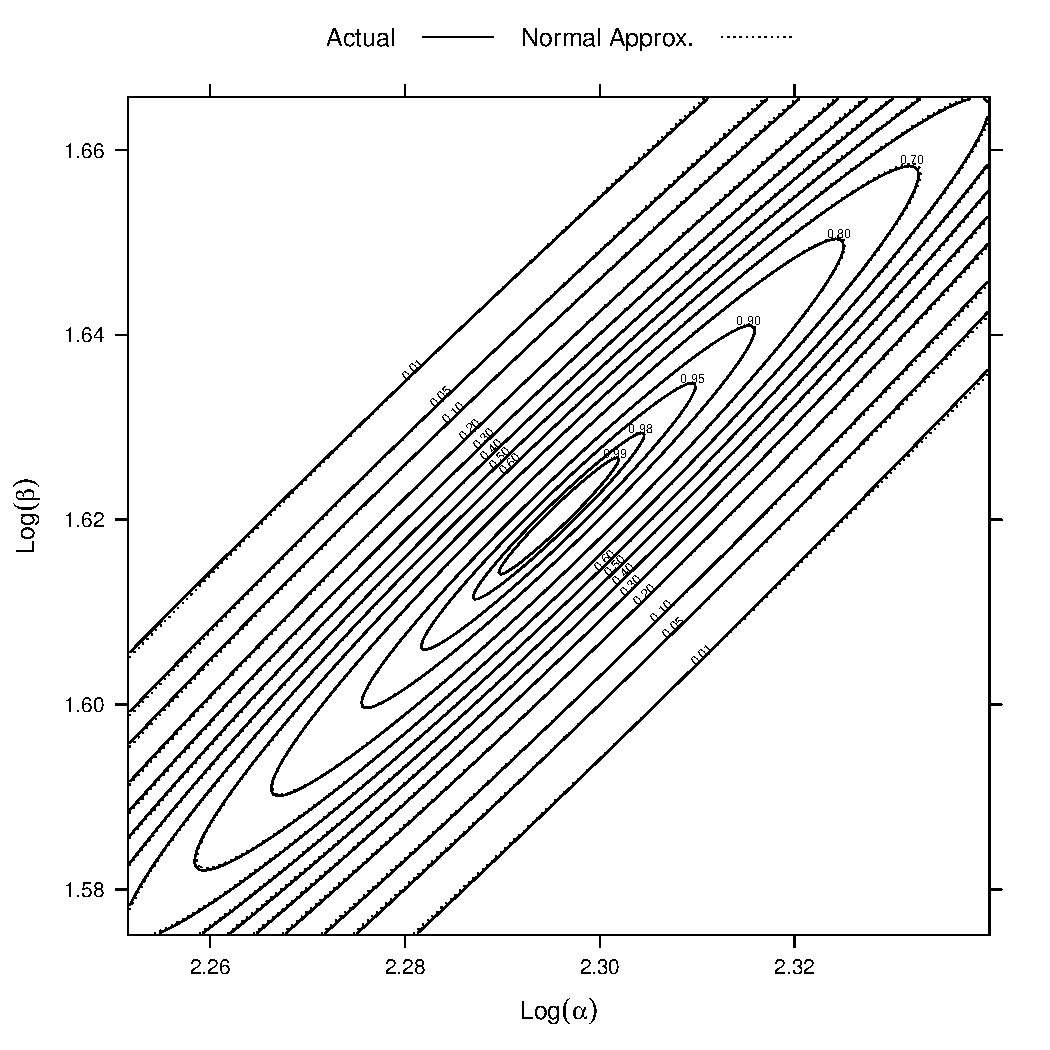
\includegraphics[width=\textwidth]{figures/proteomics/gamma_normal_approx}

\caption{Normal approximation to the conditional posterior of $(\log \alpha_\sigma, \log \beta_\sigma)$. Contours of the log-conditional posterior and proposal for $\alpha_\sigma=10$ and $\beta_\sigma=5$ with $n=1000$ observations.\label{fig:Normal-approximation-to-log-gamma-pars}} 
\end{figure}




\subsection{Updates for censoring model parameters}


\subsubsection{Gibbs update for $\pi^{rnd}$}

The conditional posterior distribution of the random censoring probability is straightforward and conjugate, enabling a direct update:
\begin{equation*}
\pi^{rnd} | \bm M, \bm \Theta_{-\pi^{rnd}} \sim Beta\left( \sum_{ikl} R_{ikl}, \sum_{ikl} (1 - R_{ikl}) \right) .
\end{equation*}


\subsubsection{Metropolis-Hastings update for intensity-based censoring parameters}

The parameters of the intensity-based censoring model, $\bm \eta$,
are updated using an independence chain Metropolis-Hastings sampler.
%
We first obtain the mode of the conditional posterior of $\bm \eta$, $\hat{\bm \eta}$, using standard GLM estimation techniques (Fisher scoring).
This estimation naturally yields the expected negative Hessian of this conditional posterior $\mathcal{I}(\hat{\bm{\eta}})$.
We then draw proposal as
\begin{equation*}
\bm{\eta}^* = \hat{\bm{\eta}} + \sqrt{\frac{\nu}{\nu - 2}} \mathcal{I}(\hat{\bm{\eta}})^{-1/2} \bm{t}_\nu,
\end{equation*}
where $\bm{t}_\nu$ is defined as before.


\subsection{Metropolis-Hastings update for number of states parameters $(r, \lambda)$}
\label{sec:draw_number_of_states_hyperparameters}

The conditional posterior distribution of $(r, \lambda)$ is not of conjugate form regardless of the prior distribution.
For our inference, we take $r \sim LogNormal(\mu_{0r}, \sigma^2_{0r})$ independent of $\lambda \sim Beta(\alpha_{0\lambda}, \beta_{0\lambda})$ a priori.
We construct a proposal for these parameters by first transforming them to $(\log r, \logit \lambda)$.
We then estimate a normal approximation to the joint conditional posterior of these transformed parameters.

As in Section \ref{sec:var_hyperparam_updates}, we can analytically maximize  the conditional posterior over one parameter given the other.
Maximizing over $\log r$ yields
%
\begin{equation*}
\widehat{\logit \lambda} = \frac{\sum_{ik}r + \alpha_{0r}}{\sum_{ik}r+\sum_{ik}(s_{ik}-1) + \alpha_{0r} + \beta_{0r}} .
\end{equation*}
%
This reduces estimation of the conditional posterior mode to univariate optimization over $\logit r$.
Following this optimization, we compute the negative Hessian of the log-conditional posteriors $\hat{\mathcal{I}}(\widehat{\log r}, \widehat{\logit \lambda})$ and propose as
\begin{equation*}
(\log r^*, \logit \lambda^*) \mid \bm s \sim \left(\begin{array}{c}
\widehat{\log r} \\
\widehat{\logit \lambda}
\end{array}\right) +
\sqrt{\frac{\nu}{\nu - 2}} \hat{\mathcal{I}}(\widehat{\log r}, \widehat{\logit \lambda})^{-1/2} \bm{t_{\nu}} .
\end{equation*}


\begin{figure}
\centering
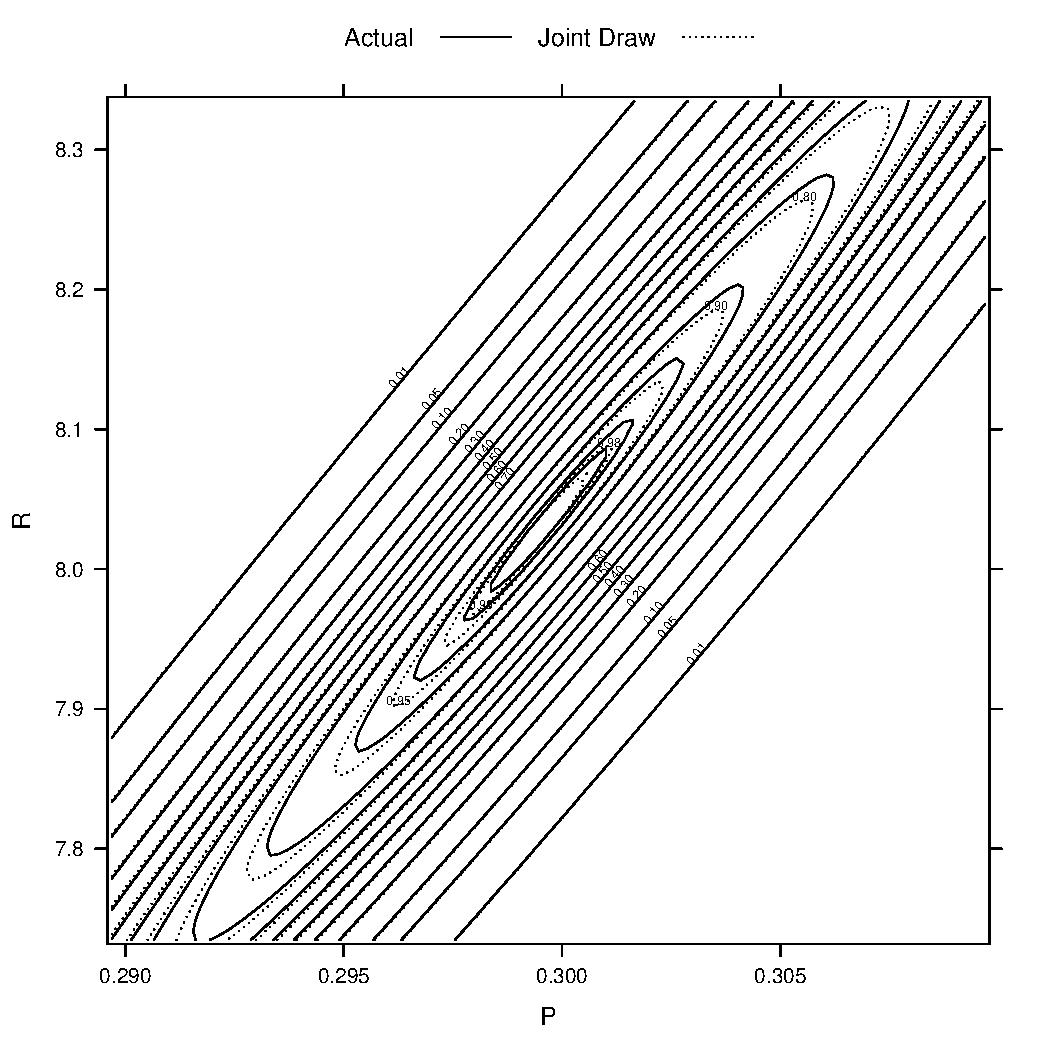
\includegraphics[width=1\textwidth]{figures/proteomics/Neg_Bin_Parameter_Draw}
\caption{Conditional posterior contours for $(r, \lambda)$.\label{fig:Negative-binomial-parameters}}
\end{figure}


 %%% %%% %%%
 %%% %%% %%%
 %%% %%% %%%

\clearpage

\section{Additional simulation results}

\begin{sidewaystable}
\begin{center}
\caption{Simulation analysis of protein abundance estimates by $\zeta_i$ and $m_i$, 90m gradient. All estimates are $\pm$ one standard deviation. \label{tab:sim_estimates_90m}}
\begin{tabular}{ccc|c|ccccc}
 Grad. & $\zeta_i$ & $m_i$ & Posterior Mean & Sum Int. & Mean Int. & Med. Int. & AMI & emPAI \\ 
  \hline
90m &   3 &  20 & $3.30 \pm 0.33$ & $2.33 \pm 0.92$ & $3.78 \pm 0.87$ & $4.85 \pm 0.77$ & $3.87 \pm 0.84$ & $5.98 \pm 0.16$ \\ 
  90m &   3 &  30 & $3.19 \pm 0.33$ & $2.38 \pm 0.78$ & $3.79 \pm 0.73$ & $4.84 \pm 0.67$ & $3.89 \pm 0.72$ & $5.84 \pm 0.19$ \\ 
  90m &   3 &  40 & $3.09 \pm 0.35$ & $2.46 \pm 0.81$ & $3.84 \pm 0.73$ & $4.89 \pm 0.64$ & $3.94 \pm 0.72$ & $5.75 \pm 0.20$ \\ 
  90m &   3 &  50 & $3.03 \pm 0.34$ & $2.40 \pm 0.76$ & $3.73 \pm 0.66$ & $4.76 \pm 0.62$ & $3.83 \pm 0.65$ & $5.68 \pm 0.21$ \\ 
  90m &   3 &  60 & $2.99 \pm 0.38$ & $2.56 \pm 0.85$ & $3.86 \pm 0.75$ & $4.86 \pm 0.64$ & $3.95 \pm 0.74$ & $5.64 \pm 0.24$ \\ 
   \hline
90m &   4 &  20 & $3.91 \pm 0.38$ & $3.23 \pm 0.68$ & $4.37 \pm 0.60$ & $5.29 \pm 0.52$ & $4.46 \pm 0.59$ & $6.32 \pm 0.24$ \\ 
  90m &   4 &  30 & $3.87 \pm 0.39$ & $3.36 \pm 0.65$ & $4.37 \pm 0.53$ & $5.22 \pm 0.45$ & $4.45 \pm 0.52$ & $6.28 \pm 0.26$ \\ 
  90m &   4 &  40 & $3.87 \pm 0.38$ & $3.57 \pm 0.64$ & $4.46 \pm 0.53$ & $5.26 \pm 0.40$ & $4.54 \pm 0.51$ & $6.27 \pm 0.26$ \\ 
  90m &   4 &  50 & $3.87 \pm 0.38$ & $3.64 \pm 0.58$ & $4.45 \pm 0.49$ & $5.26 \pm 0.37$ & $4.53 \pm 0.47$ & $6.25 \pm 0.25$ \\ 
  90m &   4 &  60 & $3.87 \pm 0.33$ & $3.76 \pm 0.55$ & $4.48 \pm 0.46$ & $5.24 \pm 0.33$ & $4.56 \pm 0.45$ & $6.26 \pm 0.22$ \\ 
   \hline
90m &   5 &  20 & $4.92 \pm 0.33$ & $4.34 \pm 0.52$ & $5.02 \pm 0.48$ & $5.67 \pm 0.29$ & $5.07 \pm 0.47$ & $6.92 \pm 0.20$ \\ 
  90m &   5 &  30 & $4.95 \pm 0.28$ & $4.61 \pm 0.49$ & $5.10 \pm 0.46$ & $5.69 \pm 0.27$ & $5.16 \pm 0.45$ & $6.93 \pm 0.16$ \\ 
  90m &   5 &  40 & $4.96 \pm 0.22$ & $4.81 \pm 0.50$ & $5.17 \pm 0.48$ & $5.68 \pm 0.23$ & $5.22 \pm 0.47$ & $6.94 \pm 0.13$ \\ 
  90m &   5 &  50 & $4.97 \pm 0.20$ & $4.89 \pm 0.44$ & $5.16 \pm 0.42$ & $5.69 \pm 0.22$ & $5.21 \pm 0.42$ & $6.94 \pm 0.12$ \\ 
  90m &   5 &  60 & $4.98 \pm 0.21$ & $4.97 \pm 0.43$ & $5.16 \pm 0.41$ & $5.66 \pm 0.19$ & $5.21 \pm 0.41$ & $6.94 \pm 0.12$ \\ 
   \hline
90m &   6 &  20 & $5.95 \pm 0.28$ & $5.48 \pm 0.50$ & $5.89 \pm 0.49$ & $6.24 \pm 0.26$ & $5.91 \pm 0.48$ & $7.36 \pm 0.14$ \\ 
  90m &   6 &  30 & $5.94 \pm 0.21$ & $5.66 \pm 0.45$ & $5.89 \pm 0.46$ & $6.23 \pm 0.23$ & $5.91 \pm 0.46$ & $7.36 \pm 0.11$ \\ 
  90m &   6 &  40 & $5.97 \pm 0.21$ & $5.83 \pm 0.45$ & $5.94 \pm 0.45$ & $6.25 \pm 0.21$ & $5.96 \pm 0.45$ & $7.36 \pm 0.10$ \\ 
  90m &   6 &  50 & $5.97 \pm 0.16$ & $5.96 \pm 0.45$ & $5.96 \pm 0.46$ & $6.25 \pm 0.18$ & $5.98 \pm 0.46$ & $7.36 \pm 0.09$ \\ 
  90m &   6 &  60 & $5.99 \pm 0.16$ & $6.04 \pm 0.42$ & $5.96 \pm 0.43$ & $6.25 \pm 0.18$ & $5.98 \pm 0.43$ & $7.37 \pm 0.08$ \\ 
   \hline
90m &   7 &  20 & $6.94 \pm 0.24$ & $6.45 \pm 0.47$ & $6.76 \pm 0.47$ & $7.03 \pm 0.25$ & $6.77 \pm 0.46$ & $7.54 \pm 0.10$ \\ 
  90m &   7 &  30 & $6.94 \pm 0.21$ & $6.65 \pm 0.43$ & $6.78 \pm 0.43$ & $7.01 \pm 0.22$ & $6.79 \pm 0.43$ & $7.56 \pm 0.09$ \\ 
  90m &   7 &  40 & $6.92 \pm 0.17$ & $6.79 \pm 0.43$ & $6.81 \pm 0.43$ & $6.99 \pm 0.19$ & $6.81 \pm 0.43$ & $7.55 \pm 0.08$ \\ 
  90m &   7 &  50 & $6.94 \pm 0.16$ & $6.96 \pm 0.46$ & $6.88 \pm 0.46$ & $7.00 \pm 0.18$ & $6.88 \pm 0.46$ & $7.55 \pm 0.07$ \\ 
  90m &   7 &  60 & $6.94 \pm 0.15$ & $7.03 \pm 0.42$ & $6.87 \pm 0.42$ & $7.01 \pm 0.16$ & $6.87 \pm 0.42$ & $7.55 \pm 0.07$ \\ 
   \hline
90m &   8 &  20 & $7.94 \pm 0.21$ & $7.46 \pm 0.45$ & $7.75 \pm 0.42$ & $7.95 \pm 0.24$ & $7.75 \pm 0.42$ & $7.59 \pm 0.09$ \\ 
  90m &   8 &  30 & $7.93 \pm 0.18$ & $7.69 \pm 0.40$ & $7.81 \pm 0.39$ & $7.93 \pm 0.21$ & $7.81 \pm 0.39$ & $7.59 \pm 0.08$ \\ 
  90m &   8 &  40 & $7.94 \pm 0.15$ & $7.83 \pm 0.40$ & $7.82 \pm 0.39$ & $7.94 \pm 0.17$ & $7.82 \pm 0.39$ & $7.60 \pm 0.07$ \\ 
  90m &   8 &  50 & $7.95 \pm 0.14$ & $7.94 \pm 0.38$ & $7.83 \pm 0.39$ & $7.96 \pm 0.17$ & $7.83 \pm 0.39$ & $7.60 \pm 0.06$ \\ 
  90m &   8 &  60 & $7.95 \pm 0.13$ & $8.01 \pm 0.34$ & $7.82 \pm 0.36$ & $7.96 \pm 0.15$ & $7.83 \pm 0.36$ & $7.60 \pm 0.06$ \\ 
   \hline
\end{tabular}
\end{center}
\end{sidewaystable}


\begin{sidewaystable}
\begin{center}
\caption{Simulation analysis of protein abundance estimates by $\zeta_i$ and $m_i$, 180m gradient. All estimates are $\pm$ one standard deviation. \label{tab:sim_estimates_180m}}
\begin{tabular}{ccc|c|ccccc}
 Grad. & $\zeta_i$ & $m_i$ & Posterior Mean & Sum Int. & Mean Int. & Med. Int. & AMI & emPAI \\ 
 \hline
180m &   3 &  20 & $3.13 \pm 0.42$ & $2.08 \pm 0.85$ & $3.46 \pm 0.80$ & $4.75 \pm 0.70$ & $3.59 \pm 0.79$ & $6.02 \pm 0.21$ \\ 
  180m &   3 &  30 & $2.97 \pm 0.44$ & $2.13 \pm 0.89$ & $3.47 \pm 0.80$ & $4.74 \pm 0.68$ & $3.60 \pm 0.79$ & $5.88 \pm 0.23$ \\ 
  180m &   3 &  40 & $2.93 \pm 0.43$ & $2.30 \pm 0.87$ & $3.56 \pm 0.76$ & $4.77 \pm 0.64$ & $3.69 \pm 0.76$ & $5.83 \pm 0.25$ \\ 
  180m &   3 &  50 & $2.91 \pm 0.44$ & $2.35 \pm 0.86$ & $3.57 \pm 0.73$ & $4.77 \pm 0.60$ & $3.69 \pm 0.72$ & $5.78 \pm 0.28$ \\ 
  180m &   3 &  60 & $2.90 \pm 0.45$ & $2.45 \pm 0.86$ & $3.59 \pm 0.72$ & $4.77 \pm 0.58$ & $3.72 \pm 0.72$ & $5.77 \pm 0.28$ \\ 
   \hline
180m &   4 &  20 & $3.89 \pm 0.47$ & $3.13 \pm 0.77$ & $4.15 \pm 0.67$ & $5.22 \pm 0.49$ & $4.26 \pm 0.66$ & $6.44 \pm 0.29$ \\ 
  180m &   4 &  30 & $3.89 \pm 0.39$ & $3.35 \pm 0.70$ & $4.20 \pm 0.62$ & $5.15 \pm 0.42$ & $4.30 \pm 0.61$ & $6.44 \pm 0.25$ \\ 
  180m &   4 &  40 & $3.91 \pm 0.36$ & $3.59 \pm 0.74$ & $4.30 \pm 0.66$ & $5.17 \pm 0.38$ & $4.41 \pm 0.65$ & $6.44 \pm 0.22$ \\ 
  180m &   4 &  50 & $3.93 \pm 0.33$ & $3.65 \pm 0.64$ & $4.26 \pm 0.57$ & $5.18 \pm 0.32$ & $4.37 \pm 0.57$ & $6.44 \pm 0.20$ \\ 
  180m &   4 &  60 & $3.93 \pm 0.33$ & $3.77 \pm 0.62$ & $4.30 \pm 0.55$ & $5.17 \pm 0.33$ & $4.41 \pm 0.54$ & $6.44 \pm 0.20$ \\ 
   \hline
180m &   5 &  20 & $4.95 \pm 0.33$ & $4.27 \pm 0.58$ & $4.87 \pm 0.55$ & $5.63 \pm 0.29$ & $4.93 \pm 0.54$ & $7.01 \pm 0.20$ \\ 
  180m &   5 &  30 & $4.97 \pm 0.28$ & $4.59 \pm 0.61$ & $5.01 \pm 0.60$ & $5.68 \pm 0.27$ & $5.07 \pm 0.59$ & $7.01 \pm 0.15$ \\ 
  180m &   5 &  40 & $4.98 \pm 0.22$ & $4.70 \pm 0.55$ & $4.98 \pm 0.55$ & $5.64 \pm 0.24$ & $5.05 \pm 0.54$ & $7.02 \pm 0.12$ \\ 
  180m &   5 &  50 & $4.99 \pm 0.19$ & $4.86 \pm 0.57$ & $5.04 \pm 0.57$ & $5.65 \pm 0.23$ & $5.11 \pm 0.57$ & $7.03 \pm 0.11$ \\ 
  180m &   5 &  60 & $5.01 \pm 0.20$ & $4.89 \pm 0.53$ & $5.00 \pm 0.53$ & $5.65 \pm 0.23$ & $5.07 \pm 0.52$ & $7.01 \pm 0.10$ \\ 
   \hline
180m &   6 &  20 & $5.96 \pm 0.28$ & $5.35 \pm 0.58$ & $5.74 \pm 0.58$ & $6.23 \pm 0.28$ & $5.77 \pm 0.57$ & $7.37 \pm 0.14$ \\ 
  180m &   6 &  30 & $5.98 \pm 0.22$ & $5.61 \pm 0.56$ & $5.81 \pm 0.57$ & $6.24 \pm 0.25$ & $5.84 \pm 0.56$ & $7.39 \pm 0.11$ \\ 
  180m &   6 &  40 & $5.96 \pm 0.18$ & $5.68 \pm 0.50$ & $5.75 \pm 0.50$ & $6.21 \pm 0.20$ & $5.78 \pm 0.50$ & $7.39 \pm 0.09$ \\ 
  180m &   6 &  50 & $5.99 \pm 0.18$ & $5.84 \pm 0.50$ & $5.82 \pm 0.50$ & $6.23 \pm 0.19$ & $5.85 \pm 0.50$ & $7.38 \pm 0.09$ \\ 
  180m &   6 &  60 & $5.99 \pm 0.16$ & $5.90 \pm 0.51$ & $5.80 \pm 0.52$ & $6.22 \pm 0.17$ & $5.83 \pm 0.52$ & $7.38 \pm 0.08$ \\ 
   \hline
180m &   7 &  20 & $6.96 \pm 0.23$ & $6.36 \pm 0.54$ & $6.68 \pm 0.55$ & $7.02 \pm 0.26$ & $6.69 \pm 0.55$ & $7.53 \pm 0.11$ \\ 
  180m &   7 &  30 & $6.94 \pm 0.21$ & $6.61 \pm 0.57$ & $6.75 \pm 0.58$ & $7.03 \pm 0.23$ & $6.76 \pm 0.58$ & $7.53 \pm 0.08$ \\ 
  180m &   7 &  40 & $6.94 \pm 0.17$ & $6.70 \pm 0.52$ & $6.71 \pm 0.54$ & $7.01 \pm 0.20$ & $6.72 \pm 0.54$ & $7.53 \pm 0.07$ \\ 
  180m &   7 &  50 & $6.94 \pm 0.16$ & $6.84 \pm 0.54$ & $6.75 \pm 0.55$ & $7.01 \pm 0.18$ & $6.75 \pm 0.55$ & $7.53 \pm 0.07$ \\ 
  180m &   7 &  60 & $6.95 \pm 0.15$ & $6.95 \pm 0.52$ & $6.78 \pm 0.54$ & $7.02 \pm 0.17$ & $6.79 \pm 0.54$ & $7.53 \pm 0.06$ \\ 
   \hline
180m &   8 &  20 & $7.91 \pm 0.21$ & $7.33 \pm 0.56$ & $7.63 \pm 0.54$ & $7.92 \pm 0.25$ & $7.63 \pm 0.54$ & $7.57 \pm 0.09$ \\ 
  180m &   8 &  30 & $7.94 \pm 0.18$ & $7.57 \pm 0.54$ & $7.69 \pm 0.53$ & $7.95 \pm 0.20$ & $7.69 \pm 0.52$ & $7.58 \pm 0.07$ \\ 
  180m &   8 &  40 & $7.94 \pm 0.14$ & $7.74 \pm 0.46$ & $7.73 \pm 0.47$ & $7.95 \pm 0.18$ & $7.73 \pm 0.47$ & $7.57 \pm 0.07$ \\ 
  180m &   8 &  50 & $7.94 \pm 0.14$ & $7.86 \pm 0.48$ & $7.76 \pm 0.50$ & $7.95 \pm 0.16$ & $7.75 \pm 0.50$ & $7.57 \pm 0.06$ \\ 
  180m &   8 &  60 & $7.94 \pm 0.13$ & $7.94 \pm 0.43$ & $7.75 \pm 0.46$ & $7.94 \pm 0.16$ & $7.75 \pm 0.46$ & $7.57 \pm 0.05$ \\ 
   \hline
\end{tabular}
\end{center}
\end{sidewaystable}


\begin{sidewaystable}
\begin{center}
\caption{Simulation analysis of protein abundance estimates by $\zeta_i$ and $m_i$, 360m gradient. All estimates are $\pm$ one standard deviation. \label{tab:sim_estimates_360m}}
\begin{tabular}{ccc|c|ccccc}
 Grad. & $\zeta_i$ & $m_i$ & Posterior Mean & Sum Int. & Mean Int. & Med. Int. & AMI & emPAI \\ 
 \hline
360m &   3 &  20 & $3.07 \pm 0.34$ & $2.25 \pm 0.67$ & $3.59 \pm 0.58$ & $4.63 \pm 0.52$ & $3.78 \pm 0.57$ & $6.02 \pm 0.24$ \\ 
  360m &   3 &  30 & $3.00 \pm 0.37$ & $2.32 \pm 0.70$ & $3.57 \pm 0.57$ & $4.57 \pm 0.44$ & $3.76 \pm 0.54$ & $5.91 \pm 0.27$ \\ 
  360m &   3 &  40 & $2.94 \pm 0.37$ & $2.45 \pm 0.67$ & $3.65 \pm 0.54$ & $4.64 \pm 0.41$ & $3.84 \pm 0.52$ & $5.84 \pm 0.28$ \\ 
  360m &   3 &  50 & $2.97 \pm 0.36$ & $2.55 \pm 0.68$ & $3.65 \pm 0.52$ & $4.61 \pm 0.41$ & $3.84 \pm 0.51$ & $5.83 \pm 0.28$ \\ 
  360m &   3 &  60 & $2.97 \pm 0.38$ & $2.65 \pm 0.67$ & $3.69 \pm 0.51$ & $4.62 \pm 0.37$ & $3.87 \pm 0.49$ & $5.83 \pm 0.30$ \\ 
   \hline
360m &   4 &  20 & $3.97 \pm 0.33$ & $3.36 \pm 0.52$ & $4.17 \pm 0.45$ & $4.95 \pm 0.30$ & $4.30 \pm 0.43$ & $6.64 \pm 0.24$ \\ 
  360m &   4 &  30 & $3.96 \pm 0.28$ & $3.59 \pm 0.47$ & $4.23 \pm 0.42$ & $4.92 \pm 0.25$ & $4.36 \pm 0.40$ & $6.63 \pm 0.20$ \\ 
  360m &   4 &  40 & $4.01 \pm 0.25$ & $3.80 \pm 0.49$ & $4.29 \pm 0.45$ & $4.95 \pm 0.23$ & $4.41 \pm 0.44$ & $6.67 \pm 0.18$ \\ 
  360m &   4 &  50 & $3.98 \pm 0.21$ & $3.85 \pm 0.45$ & $4.26 \pm 0.41$ & $4.92 \pm 0.20$ & $4.39 \pm 0.40$ & $6.64 \pm 0.15$ \\ 
  360m &   4 &  60 & $4.03 \pm 0.20$ & $3.94 \pm 0.43$ & $4.26 \pm 0.39$ & $4.92 \pm 0.21$ & $4.39 \pm 0.37$ & $6.66 \pm 0.14$ \\ 
   \hline
360m &   5 &  20 & $4.99 \pm 0.24$ & $4.46 \pm 0.42$ & $4.90 \pm 0.41$ & $5.35 \pm 0.22$ & $4.96 \pm 0.41$ & $7.21 \pm 0.15$ \\ 
  360m &   5 &  30 & $4.99 \pm 0.20$ & $4.66 \pm 0.41$ & $4.93 \pm 0.40$ & $5.36 \pm 0.20$ & $4.99 \pm 0.40$ & $7.20 \pm 0.12$ \\ 
  360m &   5 &  40 & $5.00 \pm 0.17$ & $4.85 \pm 0.41$ & $4.99 \pm 0.41$ & $5.36 \pm 0.18$ & $5.04 \pm 0.40$ & $7.21 \pm 0.10$ \\ 
  360m &   5 &  50 & $5.00 \pm 0.16$ & $4.94 \pm 0.41$ & $4.98 \pm 0.41$ & $5.35 \pm 0.16$ & $5.04 \pm 0.40$ & $7.21 \pm 0.10$ \\ 
  360m &   5 &  60 & $5.05 \pm 0.14$ & $5.05 \pm 0.39$ & $5.01 \pm 0.39$ & $5.37 \pm 0.16$ & $5.07 \pm 0.38$ & $7.21 \pm 0.08$ \\ 
   \hline
360m &   6 &  20 & $5.98 \pm 0.22$ & $5.52 \pm 0.47$ & $5.85 \pm 0.47$ & $6.07 \pm 0.24$ & $5.86 \pm 0.46$ & $7.44 \pm 0.11$ \\ 
  360m &   6 &  30 & $5.96 \pm 0.19$ & $5.71 \pm 0.44$ & $5.86 \pm 0.44$ & $6.06 \pm 0.20$ & $5.87 \pm 0.43$ & $7.43 \pm 0.10$ \\ 
  360m &   6 &  40 & $5.96 \pm 0.17$ & $5.81 \pm 0.39$ & $5.84 \pm 0.38$ & $6.06 \pm 0.16$ & $5.85 \pm 0.38$ & $7.43 \pm 0.08$ \\ 
  360m &   6 &  50 & $5.95 \pm 0.15$ & $5.94 \pm 0.40$ & $5.87 \pm 0.40$ & $6.04 \pm 0.16$ & $5.89 \pm 0.40$ & $7.43 \pm 0.07$ \\ 
  360m &   6 &  60 & $5.97 \pm 0.15$ & $6.05 \pm 0.41$ & $5.90 \pm 0.42$ & $6.05 \pm 0.16$ & $5.91 \pm 0.41$ & $7.43 \pm 0.07$ \\ 
   \hline
360m &   7 &  20 & $6.95 \pm 0.22$ & $6.52 \pm 0.44$ & $6.82 \pm 0.43$ & $6.98 \pm 0.26$ & $6.82 \pm 0.43$ & $7.48 \pm 0.10$ \\ 
  360m &   7 &  30 & $6.96 \pm 0.16$ & $6.72 \pm 0.44$ & $6.85 \pm 0.43$ & $6.99 \pm 0.19$ & $6.86 \pm 0.43$ & $7.48 \pm 0.08$ \\ 
  360m &   7 &  40 & $6.94 \pm 0.15$ & $6.85 \pm 0.38$ & $6.85 \pm 0.38$ & $6.96 \pm 0.19$ & $6.85 \pm 0.38$ & $7.48 \pm 0.07$ \\ 
  360m &   7 &  50 & $6.95 \pm 0.13$ & $6.97 \pm 0.41$ & $6.88 \pm 0.41$ & $6.97 \pm 0.16$ & $6.89 \pm 0.41$ & $7.48 \pm 0.07$ \\ 
  360m &   7 &  60 & $6.96 \pm 0.12$ & $7.06 \pm 0.41$ & $6.89 \pm 0.41$ & $6.98 \pm 0.14$ & $6.89 \pm 0.41$ & $7.48 \pm 0.06$ \\ 
   \hline
360m &   8 &  20 & $7.94 \pm 0.17$ & $7.45 \pm 0.42$ & $7.75 \pm 0.39$ & $7.96 \pm 0.21$ & $7.76 \pm 0.38$ & $7.49 \pm 0.09$ \\ 
  360m &   8 &  30 & $7.96 \pm 0.15$ & $7.71 \pm 0.38$ & $7.83 \pm 0.37$ & $7.97 \pm 0.19$ & $7.84 \pm 0.36$ & $7.48 \pm 0.08$ \\ 
  360m &   8 &  40 & $7.96 \pm 0.13$ & $7.88 \pm 0.36$ & $7.88 \pm 0.35$ & $7.96 \pm 0.16$ & $7.88 \pm 0.35$ & $7.48 \pm 0.07$ \\ 
  360m &   8 &  50 & $7.97 \pm 0.13$ & $7.96 \pm 0.34$ & $7.86 \pm 0.35$ & $7.97 \pm 0.14$ & $7.86 \pm 0.34$ & $7.49 \pm 0.06$ \\ 
  360m &   8 &  60 & $7.96 \pm 0.12$ & $8.05 \pm 0.33$ & $7.87 \pm 0.34$ & $7.97 \pm 0.14$ & $7.88 \pm 0.34$ & $7.48 \pm 0.06$ \\ 
   \hline
\end{tabular}
\end{center}
\end{sidewaystable}

% Coverage results

% latex table generated in R 2.12.2 by xtable 1.5-6 package
% Tue Apr  2 15:10:13 2013
\begin{table}
\begin{center}
\caption{Coverage of HPD posterior intervals for $\zeta_i$ in simulation study, 90m gradient
\label{tab:sim_coverage_90m}}
\begin{tabular}{ccc|cccc}
 Grad. & $\zeta_i$ & $m_i$ & 68\% & 90\% & 95\% & 99\% \\ 
  \hline
90m &   3 &  20 & 0.69 & 0.94 & 0.97 & 0.98 \\ 
  90m &   3 &  30 & 0.71 & 0.92 & 0.95 & 0.99 \\ 
  90m &   3 &  40 & 0.75 & 0.92 & 0.96 & 0.99 \\ 
  90m &   3 &  50 & 0.79 & 0.93 & 0.95 & 0.98 \\ 
  90m &   3 &  60 & 0.75 & 0.94 & 0.97 & 0.99 \\ 
   \hline
90m &   4 &  20 & 0.74 & 0.95 & 0.97 & 0.99 \\ 
  90m &   4 &  30 & 0.70 & 0.92 & 0.96 & 0.98 \\ 
  90m &   4 &  40 & 0.67 & 0.88 & 0.93 & 0.98 \\ 
  90m &   4 &  50 & 0.63 & 0.88 & 0.93 & 0.97 \\ 
  90m &   4 &  60 & 0.70 & 0.91 & 0.95 & 0.97 \\ 
   \hline
90m &   5 &  20 & 0.67 & 0.88 & 0.94 & 0.99 \\ 
  90m &   5 &  30 & 0.63 & 0.86 & 0.92 & 0.99 \\ 
  90m &   5 &  40 & 0.71 & 0.93 & 0.96 & 1.00 \\ 
  90m &   5 &  50 & 0.71 & 0.90 & 0.97 & 0.99 \\ 
  90m &   5 &  60 & 0.64 & 0.85 & 0.91 & 0.98 \\ 
   \hline
90m &   6 &  20 & 0.63 & 0.86 & 0.93 & 0.99 \\ 
  90m &   6 &  30 & 0.65 & 0.89 & 0.94 & 0.98 \\ 
  90m &   6 &  40 & 0.65 & 0.86 & 0.92 & 0.98 \\ 
  90m &   6 &  50 & 0.67 & 0.90 & 0.96 & 0.99 \\ 
  90m &   6 &  60 & 0.67 & 0.91 & 0.95 & 0.98 \\ 
   \hline
90m &   7 &  20 & 0.66 & 0.90 & 0.94 & 0.99 \\ 
  90m &   7 &  30 & 0.63 & 0.86 & 0.90 & 0.98 \\ 
  90m &   7 &  40 & 0.61 & 0.85 & 0.93 & 0.98 \\ 
  90m &   7 &  50 & 0.65 & 0.88 & 0.94 & 0.99 \\ 
  90m &   7 &  60 & 0.65 & 0.87 & 0.93 & 0.97 \\ 
   \hline
90m &   8 &  20 & 0.65 & 0.88 & 0.93 & 0.99 \\ 
  90m &   8 &  30 & 0.63 & 0.88 & 0.93 & 0.99 \\ 
  90m &   8 &  40 & 0.65 & 0.89 & 0.94 & 0.98 \\ 
  90m &   8 &  50 & 0.65 & 0.89 & 0.92 & 0.98 \\ 
  90m &   8 &  60 & 0.64 & 0.87 & 0.92 & 0.98 \\ 
   \hline
\end{tabular}
\end{center}
\end{table}

\begin{table}
\begin{center}
\caption{Coverage of HPD posterior intervals for $\zeta_i$ in simulation study, 180m gradient
\label{tab:sim_coverage_180m}}
\begin{tabular}{ccc|cccc}
 Grad. & $\zeta_i$ & $m_i$ & 68\% & 90\% & 95\% & 99\% \\ 
  \hline
180m &   3 &  20 & 0.71 & 0.91 & 0.97 & 0.99 \\ 
  180m &   3 &  30 & 0.78 & 0.91 & 0.96 & 0.99 \\ 
  180m &   3 &  40 & 0.77 & 0.93 & 0.97 & 0.99 \\ 
  180m &   3 &  50 & 0.72 & 0.92 & 0.96 & 0.99 \\ 
  180m &   3 &  60 & 0.66 & 0.90 & 0.93 & 0.98 \\ 
   \hline
180m &   4 &  20 & 0.66 & 0.89 & 0.95 & 0.99 \\ 
  180m &   4 &  30 & 0.66 & 0.89 & 0.95 & 0.98 \\ 
  180m &   4 &  40 & 0.68 & 0.88 & 0.93 & 0.97 \\ 
  180m &   4 &  50 & 0.63 & 0.87 & 0.93 & 0.97 \\ 
  180m &   4 &  60 & 0.59 & 0.86 & 0.91 & 0.97 \\ 
   \hline
180m &   5 &  20 & 0.67 & 0.87 & 0.93 & 0.97 \\ 
  180m &   5 &  30 & 0.68 & 0.90 & 0.94 & 0.98 \\ 
  180m &   5 &  40 & 0.69 & 0.90 & 0.95 & 0.99 \\ 
  180m &   5 &  50 & 0.69 & 0.90 & 0.94 & 0.99 \\ 
  180m &   5 &  60 & 0.66 & 0.87 & 0.94 & 0.98 \\ 
   \hline
180m &   6 &  20 & 0.65 & 0.88 & 0.94 & 0.98 \\ 
  180m &   6 &  30 & 0.65 & 0.92 & 0.95 & 1.00 \\ 
  180m &   6 &  40 & 0.71 & 0.88 & 0.94 & 0.99 \\ 
  180m &   6 &  50 & 0.68 & 0.86 & 0.94 & 0.98 \\ 
  180m &   6 &  60 & 0.71 & 0.89 & 0.93 & 1.00 \\ 
   \hline
180m &   7 &  20 & 0.68 & 0.91 & 0.97 & 0.99 \\ 
  180m &   7 &  30 & 0.69 & 0.88 & 0.94 & 0.97 \\ 
  180m &   7 &  40 & 0.64 & 0.87 & 0.93 & 0.98 \\ 
  180m &   7 &  50 & 0.65 & 0.87 & 0.92 & 0.97 \\ 
  180m &   7 &  60 & 0.66 & 0.88 & 0.93 & 0.98 \\ 
   \hline
180m &   8 &  20 & 0.65 & 0.88 & 0.94 & 0.99 \\ 
  180m &   8 &  30 & 0.62 & 0.87 & 0.93 & 0.98 \\ 
  180m &   8 &  40 & 0.68 & 0.90 & 0.94 & 0.98 \\ 
  180m &   8 &  50 & 0.68 & 0.87 & 0.93 & 0.97 \\ 
  180m &   8 &  60 & 0.60 & 0.86 & 0.94 & 0.98 \\ 
   \hline
\end{tabular}
\end{center}
\end{table}

\begin{table}
\begin{center}
\caption{Coverage of HPD posterior intervals for $\zeta_i$ in simulation study, 360m gradient
\label{tab:sim_coverage_360m}}
\begin{tabular}{ccc|cccc}
 Grad. & $\zeta_i$ & $m_i$ & 68\% & 90\% & 95\% & 99\% \\ 
 \hline
360m &   3 &  20 & 0.75 & 0.91 & 0.95 & 0.99 \\ 
  360m &   3 &  30 & 0.73 & 0.90 & 0.93 & 0.98 \\ 
  360m &   3 &  40 & 0.72 & 0.93 & 0.97 & 0.99 \\ 
  360m &   3 &  50 & 0.68 & 0.89 & 0.94 & 0.98 \\ 
  360m &   3 &  60 & 0.64 & 0.85 & 0.91 & 0.97 \\ 
   \hline
360m &   4 &  20 & 0.64 & 0.88 & 0.93 & 0.98 \\ 
  360m &   4 &  30 & 0.62 & 0.88 & 0.94 & 0.99 \\ 
  360m &   4 &  40 & 0.62 & 0.85 & 0.91 & 0.97 \\ 
  360m &   4 &  50 & 0.67 & 0.88 & 0.94 & 0.99 \\ 
  360m &   4 &  60 & 0.60 & 0.87 & 0.93 & 0.98 \\ 
   \hline
360m &   5 &  20 & 0.70 & 0.89 & 0.95 & 0.99 \\ 
  360m &   5 &  30 & 0.69 & 0.91 & 0.94 & 0.99 \\ 
  360m &   5 &  40 & 0.68 & 0.90 & 0.95 & 0.98 \\ 
  360m &   5 &  50 & 0.62 & 0.89 & 0.95 & 0.99 \\ 
  360m &   5 &  60 & 0.67 & 0.86 & 0.94 & 0.98 \\ 
   \hline
360m &   6 &  20 & 0.65 & 0.89 & 0.95 & 0.99 \\ 
  360m &   6 &  30 & 0.67 & 0.88 & 0.94 & 0.99 \\ 
  360m &   6 &  40 & 0.66 & 0.87 & 0.94 & 0.99 \\ 
  360m &   6 &  50 & 0.63 & 0.89 & 0.93 & 0.98 \\ 
  360m &   6 &  60 & 0.59 & 0.86 & 0.92 & 0.96 \\ 
   \hline
360m &   7 &  20 & 0.64 & 0.87 & 0.94 & 0.98 \\ 
  360m &   7 &  30 & 0.69 & 0.91 & 0.95 & 0.99 \\ 
  360m &   7 &  40 & 0.67 & 0.87 & 0.94 & 0.97 \\ 
  360m &   7 &  50 & 0.68 & 0.89 & 0.93 & 0.98 \\ 
  360m &   7 &  60 & 0.65 & 0.89 & 0.93 & 0.98 \\ 
   \hline
360m &   8 &  20 & 0.64 & 0.92 & 0.96 & 0.99 \\ 
  360m &   8 &  30 & 0.66 & 0.88 & 0.93 & 0.98 \\ 
  360m &   8 &  40 & 0.66 & 0.91 & 0.94 & 0.98 \\ 
  360m &   8 &  50 & 0.65 & 0.89 & 0.94 & 0.97 \\ 
  360m &   8 &  60 & 0.61 & 0.86 & 0.92 & 0.99 \\ 
   \hline
\end{tabular}
\end{center}
\end{table}

% Edo: This is the box plot figure you requested to have put back in.  Please place it where you see fit.
\begin{figure}
\centering
\includegraphics[width= \textwidth]{figures/proteomics/BoxPlots}
\caption{Abundance estimate simulation results.
Boxplots showing the distribution of the estimates over the simulations.
Each box contains one box plot for each method summarizing the fit for one combination of abundance and number of peptides.
The dark horizontal line each plot is the true abundance.}
\end{figure}



 %%% %%% %%%
 %%% %%% %%%
 %%% %%% %%%

\clearpage

\section{Additional empirical results}

% latex table generated in R 2.12.2 by xtable 1.5-6 package
% Tue Apr  2 14:48:46 2013
\begin{landscape}
\begin{longtable}{cccc|cc|ccccc}
\caption{Detailed empirical results for UPS2 experiments, 90m gradients
\label{tab:ups2_90m}} \\
 Protein & $\zeta_i$ & Grad. & Rep. & $\hat{\zeta}_i$ & 90\% HPD Int. & Sum Int. & Mean Int. & Med. Int. & AMI & emPAI \\
\hline
\endfirsthead
\caption{(continued)} \\
 Protein & $\zeta_i$ & Grad. & Rep. & $\hat{\zeta}_i$ & 90\% HPD Int. & Sum Int. & Mean Int. & Med. Int. & AMI & emPAI \\
\hline
\endhead
P02788ups & -0.30 & 90m &   1 & 0.04 & $(-1.26, 1.40)$ & 1.53 & 2.58 & 2.92 & 2.71 & 2.37 \\ 
  O00762ups & 0.70 & 90m &   1 & 1.11 & $(-0.31, 2.43)$ & 1.85 & 2.90 & 3.24 & 3.03 & 2.96 \\ 
  P02787ups & 0.70 & 90m &   1 & 0.75 & $(-0.19, 1.69)$ & 2.12 & 2.87 & 3.21 & 3.00 & 2.71 \\ 
  P06396ups & 0.70 & 90m &   1 & 0.55 & $(-1.06, 2.56)$ & 3.00 & 3.75 & 3.49 & 3.58 & 2.76 \\ 
  O76070ups & 1.70 & 90m &   1 & 2.23 & $(1.29, 3.20)$ & 1.84 & 2.42 & 2.75 & 2.55 & 3.67 \\ 
  P01008ups & 1.70 & 90m &   1 & 2.03 & $(1.37, 2.61)$ & 2.36 & 2.56 & 2.77 & 2.64 & 3.54 \\ 
  P01344ups & 1.70 & 90m &   1 & 2.87 & $(1.88, 3.95)$ & 2.67 & 3.42 & 3.68 & 3.37 & 3.85 \\ 
  P08263ups & 1.70 & 90m &   1 & 2.54 & $(1.81, 3.17)$ & 2.38 & 2.65 & 2.73 & 2.78 & 3.90 \\ 
  P55957ups & 1.70 & 90m &   1 & 2.31 & $(1.42, 3.33)$ & 2.06 & 2.63 & 2.97 & 2.77 & 3.67 \\ 
  P00709ups & 2.70 & 90m &   1 & 3.00 & $(2.18, 3.86)$ & 2.53 & 2.98 & 3.22 & 3.11 & 4.00 \\ 
  P02753ups & 2.70 & 90m &   1 & 2.40 & $(1.50, 3.37)$ & 2.19 & 2.76 & 3.19 & 2.89 & 3.73 \\ 
  P06732ups & 2.70 & 90m &   1 & 2.59 & $(1.96, 3.30)$ & 3.18 & 3.33 & 3.63 & 3.46 & 3.68 \\ 
  P12081ups & 2.70 & 90m &   1 & 3.21 & $(2.67, 3.74)$ & 3.69 & 3.57 & 3.57 & 3.64 & 3.90 \\ 
  P16083ups & 2.70 & 90m &   1 & 2.55 & $(1.72, 3.39)$ & 3.02 & 3.37 & 3.26 & 3.50 & 3.73 \\ 
  P61626ups & 2.70 & 90m &   1 & 2.31 & $(1.40, 3.18)$ & 1.99 & 2.56 & 2.92 & 2.70 & 3.67 \\ 
  P63279ups & 2.70 & 90m &   1 & 2.73 & $(1.74, 3.68)$ & 2.62 & 3.19 & 2.89 & 3.33 & 3.81 \\ 
  Q15843ups & 2.70 & 90m &   1 & 1.77 & $(0.38, 3.32)$ & 1.95 & 3.00 & 3.34 & 3.14 & 3.26 \\ 
  P00167ups & 3.70 & 90m &   1 & 4.58 & $(4.03, 5.17)$ & 4.26 & 4.47 & 4.56 & 4.45 & 4.37 \\ 
  P01133ups & 3.70 & 90m &   1 & 4.08 & $(2.90, 5.34)$ & 3.25 & 4.00 & 4.34 & 4.13 & 4.23 \\ 
  P02144ups & 3.70 & 90m &   1 & 3.46 & $(2.69, 4.27)$ & 4.01 & 4.28 & 4.32 & 4.19 & 4.00 \\ 
  P04040ups & 3.70 & 90m &   1 & 4.10 & $(3.68, 4.52)$ & 4.53 & 4.23 & 4.20 & 4.28 & 4.23 \\ 
  P15559ups & 3.70 & 90m &   1 & 3.69 & $(2.87, 4.52)$ & 3.88 & 4.15 & 4.41 & 4.16 & 3.90 \\ 
  P62937ups & 3.70 & 90m &   1 & 3.17 & $(2.54, 3.81)$ & 3.52 & 3.72 & 3.16 & 3.75 & 4.00 \\ 
  P63165ups & 3.70 & 90m &   1 & 3.41 & $(2.83, 4.01)$ & 4.04 & 3.94 & 4.21 & 4.08 & 4.06 \\ 
  Q06830ups & 3.70 & 90m &   1 & 4.41 & $(3.92, 4.94)$ & 4.41 & 4.38 & 4.45 & 4.39 & 4.46 \\ 
  P00915ups & 4.70 & 90m &   1 & 4.64 & $(4.21, 5.05)$ & 4.79 & 4.69 & 4.61 & 4.67 & 4.55 \\ 
  P00918ups & 4.70 & 90m &   1 & 4.50 & $(4.05, 4.99)$ & 4.84 & 4.72 & 4.73 & 4.71 & 4.49 \\ 
  P01031ups & 4.70 & 90m &   1 & 4.21 & $(3.54, 4.87)$ & 4.26 & 4.53 & 3.95 & 4.54 & 4.62 \\ 
  P02768ups & 4.70 & 90m &   1 & 4.14 & $(3.78, 4.58)$ & 4.91 & 4.46 & 4.32 & 4.50 & 4.37 \\ 
  P41159ups & 4.70 & 90m &   1 & 3.85 & $(3.23, 4.46)$ & 4.13 & 4.28 & 3.82 & 4.27 & 4.50 \\ 
  P62988ups & 4.70 & 90m &   1 & 3.49 & $(2.79, 4.21)$ & 3.58 & 3.85 & 3.37 & 3.81 & 4.34 \\ 
  P68871ups & 4.70 & 90m &   1 & 4.62 & $(4.11, 5.20)$ & 4.67 & 4.77 & 4.66 & 4.74 & 4.42 \\ 
  P69905ups & 4.70 & 90m &   1 & 4.75 & $(4.27, 5.29)$ & 4.43 & 4.64 & 4.83 & 4.61 & 4.48 \\ 
  P02788ups & -0.30 & 90m &   2 & 0.75 & $(-0.04, 1.38)$ & 1.43 & 2.53 & 2.94 & 2.73 & 2.26 \\ 
  P01112ups & 0.70 & 90m &   2 & 2.10 & $(1.23, 2.67)$ & 1.68 & 2.48 & 2.89 & 2.68 & 3.28 \\ 
  P02787ups & 0.70 & 90m &   2 & 1.36 & $(0.78, 2.00)$ & 1.97 & 2.46 & 2.46 & 2.66 & 2.93 \\ 
  P06396ups & 0.70 & 90m &   2 & 0.74 & $(-0.05, 1.66)$ & 1.90 & 2.70 & 3.11 & 2.90 & 2.65 \\ 
  O76070ups & 1.70 & 90m &   2 & 2.69 & $(2.13, 3.27)$ & 2.16 & 2.56 & 2.69 & 2.68 & 3.90 \\ 
  P01008ups & 1.70 & 90m &   2 & 2.58 & $(2.19, 2.98)$ & 2.41 & 2.55 & 2.74 & 2.66 & 3.58 \\ 
  P01344ups & 1.70 & 90m &   2 & 3.26 & $(2.47, 4.04)$ & 2.51 & 3.30 & 3.63 & 3.33 & 3.74 \\ 
  P08263ups & 1.70 & 90m &   2 & 2.36 & $(1.87, 3.00)$ & 2.26 & 2.66 & 3.05 & 2.86 & 3.67 \\ 
  P55957ups & 1.70 & 90m &   2 & 1.07 & $(0.07, 2.43)$ & 1.70 & 2.80 & 3.21 & 3.00 & 2.98 \\ 
  P61769ups & 1.70 & 90m &   2 & 1.85 & $(0.94, 2.73)$ & 1.39 & 2.48 & 2.90 & 2.68 & 3.15 \\ 
  P00709ups & 2.70 & 90m &   2 & 3.38 & $(2.63, 3.98)$ & 2.63 & 3.12 & 3.55 & 3.33 & 3.90 \\ 
  P02753ups & 2.70 & 90m &   2 & 2.88 & $(2.07, 3.59)$ & 2.30 & 2.79 & 3.25 & 2.99 & 3.81 \\ 
  P06732ups & 2.70 & 90m &   2 & 3.24 & $(2.87, 3.60)$ & 3.38 & 3.43 & 3.69 & 3.50 & 3.78 \\ 
  P12081ups & 2.70 & 90m &   2 & 3.27 & $(2.95, 3.62)$ & 3.47 & 3.31 & 3.52 & 3.45 & 3.92 \\ 
  P16083ups & 2.70 & 90m &   2 & 3.12 & $(2.67, 3.58)$ & 3.02 & 3.22 & 3.42 & 3.36 & 3.95 \\ 
  P61626ups & 2.70 & 90m &   2 & 3.14 & $(2.75, 3.55)$ & 2.77 & 3.02 & 3.06 & 3.07 & 4.17 \\ 
  P63279ups & 2.70 & 90m &   2 & 2.77 & $(2.21, 3.59)$ & 2.53 & 3.15 & 2.77 & 3.12 & 3.70 \\ 
  Q15843ups & 2.70 & 90m &   2 & 1.84 & $(0.82, 2.91)$ & 1.86 & 2.96 & 3.37 & 3.16 & 3.15 \\ 
  P00167ups & 3.70 & 90m &   2 & 4.10 & $(3.61, 4.66)$ & 3.90 & 4.21 & 4.22 & 4.35 & 4.12 \\ 
  P01133ups & 3.70 & 90m &   2 & 3.97 & $(3.06, 5.04)$ & 3.24 & 4.04 & 4.45 & 4.24 & 4.12 \\ 
  P02144ups & 3.70 & 90m &   2 & 4.28 & $(3.91, 4.68)$ & 4.08 & 4.27 & 4.28 & 4.17 & 4.12 \\ 
  P04040ups & 3.70 & 90m &   2 & 3.91 & $(3.59, 4.30)$ & 4.46 & 4.19 & 4.10 & 4.24 & 4.16 \\ 
  P15559ups & 3.70 & 90m &   2 & 3.87 & $(3.34, 4.37)$ & 3.80 & 3.90 & 4.11 & 4.02 & 4.18 \\ 
  P62937ups & 3.70 & 90m &   2 & 3.84 & $(3.47, 4.23)$ & 3.81 & 3.90 & 3.89 & 3.93 & 4.18 \\ 
  P63165ups & 3.70 & 90m &   2 & 3.79 & $(3.44, 4.11)$ & 4.01 & 3.90 & 3.93 & 3.90 & 4.06 \\ 
  Q06830ups & 3.70 & 90m &   2 & 4.32 & $(4.03, 4.68)$ & 4.35 & 4.30 & 4.34 & 4.33 & 4.52 \\ 
  P00915ups & 4.70 & 90m &   2 & 4.74 & $(4.50, 5.03)$ & 4.77 & 4.72 & 4.74 & 4.63 & 4.44 \\ 
  P00918ups & 4.70 & 90m &   2 & 4.79 & $(4.52, 5.04)$ & 4.88 & 4.75 & 4.81 & 4.76 & 4.52 \\ 
  P01031ups & 4.70 & 90m &   2 & 4.43 & $(3.89, 5.00)$ & 4.13 & 4.52 & 4.45 & 4.65 & 4.33 \\ 
  P02768ups & 4.70 & 90m &   2 & 4.34 & $(4.07, 4.60)$ & 4.92 & 4.47 & 4.48 & 4.47 & 4.35 \\ 
  P41159ups & 4.70 & 90m &   2 & 4.37 & $(3.94, 4.86)$ & 4.47 & 4.61 & 4.57 & 4.56 & 4.52 \\ 
  P62988ups & 4.70 & 90m &   2 & 3.63 & $(3.16, 4.16)$ & 4.03 & 4.22 & 3.42 & 4.18 & 4.52 \\ 
  P68871ups & 4.70 & 90m &   2 & 4.52 & $(4.19, 4.85)$ & 4.63 & 4.73 & 4.43 & 4.65 & 4.41 \\ 
  P69905ups & 4.70 & 90m &   2 & 4.65 & $(4.33, 4.99)$ & 4.41 & 4.61 & 4.61 & 4.50 & 4.52 \\ 
   \hline
\end{longtable}
\end{landscape}
\clearpage

\begin{landscape}
\begin{longtable}{cccc|cc|ccccc}
\caption{Detailed empirical results for UPS2 experiments, 180m gradients
\label{tab:ups2_180m}} \\
 Protein & $\zeta_i$ & Grad. & Rep. & $\hat{\zeta}_i$ & 90\% HPD Int. & Sum Int. & Mean Int. & Med. Int. & AMI & emPAI \\
\hline
\endfirsthead
\caption{(continued)} \\
 Protein & $\zeta_i$ & Grad. & Rep. & $\hat{\zeta}_i$ & 90\% HPD Int. & Sum Int. & Mean Int. & Med. Int. & AMI & emPAI \\
\hline
\endhead
P02788ups & -0.30 & 180m &   1 & 0.47 & $(-0.48, 1.40)$ & 0.68 & 1.76 & 2.14 & 1.91 & 2.39 \\ 
  O00762ups & 0.70 & 180m &   1 & 1.36 & $(0.48, 2.27)$ & 1.61 & 2.69 & 2.77 & 2.54 & 2.98 \\ 
  P02787ups & 0.70 & 180m &   1 & 0.72 & $(-0.41, 1.74)$ & 3.12 & 3.73 & 3.24 & 3.88 & 2.92 \\ 
  P06396ups & 0.70 & 180m &   1 & 1.05 & $(0.05, 2.15)$ & 3.06 & 3.67 & 3.18 & 3.60 & 2.96 \\ 
  O76070ups & 1.70 & 180m &   1 & 2.73 & $(2.12, 3.36)$ & 2.30 & 2.69 & 2.89 & 2.76 & 4.02 \\ 
  P01008ups & 1.70 & 180m &   1 & 1.45 & $(0.60, 2.45)$ & 1.90 & 2.51 & 2.76 & 2.54 & 3.12 \\ 
  P01344ups & 1.70 & 180m &   1 & 3.36 & $(2.52, 4.19)$ & 2.62 & 3.22 & 3.49 & 3.25 & 4.16 \\ 
  P08263ups & 1.70 & 180m &   1 & 1.65 & $(0.80, 2.47)$ & 1.71 & 2.49 & 2.87 & 2.64 & 3.28 \\ 
  P55957ups & 1.70 & 180m &   1 & 2.34 & $(1.44, 3.21)$ & 2.62 & 3.23 & 3.31 & 3.16 & 3.69 \\ 
  P00709ups & 2.70 & 180m &   1 & 2.35 & $(1.39, 3.31)$ & 2.22 & 3.00 & 3.26 & 2.98 & 3.58 \\ 
  P02753ups & 2.70 & 180m &   1 & 2.81 & $(1.92, 3.89)$ & 2.93 & 3.53 & 3.31 & 3.69 & 3.75 \\ 
  P06732ups & 2.70 & 180m &   1 & 2.63 & $(1.94, 3.24)$ & 3.19 & 3.31 & 3.33 & 3.42 & 3.78 \\ 
  P12081ups & 2.70 & 180m &   1 & 3.02 & $(2.66, 3.41)$ & 3.31 & 3.14 & 3.21 & 3.21 & 4.05 \\ 
  P16083ups & 2.70 & 180m &   1 & 2.84 & $(2.27, 3.39)$ & 2.79 & 3.10 & 3.11 & 3.13 & 3.87 \\ 
  P61626ups & 2.70 & 180m &   1 & 2.46 & $(1.76, 3.14)$ & 2.19 & 2.67 & 2.99 & 2.73 & 3.87 \\ 
  P63279ups & 2.70 & 180m &   1 & 2.54 & $(1.22, 3.80)$ & 2.41 & 3.19 & 3.57 & 3.35 & 3.58 \\ 
  Q15843ups & 2.70 & 180m &   1 & 2.34 & $(1.23, 3.54)$ & 2.01 & 2.79 & 3.17 & 2.94 & 3.66 \\ 
  P00167ups & 3.70 & 180m &   1 & 3.78 & $(2.76, 4.85)$ & 3.68 & 4.16 & 4.52 & 4.31 & 3.94 \\ 
  P01133ups & 3.70 & 180m &   1 & 4.28 & $(3.27, 5.50)$ & 3.57 & 4.35 & 4.73 & 4.50 & 4.25 \\ 
  P02144ups & 3.70 & 180m &   1 & 3.88 & $(2.94, 4.81)$ & 3.70 & 4.09 & 4.24 & 4.16 & 3.90 \\ 
  P04040ups & 3.70 & 180m &   1 & 3.92 & $(3.58, 4.29)$ & 4.40 & 4.08 & 3.89 & 4.09 & 4.36 \\ 
  P15559ups & 3.70 & 180m &   1 & 3.53 & $(2.87, 4.17)$ & 3.84 & 4.07 & 3.77 & 4.03 & 4.02 \\ 
  P62937ups & 3.70 & 180m &   1 & 3.54 & $(2.92, 4.16)$ & 3.72 & 3.90 & 3.90 & 3.92 & 4.13 \\ 
  P63165ups & 3.70 & 180m &   1 & 3.34 & $(2.95, 3.72)$ & 3.73 & 3.58 & 3.41 & 3.60 & 4.23 \\ 
  Q06830ups & 3.70 & 180m &   1 & 4.11 & $(3.59, 4.65)$ & 3.98 & 4.06 & 4.09 & 4.13 & 4.31 \\ 
  P00915ups & 4.70 & 180m &   1 & 5.07 & $(4.81, 5.37)$ & 4.90 & 4.90 & 5.00 & 4.84 & 4.41 \\ 
  P00918ups & 4.70 & 180m &   1 & 4.59 & $(4.19, 5.05)$ & 4.76 & 4.69 & 4.79 & 4.72 & 4.44 \\ 
  P01031ups & 4.70 & 180m &   1 & 3.71 & $(3.01, 4.40)$ & 3.90 & 4.21 & 4.02 & 4.24 & 4.64 \\ 
  P02768ups & 4.70 & 180m &   1 & 4.50 & $(4.21, 4.80)$ & 5.17 & 4.72 & 4.49 & 4.69 & 4.45 \\ 
  P41159ups & 4.70 & 180m &   1 & 3.67 & $(3.02, 4.34)$ & 4.18 & 4.42 & 3.64 & 4.42 & 4.39 \\ 
  P62988ups & 4.70 & 180m &   1 & 3.96 & $(3.39, 4.56)$ & 4.16 & 4.47 & 4.14 & 4.36 & 4.35 \\ 
  P68871ups & 4.70 & 180m &   1 & 4.22 & $(3.70, 4.77)$ & 4.42 & 4.50 & 4.44 & 4.51 & 4.54 \\ 
  P69905ups & 4.70 & 180m &   1 & 4.62 & $(4.18, 5.05)$ & 4.32 & 4.56 & 4.44 & 4.44 & 4.50 \\ 
  P02788ups & -0.30 & 180m &   2 & 0.22 & $(-0.55, 1.03)$ & 0.97 & 2.04 & 2.51 & 2.29 & 2.22 \\ 
  P01112ups & 0.70 & 180m &   2 & 1.51 & $(0.77, 2.27)$ & 1.75 & 2.52 & 2.99 & 2.77 & 3.23 \\ 
  P02787ups & 0.70 & 180m &   2 & 1.06 & $(0.57, 1.56)$ & 1.72 & 2.19 & 2.14 & 2.34 & 2.88 \\ 
  P06396ups & 0.70 & 180m &   2 & 1.14 & $(0.63, 1.64)$ & 2.10 & 2.47 & 2.37 & 2.64 & 3.04 \\ 
  P51965ups & 0.70 & 180m &   2 & 0.72 & $(-0.16, 1.56)$ & 0.24 & 1.31 & 1.78 & 1.56 & 2.93 \\ 
  P99999ups & 0.70 & 180m &   2 & 2.15 & $(0.93, 3.31)$ & 1.76 & 2.83 & 3.00 & 2.78 & 3.11 \\ 
  O76070ups & 1.70 & 180m &   2 & 2.20 & $(1.64, 2.71)$ & 1.81 & 2.10 & 2.69 & 2.35 & 3.99 \\ 
  P01008ups & 1.70 & 180m &   2 & 1.88 & $(1.48, 2.31)$ & 2.22 & 2.39 & 2.39 & 2.54 & 3.46 \\ 
  P01344ups & 1.70 & 180m &   2 & 2.93 & $(2.43, 3.47)$ & 2.45 & 2.82 & 2.83 & 2.93 & 4.47 \\ 
  P08263ups & 1.70 & 180m &   2 & 2.48 & $(1.95, 2.97)$ & 2.74 & 2.96 & 2.69 & 3.06 & 3.85 \\ 
  P10599ups & 1.70 & 180m &   2 & 1.94 & $(1.04, 2.84)$ & 1.43 & 2.20 & 2.67 & 2.45 & 3.41 \\ 
  P55957ups & 1.70 & 180m &   2 & 2.64 & $(2.08, 3.21)$ & 2.52 & 2.81 & 3.21 & 2.99 & 3.99 \\ 
  P61769ups & 1.70 & 180m &   2 & 1.91 & $(0.44, 3.67)$ & 2.04 & 3.11 & 3.57 & 3.35 & 3.11 \\ 
  P00709ups & 2.70 & 180m &   2 & 3.06 & $(2.49, 3.63)$ & 2.85 & 3.22 & 3.14 & 3.26 & 4.02 \\ 
  P02753ups & 2.70 & 180m &   2 & 2.93 & $(2.42, 3.48)$ & 2.55 & 2.85 & 3.05 & 3.03 & 4.08 \\ 
  P06732ups & 2.70 & 180m &   2 & 3.20 & $(2.87, 3.56)$ & 3.31 & 3.23 & 3.24 & 3.28 & 3.90 \\ 
  P12081ups & 2.70 & 180m &   2 & 3.26 & $(2.98, 3.56)$ & 3.59 & 3.33 & 3.15 & 3.41 & 3.99 \\ 
  P16083ups & 2.70 & 180m &   2 & 3.09 & $(2.75, 3.44)$ & 3.01 & 3.00 & 3.29 & 3.15 & 4.24 \\ 
  P61626ups & 2.70 & 180m &   2 & 3.38 & $(2.94, 3.86)$ & 3.09 & 3.31 & 3.46 & 3.45 & 4.12 \\ 
  P63279ups & 2.70 & 180m &   2 & 2.96 & $(2.32, 3.58)$ & 2.65 & 3.12 & 3.39 & 3.19 & 3.85 \\ 
  Q15843ups & 2.70 & 180m &   2 & 2.64 & $(2.07, 3.20)$ & 2.31 & 2.78 & 2.81 & 2.78 & 3.95 \\ 
  P00167ups & 3.70 & 180m &   2 & 4.49 & $(4.06, 4.96)$ & 4.14 & 4.37 & 4.41 & 4.51 & 4.21 \\ 
  P01133ups & 3.70 & 180m &   2 & 3.34 & $(2.66, 4.07)$ & 2.62 & 3.39 & 3.38 & 3.24 & 4.08 \\ 
  P02144ups & 3.70 & 180m &   2 & 4.36 & $(4.04, 4.69)$ & 4.11 & 4.23 & 4.36 & 4.28 & 4.18 \\ 
  P04040ups & 3.70 & 180m &   2 & 4.04 & $(3.79, 4.27)$ & 4.49 & 4.16 & 4.05 & 4.14 & 4.19 \\ 
  P15559ups & 3.70 & 180m &   2 & 4.07 & $(3.74, 4.42)$ & 4.01 & 4.04 & 4.03 & 4.12 & 4.22 \\ 
  P62937ups & 3.70 & 180m &   2 & 3.83 & $(3.46, 4.17)$ & 3.96 & 3.95 & 4.18 & 3.98 & 4.31 \\ 
  P63165ups & 3.70 & 180m &   2 & 3.60 & $(3.34, 3.87)$ & 4.14 & 3.87 & 3.64 & 3.87 & 4.29 \\ 
  Q06830ups & 3.70 & 180m &   2 & 4.32 & $(3.99, 4.65)$ & 4.24 & 4.26 & 4.42 & 4.32 & 4.22 \\ 
  P00915ups & 4.70 & 180m &   2 & 4.73 & $(4.46, 4.99)$ & 4.85 & 4.78 & 4.88 & 4.79 & 4.39 \\ 
  P00918ups & 4.70 & 180m &   2 & 4.76 & $(4.47, 5.04)$ & 4.80 & 4.76 & 4.86 & 4.78 & 4.20 \\ 
  P01031ups & 4.70 & 180m &   2 & 4.19 & $(3.67, 4.71)$ & 3.82 & 4.11 & 4.10 & 4.29 & 4.47 \\ 
  P02768ups & 4.70 & 180m &   2 & 4.41 & $(4.20, 4.63)$ & 4.90 & 4.43 & 4.50 & 4.48 & 4.30 \\ 
  P41159ups & 4.70 & 180m &   2 & 4.52 & $(4.17, 4.88)$ & 4.39 & 4.61 & 4.32 & 4.56 & 4.21 \\ 
  P62988ups & 4.70 & 180m &   2 & 4.08 & $(3.68, 4.49)$ & 3.85 & 4.14 & 4.14 & 4.09 & 4.18 \\ 
  P68871ups & 4.70 & 180m &   2 & 4.44 & $(4.04, 4.81)$ & 4.53 & 4.70 & 4.48 & 4.62 & 4.15 \\ 
  P69905ups & 4.70 & 180m &   2 & 4.66 & $(4.33, 5.00)$ & 4.57 & 4.80 & 4.64 & 4.63 & 4.33 \\ 
   \hline
\end{longtable}
\end{landscape}
\clearpage


\begin{landscape}
\begin{longtable}{cccc|cc|ccccc}
\caption{Detailed empirical results for UPS2 experiments, 360m gradient
\label{tab:ups2_360m}} \\
 Protein & $\zeta_i$ & Grad. & Rep. & $\hat{\zeta}_i$ & 90\% HPD Int. & Sum Int. & Mean Int. & Med. Int. & AMI & emPAI \\
\hline
\endfirsthead
\caption{(continued)} \\
 Protein & $\zeta_i$ & Grad. & Rep. & $\hat{\zeta}_i$ & 90\% HPD Int. & Sum Int. & Mean Int. & Med. Int. & AMI & emPAI \\
\hline
\endhead
P02788ups & -0.30 & 360m &   1 & 0.49 & $(-0.17, 1.21)$ & 1.17 & 1.78 & 2.17 & 2.03 & 2.69 \\ 
  O00762ups & 0.70 & 360m &   1 & 1.19 & $(0.46, 1.84)$ & 1.03 & 1.64 & 2.32 & 1.89 & 3.34 \\ 
  P01112ups & 0.70 & 360m &   1 & 1.76 & $(1.08, 2.49)$ & 1.71 & 2.32 & 2.66 & 2.45 & 3.43 \\ 
  P02787ups & 0.70 & 360m &   1 & 0.80 & $(0.10, 1.48)$ & 2.00 & 2.48 & 2.43 & 2.74 & 2.86 \\ 
  P06396ups & 0.70 & 360m &   1 & 1.02 & $(0.46, 1.62)$ & 2.00 & 2.40 & 2.54 & 2.57 & 3.01 \\ 
  P09211ups & 0.70 & 360m &   1 & 0.80 & $(-0.14, 1.79)$ & 0.66 & 1.75 & 2.30 & 2.01 & 2.82 \\ 
  P99999ups & 0.70 & 360m &   1 & 1.21 & $(0.16, 2.22)$ & 0.79 & 1.88 & 2.43 & 2.13 & 3.08 \\ 
  O76070ups & 1.70 & 360m &   1 & 2.47 & $(1.98, 2.96)$ & 2.30 & 2.61 & 2.64 & 2.69 & 3.97 \\ 
  P01008ups & 1.70 & 360m &   1 & 2.15 & $(1.72, 2.57)$ & 2.40 & 2.45 & 2.53 & 2.60 & 3.64 \\ 
  P01344ups & 1.70 & 360m &   1 & 3.12 & $(2.46, 3.73)$ & 2.30 & 2.79 & 3.16 & 2.95 & 4.22 \\ 
  P08263ups & 1.70 & 360m &   1 & 2.60 & $(2.13, 3.06)$ & 2.48 & 2.67 & 2.85 & 2.78 & 3.93 \\ 
  P10599ups & 1.70 & 360m &   1 & 1.95 & $(0.96, 3.05)$ & 1.49 & 2.28 & 2.83 & 2.53 & 3.38 \\ 
  P55957ups & 1.70 & 360m &   1 & 2.66 & $(2.16, 3.14)$ & 2.39 & 2.64 & 2.88 & 2.78 & 4.09 \\ 
  P61769ups & 1.70 & 360m &   1 & 2.50 & $(1.53, 3.37)$ & 2.01 & 2.62 & 3.03 & 2.87 & 3.72 \\ 
  P00709ups & 2.70 & 360m &   1 & 2.68 & $(1.97, 3.39)$ & 2.53 & 2.92 & 3.33 & 3.09 & 4.00 \\ 
  P02753ups & 2.70 & 360m &   1 & 3.17 & $(2.61, 3.74)$ & 2.50 & 2.82 & 3.23 & 3.07 & 4.05 \\ 
  P06732ups & 2.70 & 360m &   1 & 3.32 & $(3.03, 3.61)$ & 3.39 & 3.27 & 3.32 & 3.30 & 3.99 \\ 
  P12081ups & 2.70 & 360m &   1 & 2.94 & $(2.66, 3.21)$ & 3.36 & 3.04 & 2.98 & 3.15 & 4.15 \\ 
  P16083ups & 2.70 & 360m &   1 & 3.11 & $(2.71, 3.49)$ & 3.09 & 3.13 & 3.25 & 3.25 & 4.14 \\ 
  P61626ups & 2.70 & 360m &   1 & 3.09 & $(2.45, 3.80)$ & 2.63 & 3.03 & 3.28 & 3.20 & 3.83 \\ 
  P63279ups & 2.70 & 360m &   1 & 2.59 & $(1.96, 3.23)$ & 2.30 & 2.91 & 2.74 & 2.86 & 3.63 \\ 
  Q15843ups & 2.70 & 360m &   1 & 2.50 & $(1.65, 3.38)$ & 2.27 & 3.06 & 3.30 & 3.02 & 3.46 \\ 
  P00167ups & 3.70 & 360m &   1 & 4.67 & $(4.26, 5.08)$ & 4.02 & 4.34 & 4.66 & 4.46 & 4.05 \\ 
  P01133ups & 3.70 & 360m &   1 & 3.65 & $(2.96, 4.32)$ & 2.99 & 3.78 & 3.55 & 3.56 & 4.05 \\ 
  P02144ups & 3.70 & 360m &   1 & 4.20 & $(3.83, 4.59)$ & 4.34 & 4.47 & 4.24 & 4.45 & 4.16 \\ 
  P04040ups & 3.70 & 360m &   1 & 3.94 & $(3.72, 4.18)$ & 4.39 & 4.07 & 4.00 & 4.03 & 4.20 \\ 
  P15559ups & 3.70 & 360m &   1 & 4.01 & $(3.72, 4.34)$ & 3.97 & 4.02 & 3.86 & 4.02 & 4.20 \\ 
  P62937ups & 3.70 & 360m &   1 & 3.84 & $(3.49, 4.25)$ & 3.88 & 3.93 & 4.05 & 3.95 & 4.20 \\ 
  P63165ups & 3.70 & 360m &   1 & 3.69 & $(3.41, 3.98)$ & 4.20 & 3.94 & 3.76 & 3.94 & 4.27 \\ 
  Q06830ups & 3.70 & 360m &   1 & 4.61 & $(4.35, 4.88)$ & 4.35 & 4.33 & 4.52 & 4.47 & 4.37 \\ 
  P00915ups & 4.70 & 360m &   1 & 4.81 & $(4.55, 5.06)$ & 4.77 & 4.78 & 4.77 & 4.73 & 4.22 \\ 
  P00918ups & 4.70 & 360m &   1 & 4.51 & $(4.17, 4.83)$ & 4.82 & 4.68 & 4.75 & 4.74 & 4.45 \\ 
  P01031ups & 4.70 & 360m &   1 & 4.21 & $(3.71, 4.73)$ & 3.90 & 4.22 & 4.19 & 4.34 & 4.45 \\ 
  P02768ups & 4.70 & 360m &   1 & 4.31 & $(4.09, 4.53)$ & 4.93 & 4.46 & 4.47 & 4.47 & 4.31 \\ 
  P41159ups & 4.70 & 360m &   1 & 4.48 & $(4.10, 4.88)$ & 4.56 & 4.70 & 4.45 & 4.65 & 4.45 \\ 
  P62988ups & 4.70 & 360m &   1 & 3.99 & $(3.59, 4.39)$ & 4.03 & 4.27 & 4.01 & 4.17 & 4.30 \\ 
  P68871ups & 4.70 & 360m &   1 & 4.45 & $(4.03, 4.89)$ & 4.42 & 4.56 & 4.60 & 4.62 & 4.24 \\ 
  P69905ups & 4.70 & 360m &   1 & 4.61 & $(4.29, 4.95)$ & 4.50 & 4.75 & 4.70 & 4.57 & 4.30 \\ 
   \hline
\end{longtable}
\end{landscape}



\end{document}
